\chapter{Accuracy of the Multi-Bit Spike Train Model}
\label{appendix:accuracy}

\section{Accuracy Curves}
\label{appendix:accuracy_curves}

    \subsection{Fashion MNIST}
    \label{appendix:accuracy_curves_fashion_mnist}
        Launch command: 
        \begin{lstlisting}[language=Bash, basicstyle=\small, breaklines=true]
python -m test --N 8 --R 10 --T 10 --acc 0.80 --model FashionMNISTNet --data-path /scratch/zyi/codeSpace/data --dataset FashionMNIST --batch-size 128 --opt adam --lr 2e-3 --lr-scheduler none --epochs 5 --lr-warmup-epochs 0 --output-dir /scratch/zyi/codeSpace/MultibitSpikes --mixup-alpha 0.0 --cutmix-alpha 0.0 --label-smoothing 0.0 --disable-amp
        \end{lstlisting}

        \begin{figure}[H]
            \centering
            \begin{subfigure}[H]{0.69\textwidth}
                \centering
                \begin{subfigure}[H]{\textwidth}
                    \centering
                    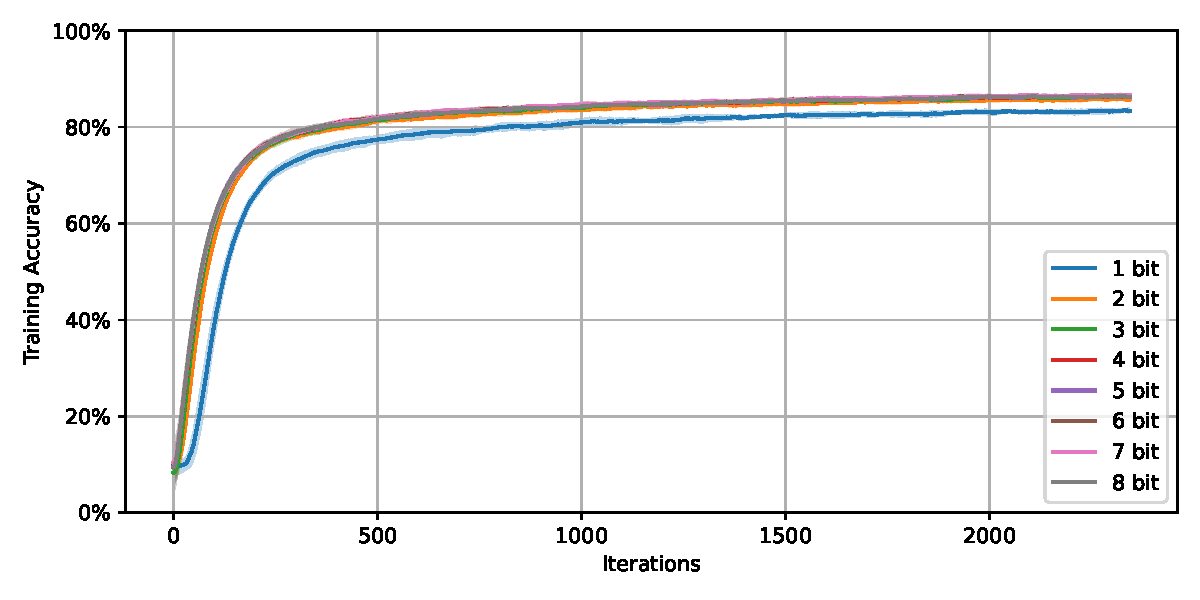
\includegraphics[width=\textwidth]{../standard/FashionMNIST/plots/fashionmnist_train_acc.pdf}
                    \caption{Train Accuracy (smoothed with a window size of 100)}
                \end{subfigure}
                \hfill
                \begin{subfigure}[H]{\textwidth}
                    \centering
                    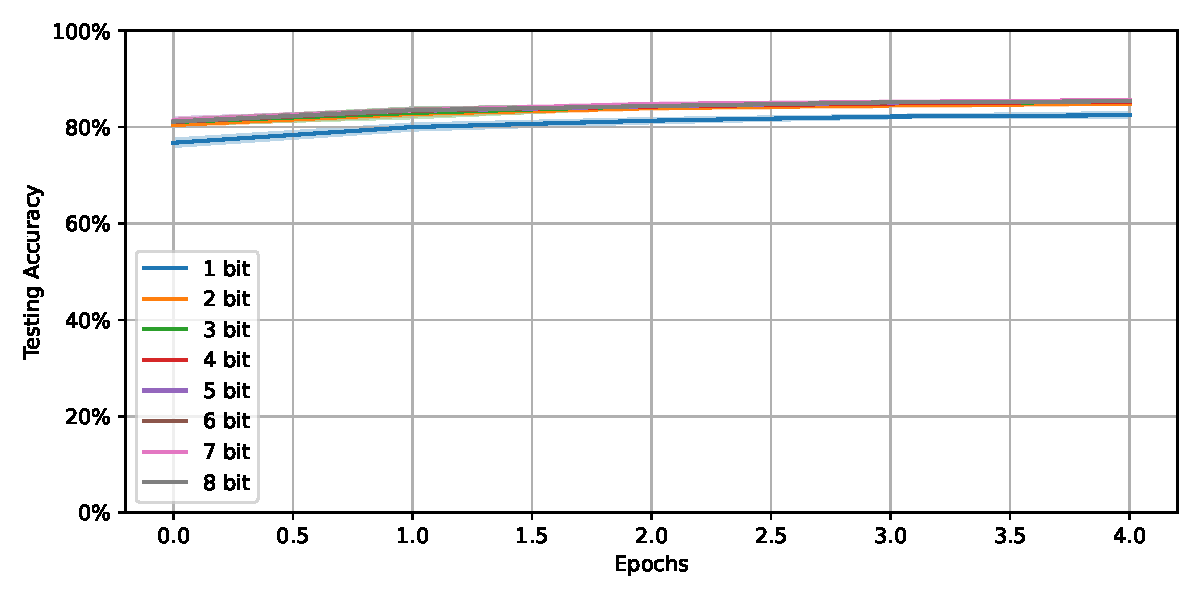
\includegraphics[width=\textwidth]{../standard/FashionMNIST/plots/fashionmnist_test_acc.pdf}
                    \caption{Test Accuracy}
                \end{subfigure}
            \end{subfigure}
            \hfill
            \begin{subfigure}[H]{0.3\textwidth}
                \centering
                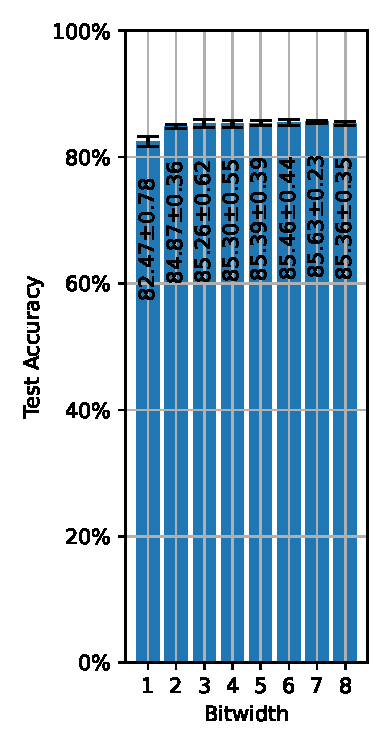
\includegraphics[width=\textwidth]{../standard/FashionMNIST/plots/fashionmnist_final_acc.pdf}
                \caption{Final Test Accuracy}
            \end{subfigure}
            \caption{Accuracy Curves of the Fashion MNIST Model}
        \end{figure}

    \subsection{MNIST}
    \label{appendix:accuracy_curves_mnist}
        Launch command: 
        \begin{lstlisting}[language=Bash, basicstyle=\small, breaklines=true]
python -m test --N 8 --R 10 --T 10 --acc 0.80 --model MNISTNet --data-path /scratch/zyi/codeSpace/data --dataset MNIST --batch-size 128 --opt adam --lr 2e-3 --lr-scheduler none --epochs 5 --lr-warmup-epochs 0 --output-dir /scratch/zyi/codeSpace/MultibitSpikes --mixup-alpha 0.0 --cutmix-alpha 0.0 --label-smoothing 0.0 --disable-amp
        \end{lstlisting}

        \begin{figure}[H]
            \centering
            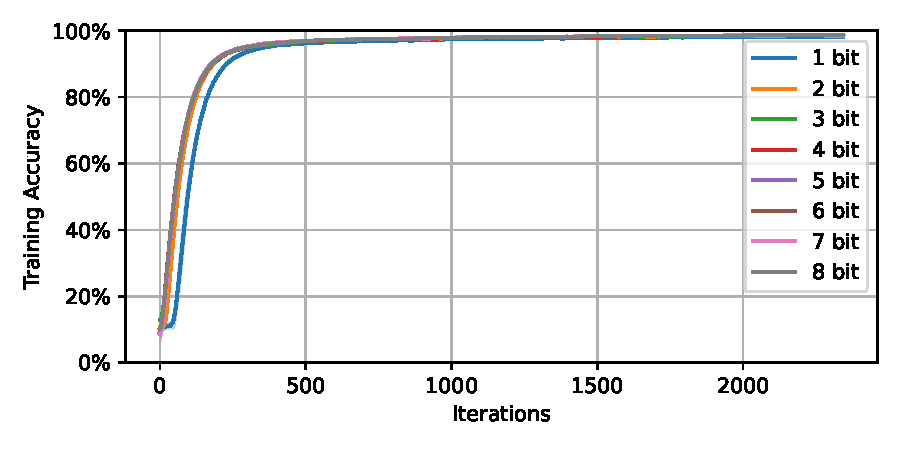
\includegraphics[width=\textwidth]{../standard/MNIST/plots/mnist_train_acc.pdf}
            \caption{Training Accuracy (smoothed with a window size of 100)}
        \end{figure}
        \begin{figure}[H]
            \centering
            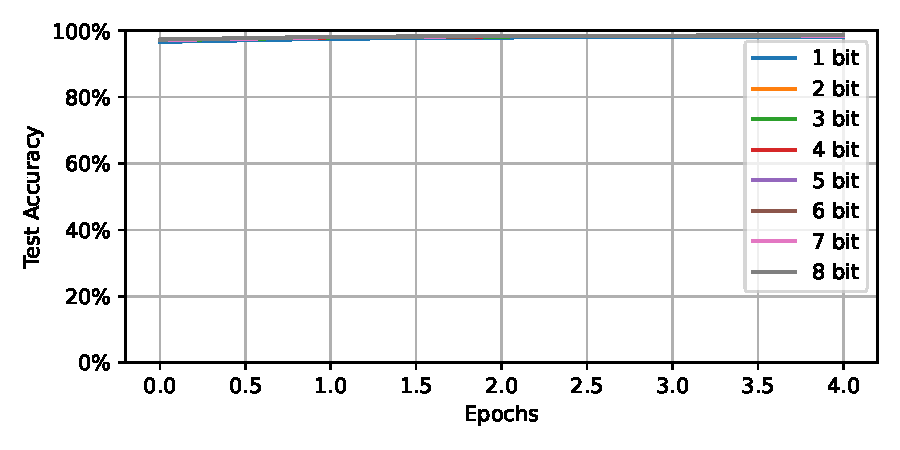
\includegraphics[width=\textwidth]{../standard/MNIST/plots/mnist_test_acc.pdf}
            \caption{Test Accuracy}
        \end{figure}
        \begin{figure}[H]
            \centering
            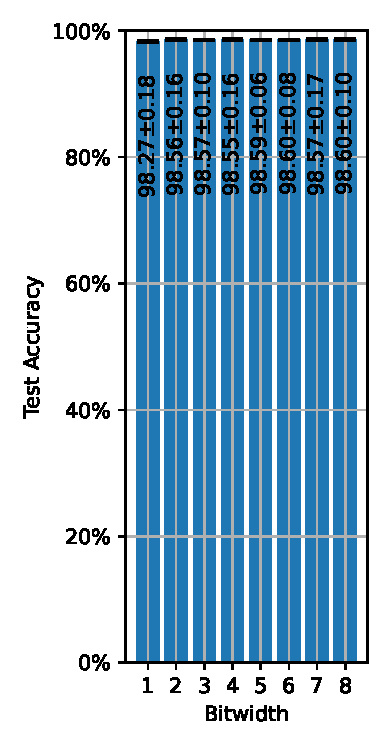
\includegraphics[width=\textwidth]{../standard/MNIST/plots/mnist_final_acc.pdf}
            \caption{Final Test Accuracy}
        \end{figure}
    
    \subsection{NMNIST}
    \label{appendix:accuracy_curves_nmnist}
        Launch command: 
        \begin{lstlisting}[language=Bash, basicstyle=\small, breaklines=true]
python -m test --N 8 --R 10 --T 10 --acc 0.80 --model NMNISTNet --data-path /scratch/zyi/codeSpace/data --dataset NMNIST --batch-size 128 --opt adam --lr 2e-3 --lr-scheduler none --epochs 5 --lr-warmup-epochs 0 --output-dir /scratch/zyi/codeSpace/MultibitSpikes --mixup-alpha 0.0 --cutmix-alpha 0.0 --label-smoothing 0.0 --disable-amp
        \end{lstlisting}

        \begin{figure}[H]
            \centering
            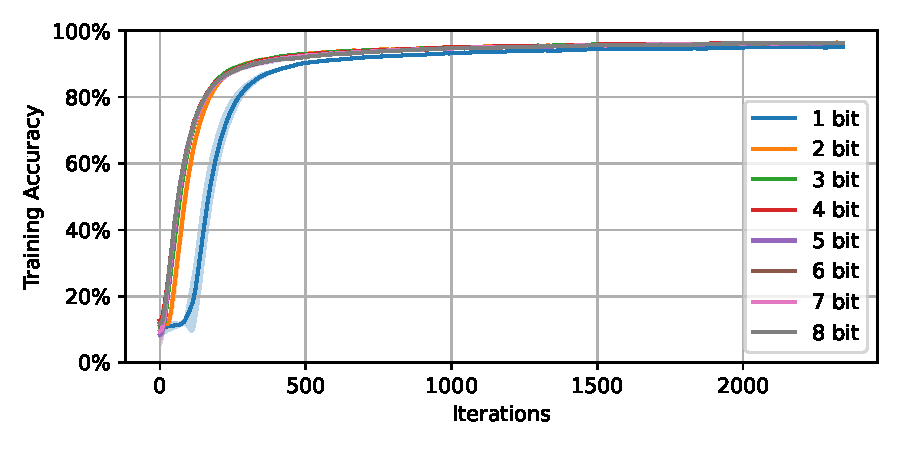
\includegraphics[width=\textwidth]{../standard/NMNIST/plots/nmnist_train_acc.pdf}
            \caption{Training Accuracy (smoothed with a window size of 100)}            
        \end{figure}
        \begin{figure}[H]
            \centering
            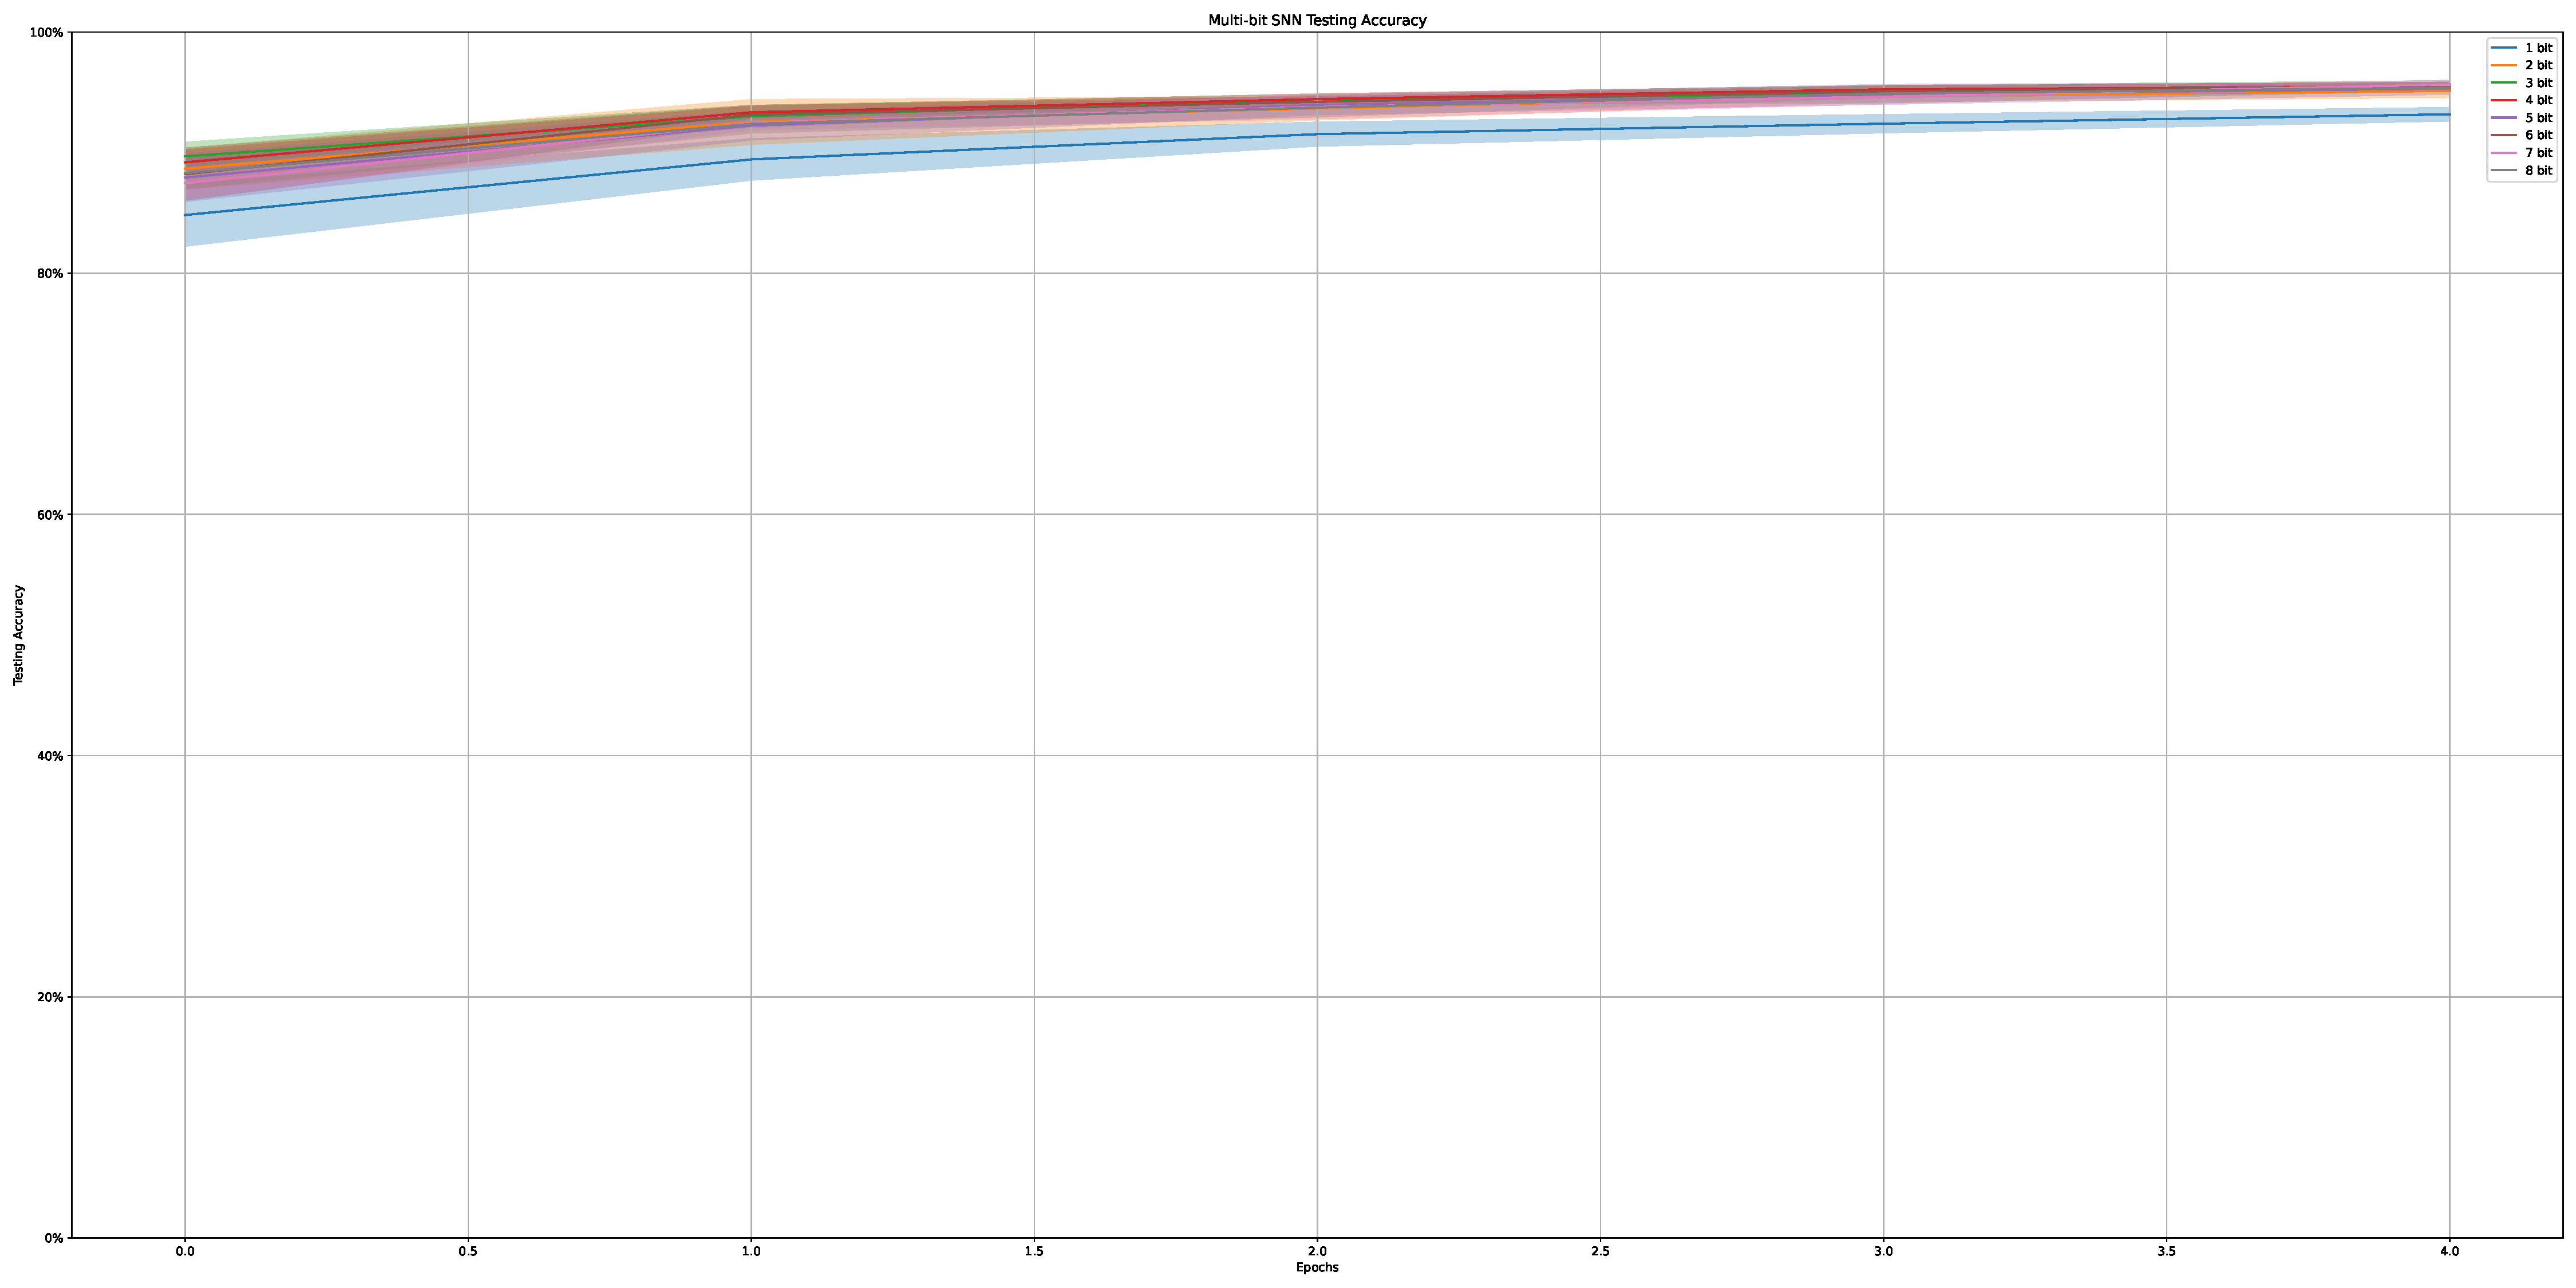
\includegraphics[width=\textwidth]{../standard/NMNIST/plots/nmnist_test_acc.pdf}
            \caption{Test Accuracy}
        \end{figure}
        \begin{figure}[H]
            \centering
            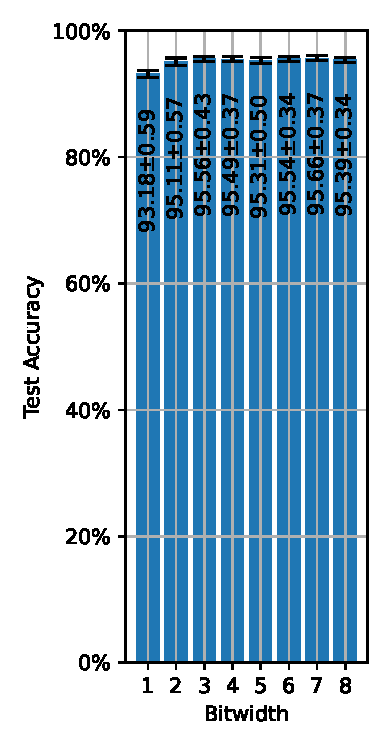
\includegraphics[width=\textwidth]{../standard/NMNIST/plots/nmnist_final_acc.pdf}
            \caption{Final Test Accuracy}
        \end{figure}

    \subsection{DVS Gesture}
    \label{appendix:accuracy_curves_dvs_gesture}
        Launch command: 
        \begin{lstlisting}[language=Bash, basicstyle=\small, breaklines=true]
python -m test --N 8 --R 10 --T 10 --acc 0.80 --model DVSGestureNet --data-path /scratch/zyi/codeSpace/data --dataset DVSGesture --batch-size 128 --opt adam --lr 1e-3 --lr-scheduler cosa --epochs 20 --lr-warmup-epochs 0 --output-dir /scratch/zyi/codeSpace/MultibitSpikes
        \end{lstlisting}

        \begin{figure}[H]
            \centering
            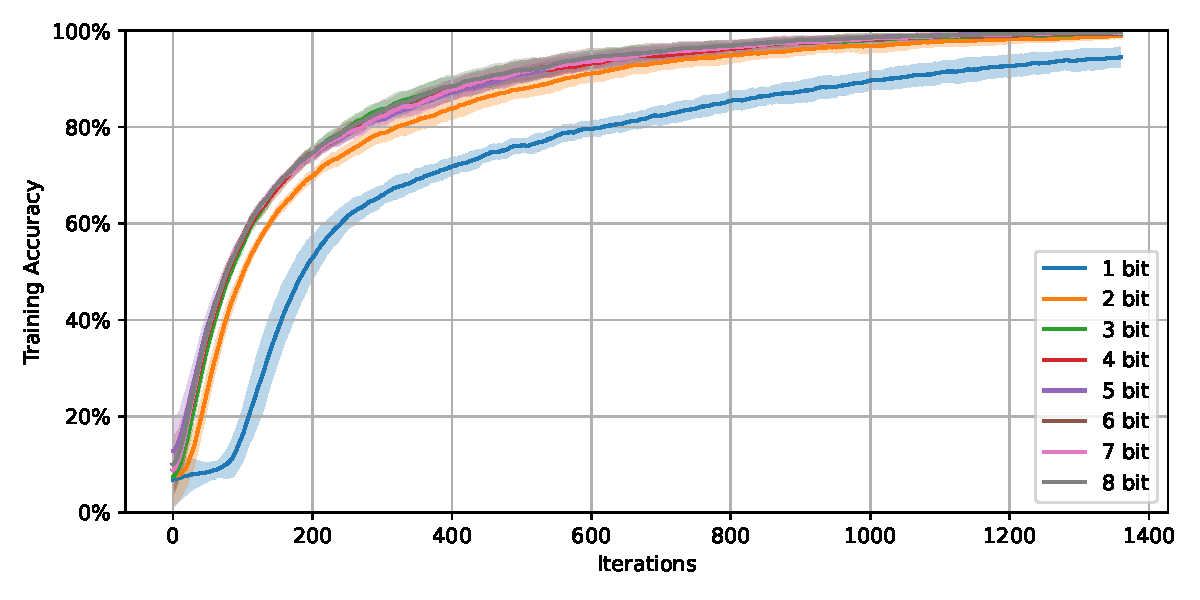
\includegraphics[width=\textwidth]{../standard/DVSGesture/plots/dvsgesture_train_acc.pdf}
            \caption{Training Accuracy (smoothed with a window size of 100)}
        \end{figure}
        \begin{figure}[H]
            \centering
            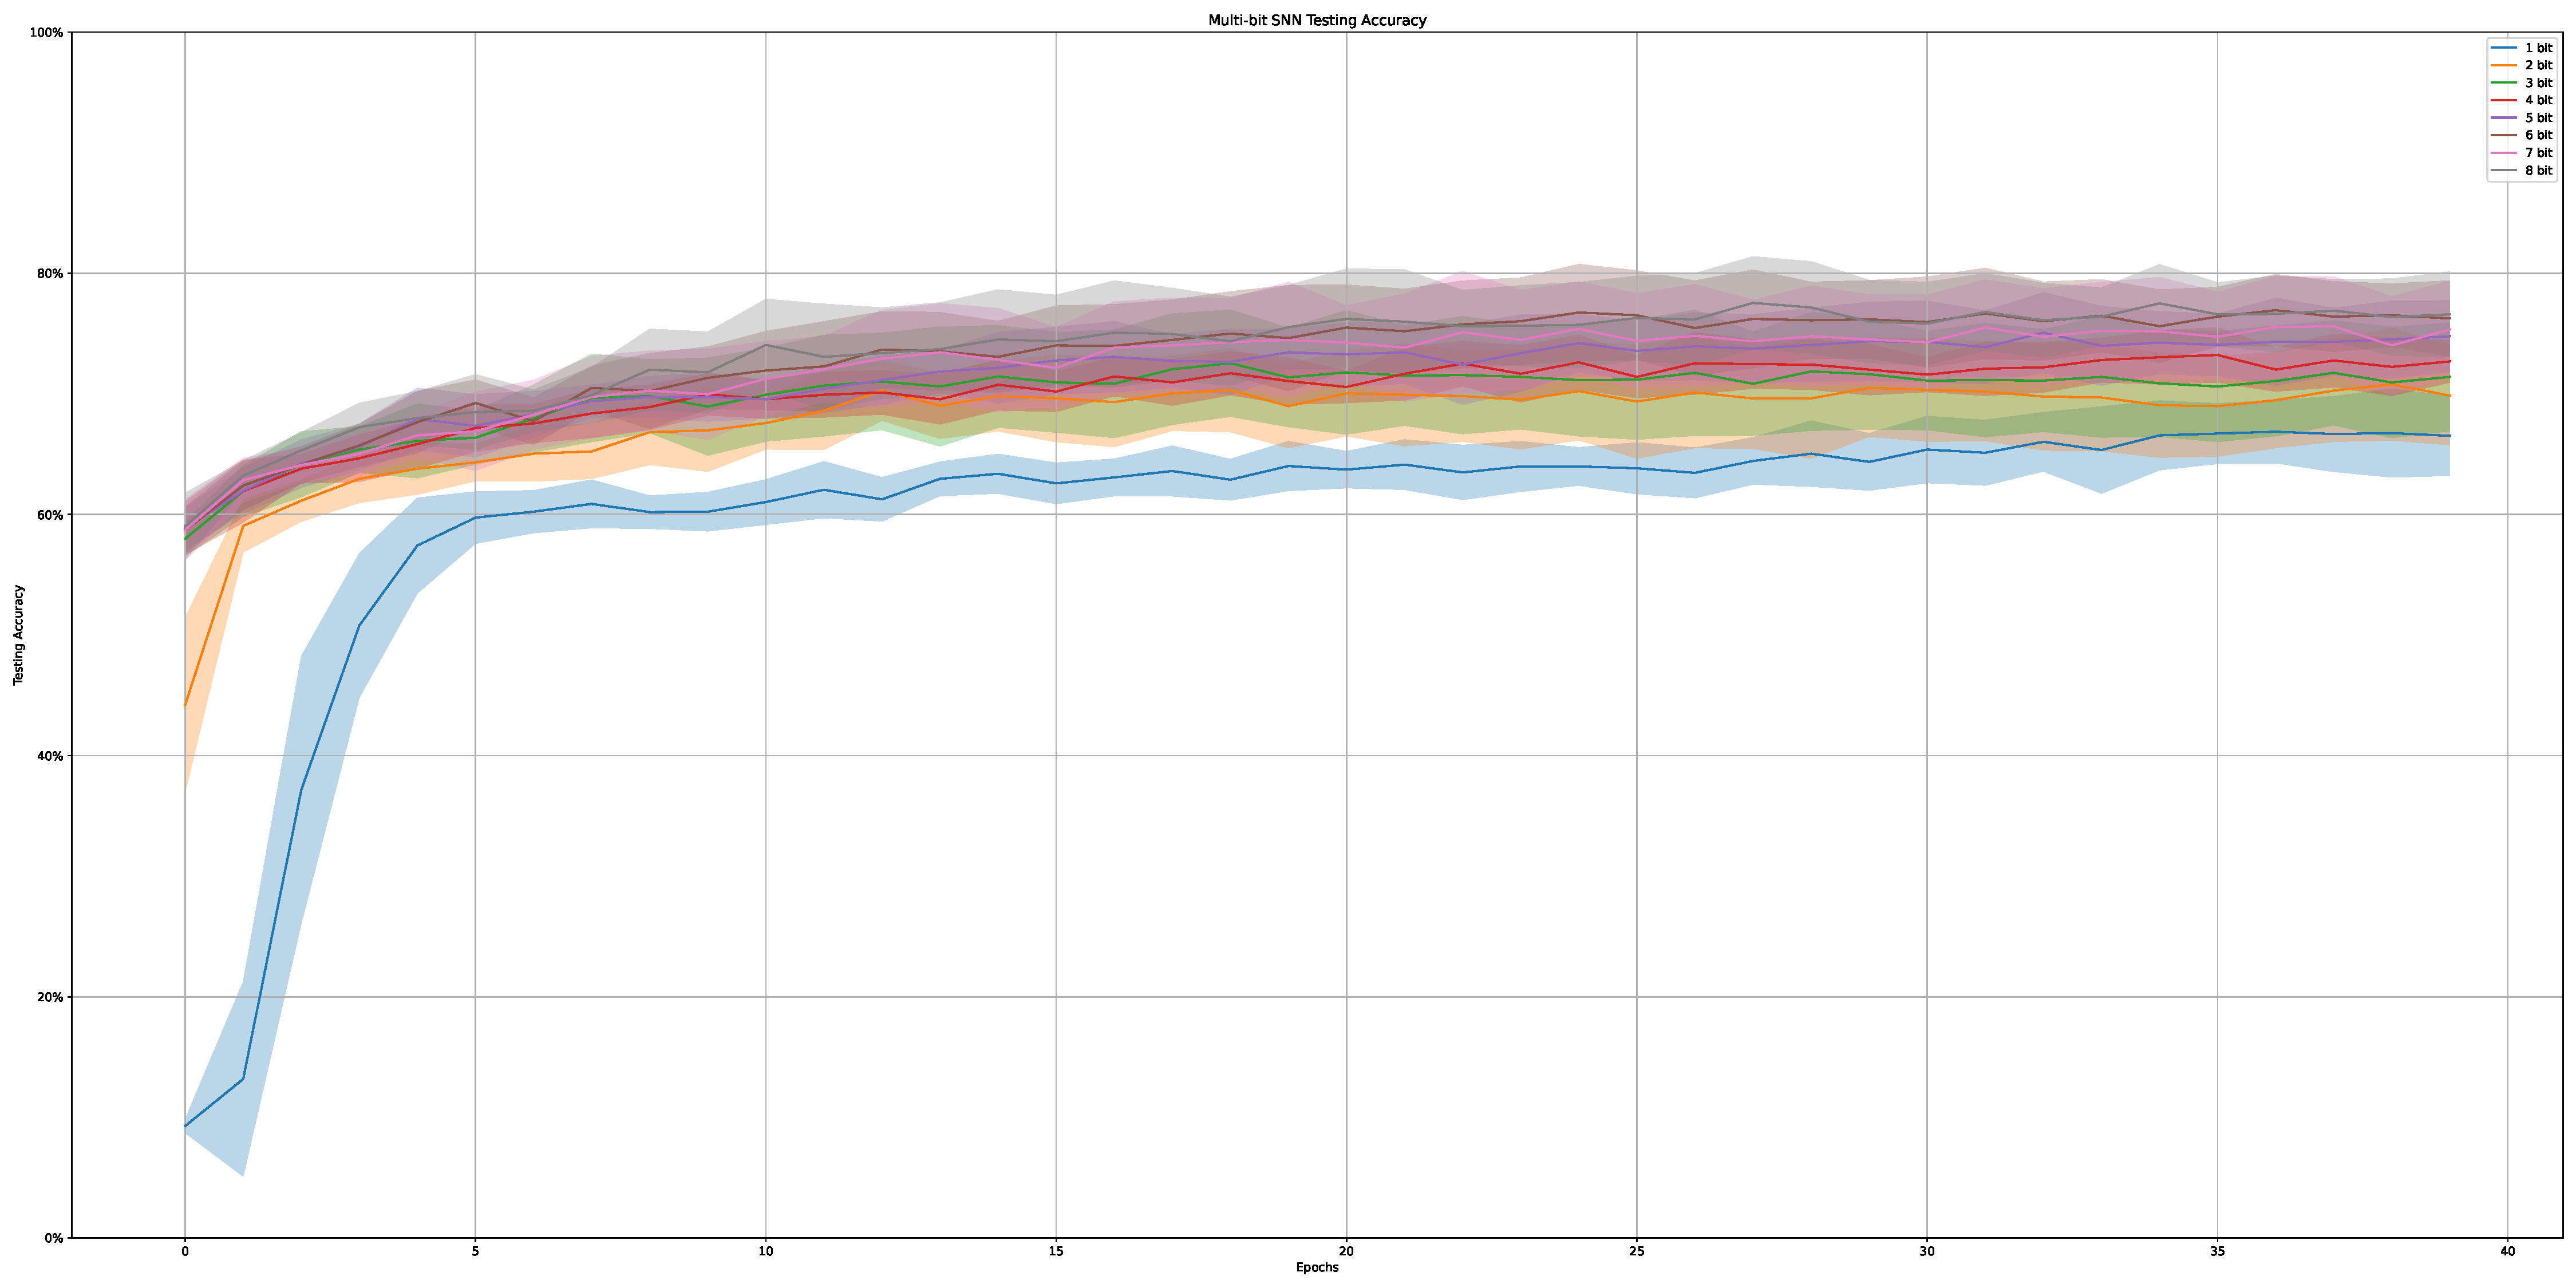
\includegraphics[width=\textwidth]{../standard/DVSGesture/plots/dvsgesture_test_acc.pdf}
            \caption{Test Accuracy}
        \end{figure}
        \begin{figure}[H]
            \centering
            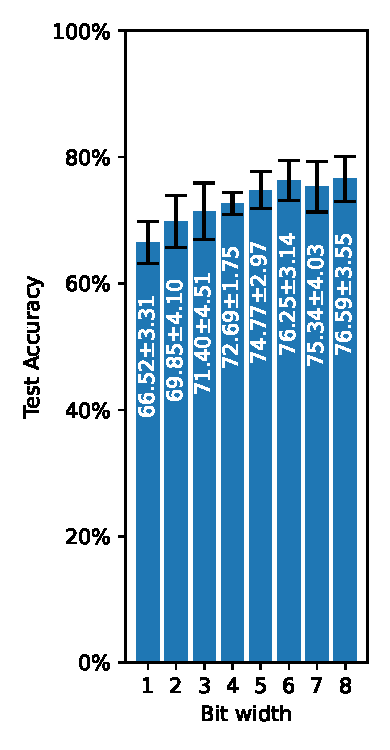
\includegraphics[width=\textwidth]{../standard/DVSGesture/plots/dvsgesture_final_acc.pdf}
            \caption{Final Test Accuracy}
        \end{figure}

    \subsection{CIFAR-10}
    \label{appendix:accuracy_curves_cifar10}
        Launch command: 
        \begin{lstlisting}[language=Bash, basicstyle=\small, breaklines=true]
python -m test --N 4 --R 5 --T 10 --acc 0.80 --model CIFAR10Net --data-path /scratch/zyi/codeSpace/data --dataset CIFAR10 --batch-size 128 --opt adam --lr 1e-5 --lr-scheduler none --epochs 50 --lr-warmup-epochs 0 --output-dir /scratch/zyi/codeSpace/MultibitSpikes
        \end{lstlisting}

        \begin{figure}[H]
            \centering
            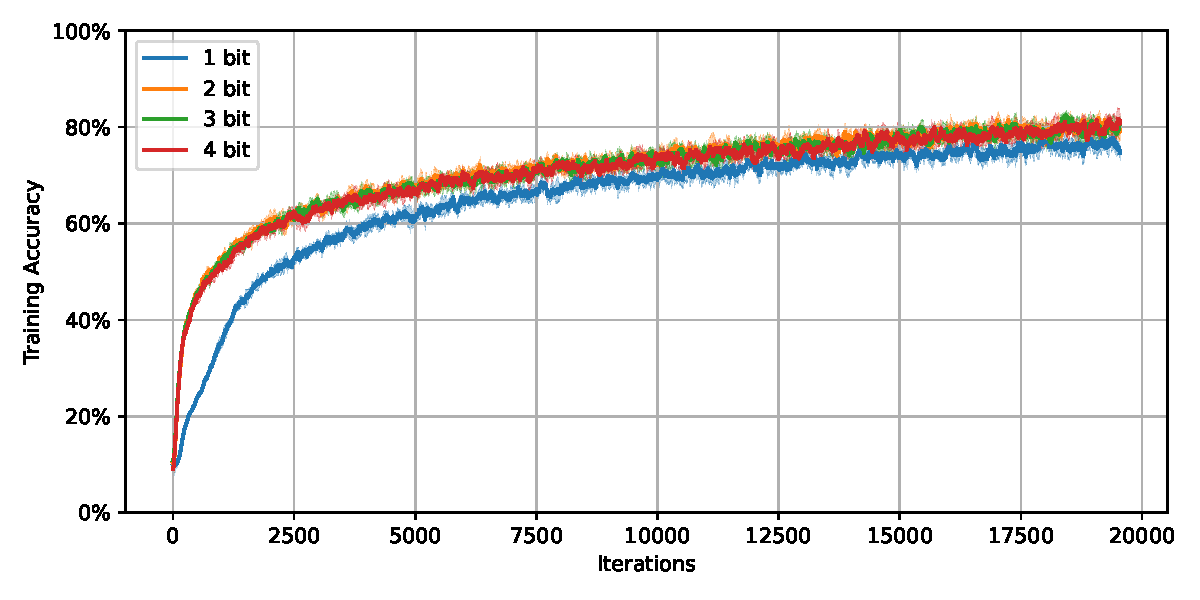
\includegraphics[width=\textwidth]{../standard/CIFAR10/plots/cifar10_train_acc.pdf}
            \caption{Training Accuracy (smoothed with a window size of 100)}
        \end{figure}
        \begin{figure}[H]
            \centering
            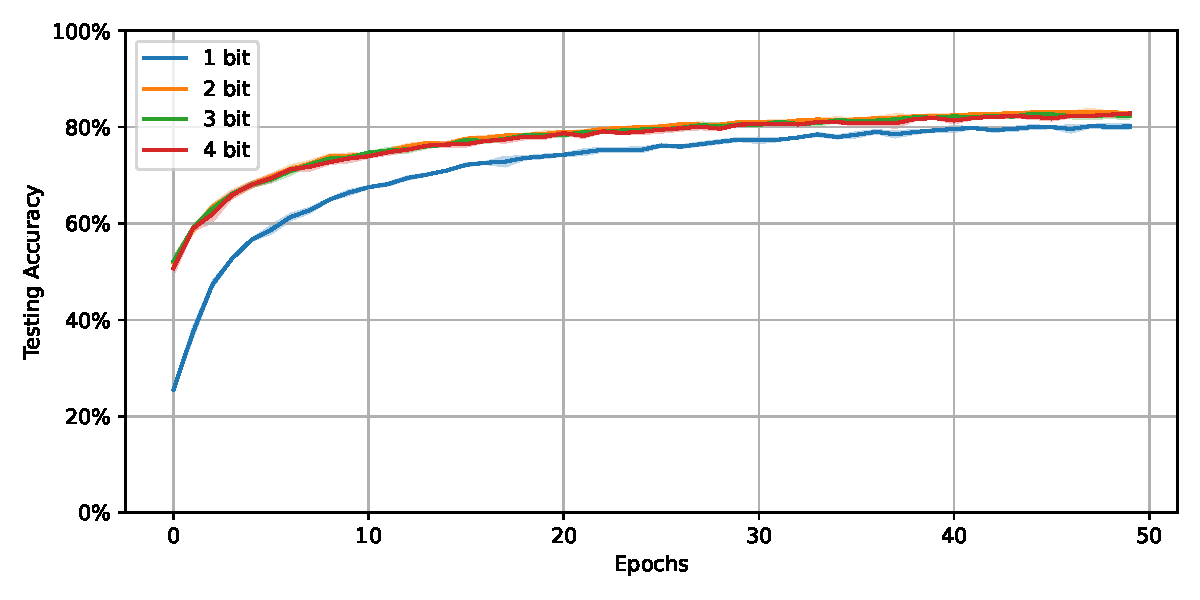
\includegraphics[width=\textwidth]{../standard/CIFAR10/plots/cifar10_test_acc.pdf}
            \caption{Test Accuracy}
        \end{figure}
        \begin{figure}[H]
            \centering
            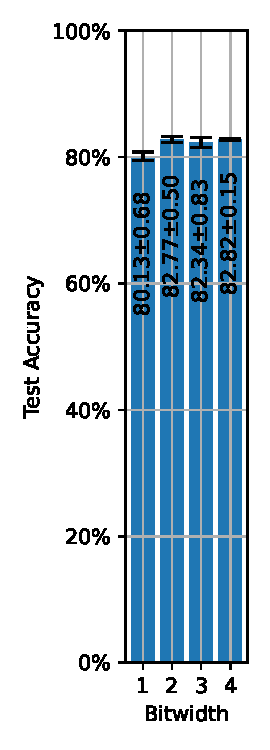
\includegraphics[width=\textwidth]{../standard/CIFAR10/plots/cifar10_final_acc.pdf}
            \caption{Final Test Accuracy}
        \end{figure}

\section{Iterations to Reach the Target Accuracy of 80\%}
\label{appendix:iterations}

    \subsection{Fashion MNIST}
    \label{appendix:iterations_fashion_mnist}
        Launch command: Same as in Appendix \ref{appendix:accuracy_curves_fashion_mnist}
        \begin{figure}[H]
            \centering
            \begin{subfigure}[H]{0.495\textwidth}
                \centering
                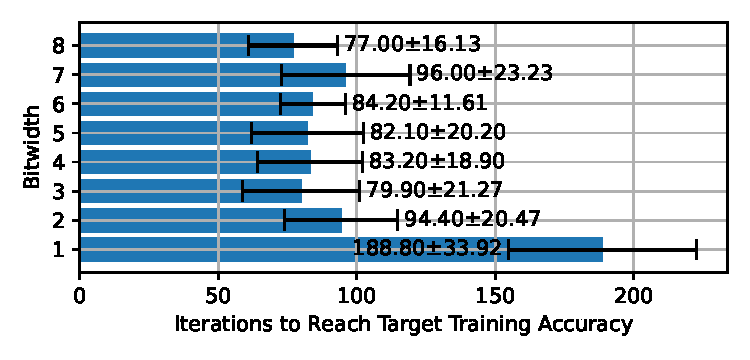
\includegraphics[width=\textwidth]{../standard/FashionMNIST/plots/fashionmnist_train_iters_horizontal.pdf}
                \caption{Iterations to Reach the Training Accuracy}
            \end{subfigure}
            \hfill
            \begin{subfigure}[H]{0.495\textwidth}
                \centering
                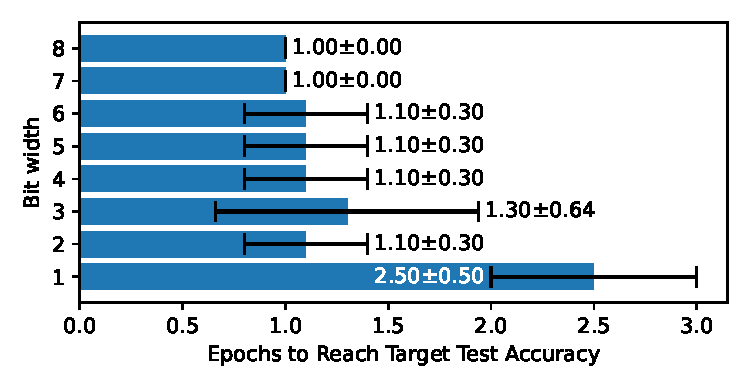
\includegraphics[width=\textwidth]{../standard/FashionMNIST/plots/fashionmnist_test_iters_horizontal.pdf}
                \caption{Iterations to Reach the Test Accuracy}
            \end{subfigure}
            \caption{Iterations to Reach the Target Accuracy of 80\%}
        \end{figure}

    \subsection{MNIST}
    \label{appendix:iterations_mnist}
        Launch command: Same as in Appendix \ref{appendix:accuracy_curves_mnist}
        \begin{figure}[H]
            \centering
            \begin{subfigure}[H]{0.48\textwidth}
                \centering
                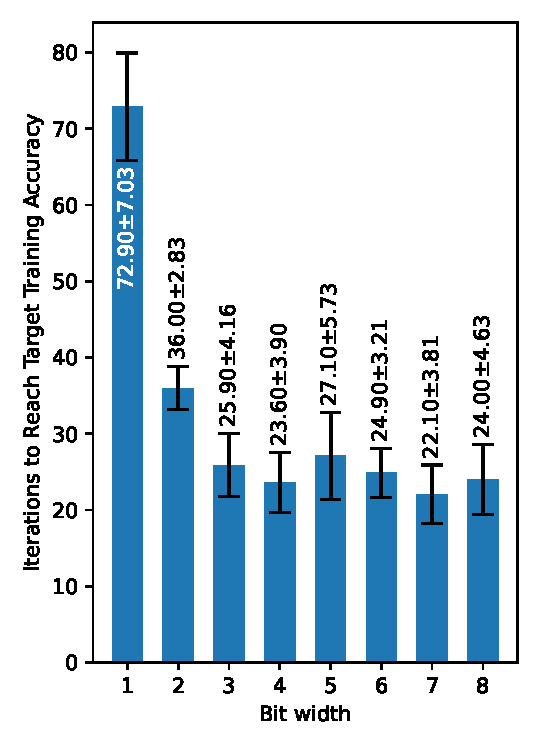
\includegraphics[width=\textwidth]{../standard/MNIST/plots/mnist_train_iters.pdf}
                \caption{Iterations to Reach the Training Accuracy}
            \end{subfigure}
            \hfill
            \begin{subfigure}[H]{0.48\textwidth}
                \centering
                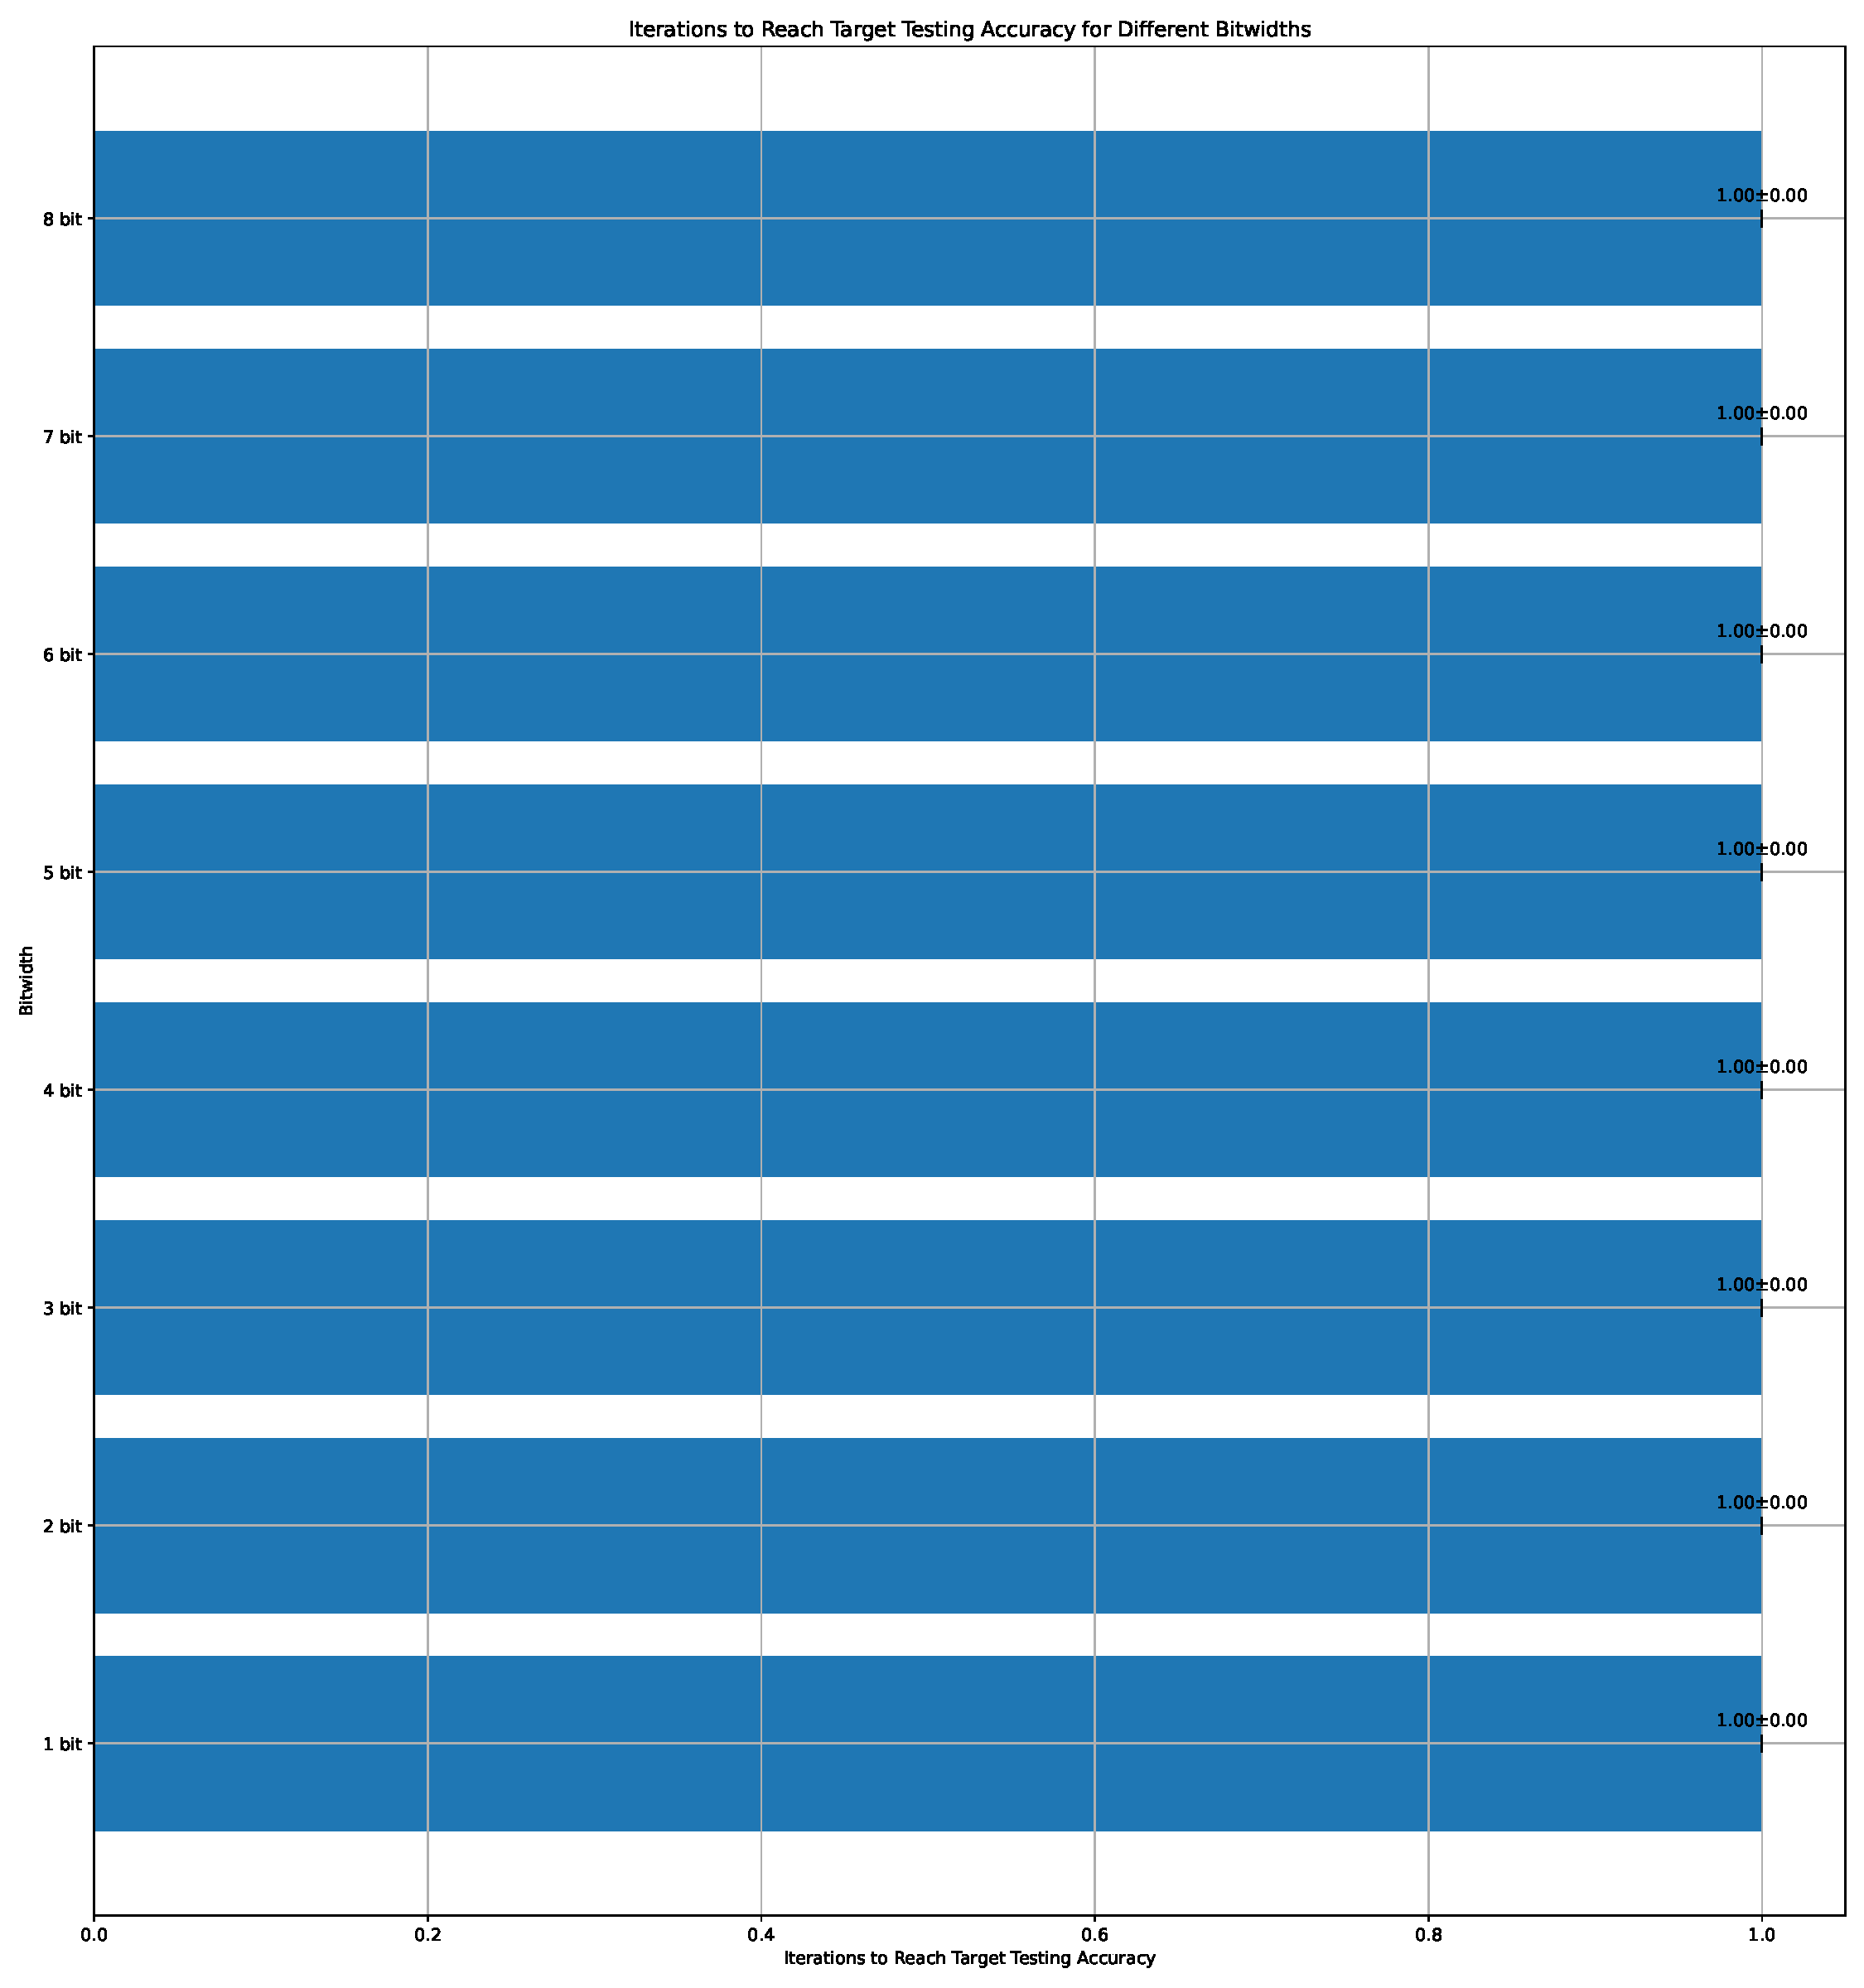
\includegraphics[width=\textwidth]{../standard/MNIST/plots/mnist_test_iters.pdf}
                \caption{Iterations to Reach the Test Accuracy}
            \end{subfigure}
            \caption{Iterations to Reach the Target Accuracy of 80\%}
        \end{figure}

    \subsection{NMNIST}
    \label{appendix:iterations_nmnist}
        Launch command: Same as in Appendix \ref{appendix:accuracy_curves_nmnist}
        \begin{figure}[H]
            \centering
            \begin{subfigure}[H]{0.48\textwidth}
                \centering
                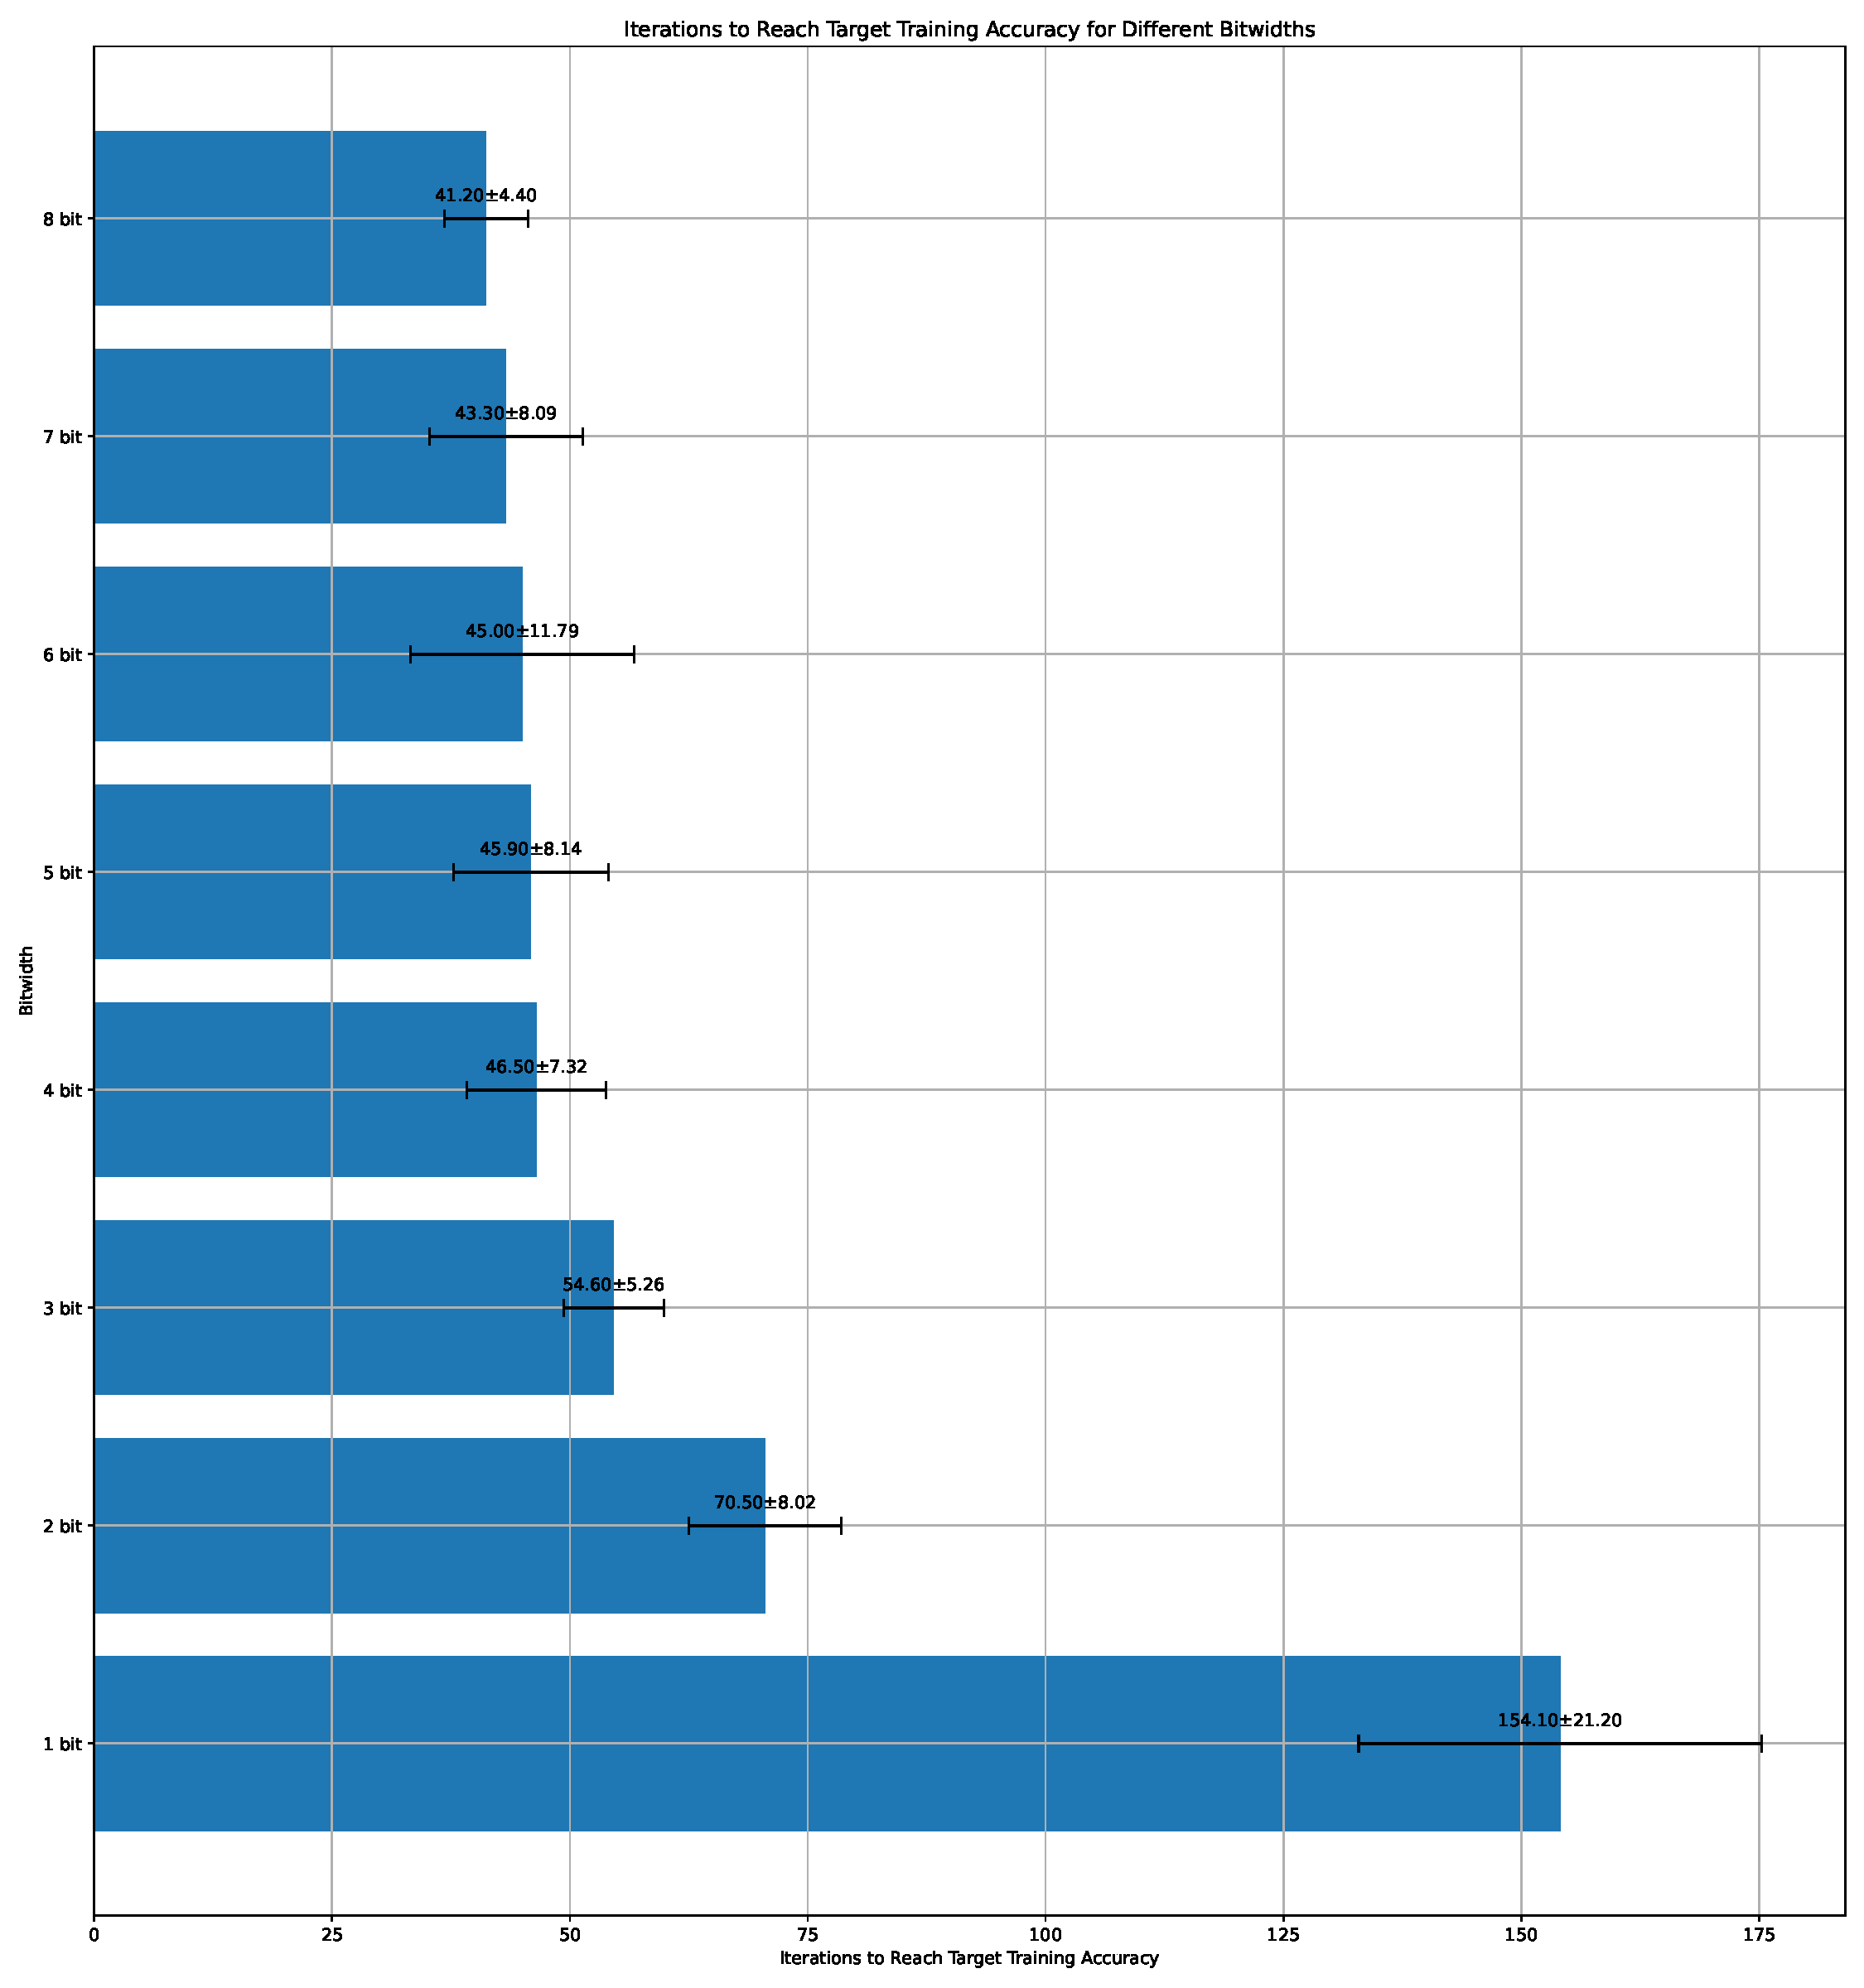
\includegraphics[width=\textwidth]{../standard/NMNIST/plots/nmnist_train_iters.pdf}
                \caption{Iterations to Reach the Training Accuracy}
            \end{subfigure}
            \hfill
            \begin{subfigure}[H]{0.48\textwidth}
                \centering
                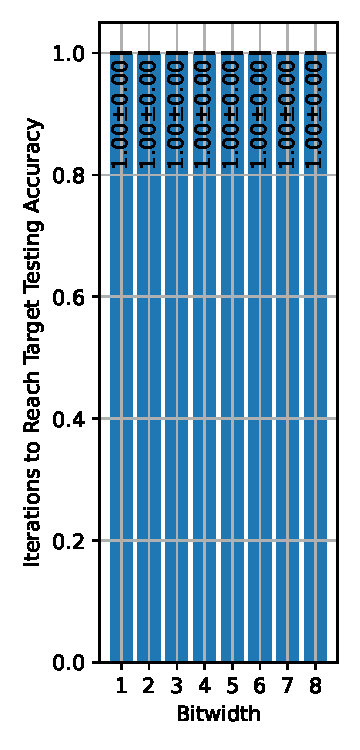
\includegraphics[width=\textwidth]{../standard/NMNIST/plots/nmnist_test_iters.pdf}
                \caption{Iterations to Reach the Test Accuracy}
            \end{subfigure}
            \caption{Iterations to Reach the Target Accuracy of 80\%}
        \end{figure}

    \subsection{DVS Gesture}
    \label{appendix:iterations_dvs_gesture}
        Launch command: Same as in Appendix \ref{appendix:accuracy_curves_dvs_gesture}
        \begin{figure}[H]
            \centering
            \begin{subfigure}[H]{0.48\textwidth}
                \centering
                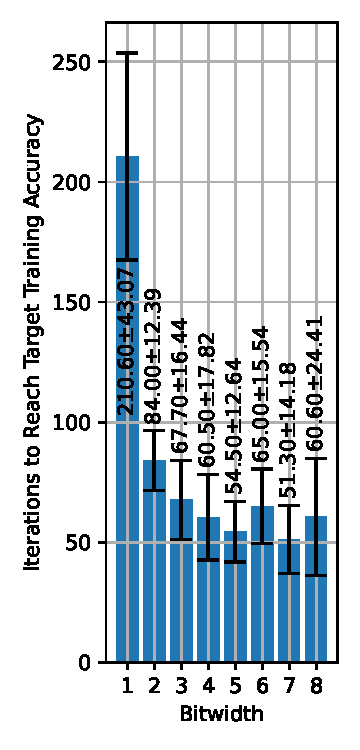
\includegraphics[width=\textwidth]{../standard/DVSGesture/plots/dvsgesture_train_iters.pdf}
                \caption{Iterations to Reach the Training Accuracy}
            \end{subfigure}
            \hfill
            \begin{subfigure}[H]{0.48\textwidth}
                \centering
                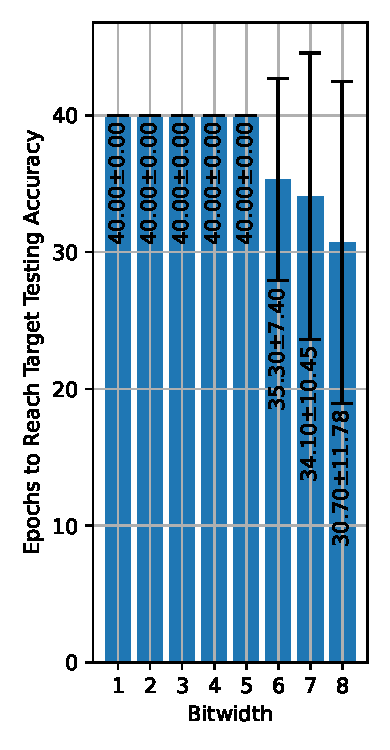
\includegraphics[width=\textwidth]{../standard/DVSGesture/plots/dvsgesture_test_iters.pdf}
                \caption{Iterations to Reach the Test Accuracy}
            \end{subfigure}
            \caption{Iterations to Reach the Target Accuracy of 80\%}
        \end{figure}

    Notice that we encountered overfitting in the DVS Gesture dataset, which is why the number of iterations to reach the target test accuracy is capped at 40 epochs (the maximum number of epochs in the training process), thus not representative. 

    \subsection{CIFAR-10}
    \label{appendix:iterations_cifar10}
        Launch command: Same as in Appendix \ref{appendix:accuracy_curves_cifar10}
        \begin{figure}[H]
            \centering
            \begin{subfigure}[H]{0.48\textwidth}
                \centering
                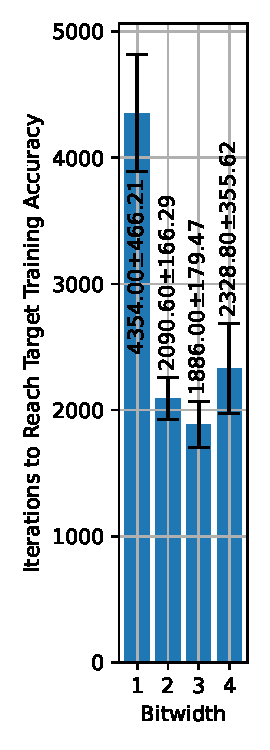
\includegraphics[width=\textwidth]{../standard/CIFAR10/plots/cifar10_train_iters.pdf}
                \caption{Iterations to Reach the Training Accuracy}
            \end{subfigure}
            \hfill
            \begin{subfigure}[H]{0.48\textwidth}
                \centering
                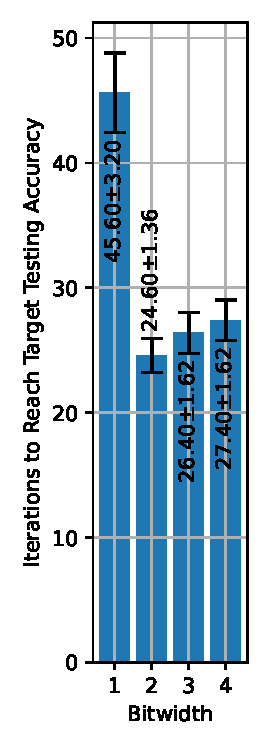
\includegraphics[width=\textwidth]{../standard/CIFAR10/plots/cifar10_test_iters.pdf}
                \caption{Iterations to Reach the Test Accuracy}
            \end{subfigure}
            \caption{Iterations to Reach the Target Accuracy of 80\%}
        \end{figure}



\chapter{Firing Rate in Different Positions of the Multi-Bit Spike Train Model}
\label{appendix:firerate}

    For the ease of debugging, the first measuring position is always just the input data. If the data is captured by a dynamic vision sensor or it is encoded with a Poisson spike generator, one should see a firing rate much below 100\%. In the case of original data (e.g. CIFAR-10), the firing rate should be close to 100\%. 

    From the second measuring position to the last position, the firing rate is measured after the LIF neuron layers. Not all LIF neuron layers are measured. But the last LIF neuron layer is always measured. 

    \section{Fashion MNIST}
    \label{appendix:firerate_fashion_mnist}
        Launch command: 
        \begin{lstlisting}[language=Bash, basicstyle=\small, breaklines=true]
python -m test --N 2 --R 10 --T 10 10 --acc 0.80 --model FashionMNISTNet --data-path /scratch/zyi/codeSpace/data --dataset FashionMNIST --batch-size 128 --opt adam --lr 2e-3 --lr-scheduler none --epochs 50 --lr-warmup-epochs 0 --output-dir /scratch/zyi/codeSpace/MultibitSpikes/firerate --mixup-alpha 0.0 --cutmix-alpha 0.0 --label-smoothing 0.0 --disable-amp
        \end{lstlisting}

        \begin{figure}[H]
            \centering
            \begin{subfigure}[H]{0.48\textwidth}
                \centering
                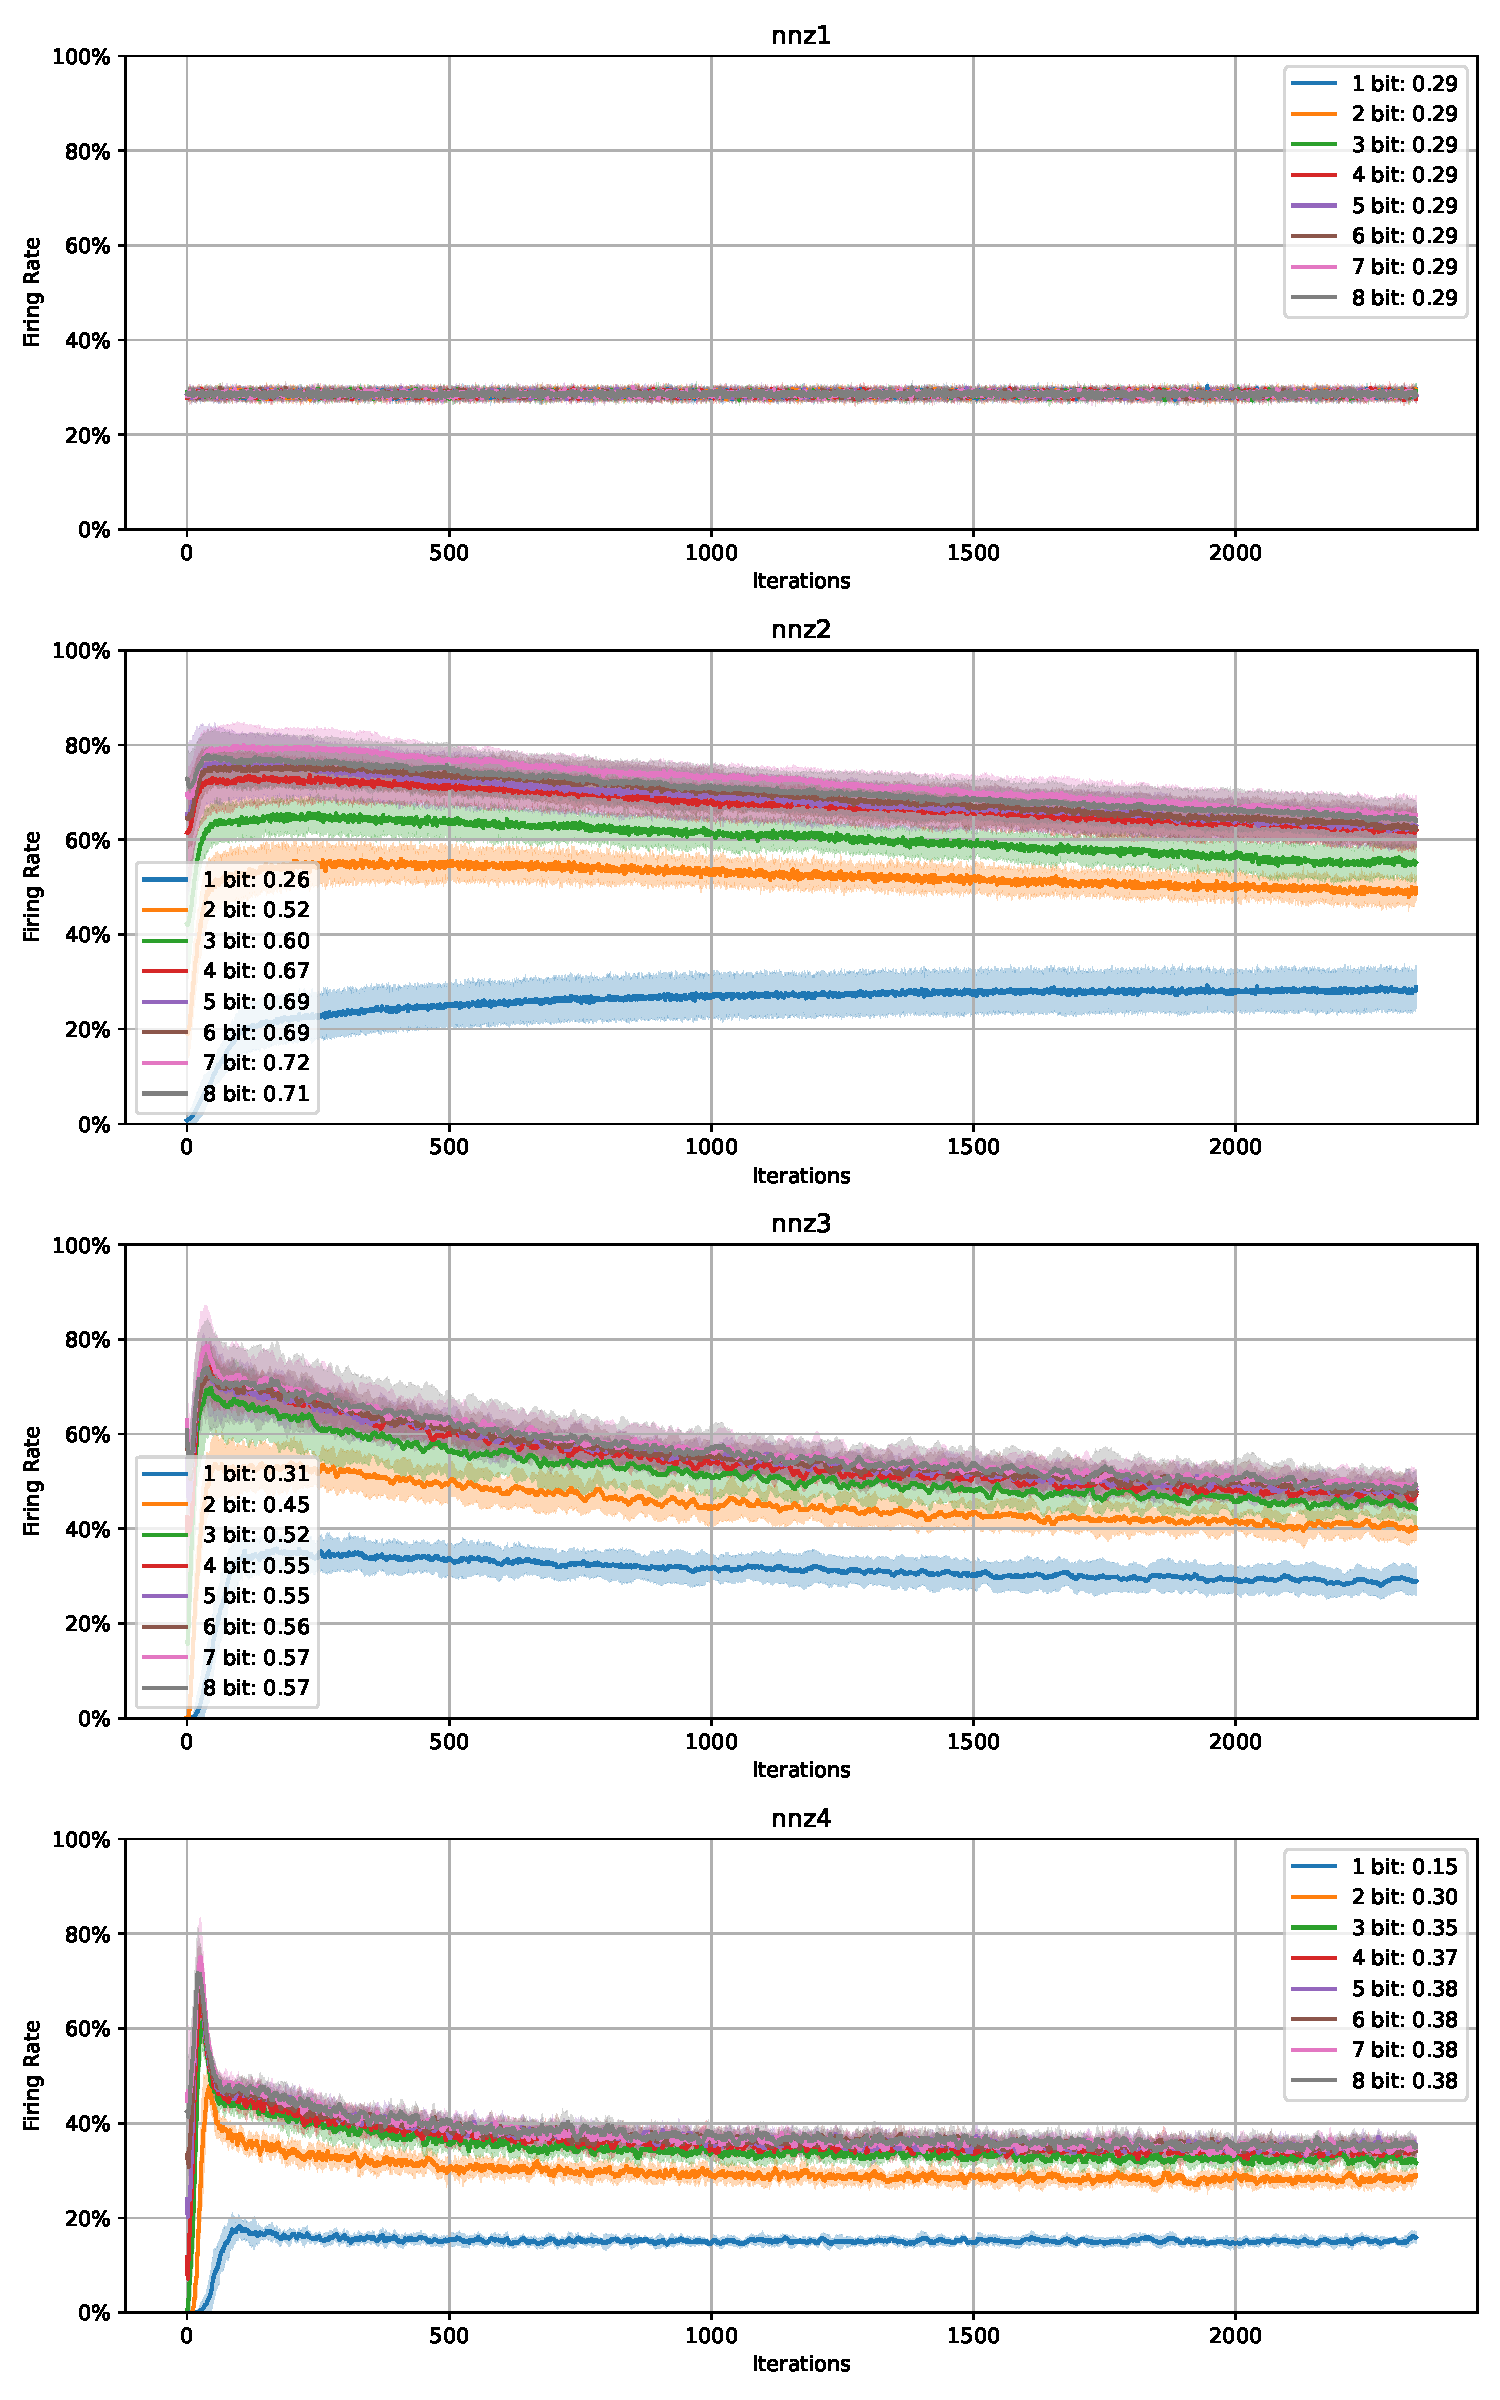
\includegraphics[width=\textwidth]{../firerate/FashionMNIST/plots/fashionmnist_train_firerate.pdf}
                \caption{Firing Rate in Different Positions (Training)}
            \end{subfigure}
            \hfill
            \begin{subfigure}[H]{0.48\textwidth}
                \centering
                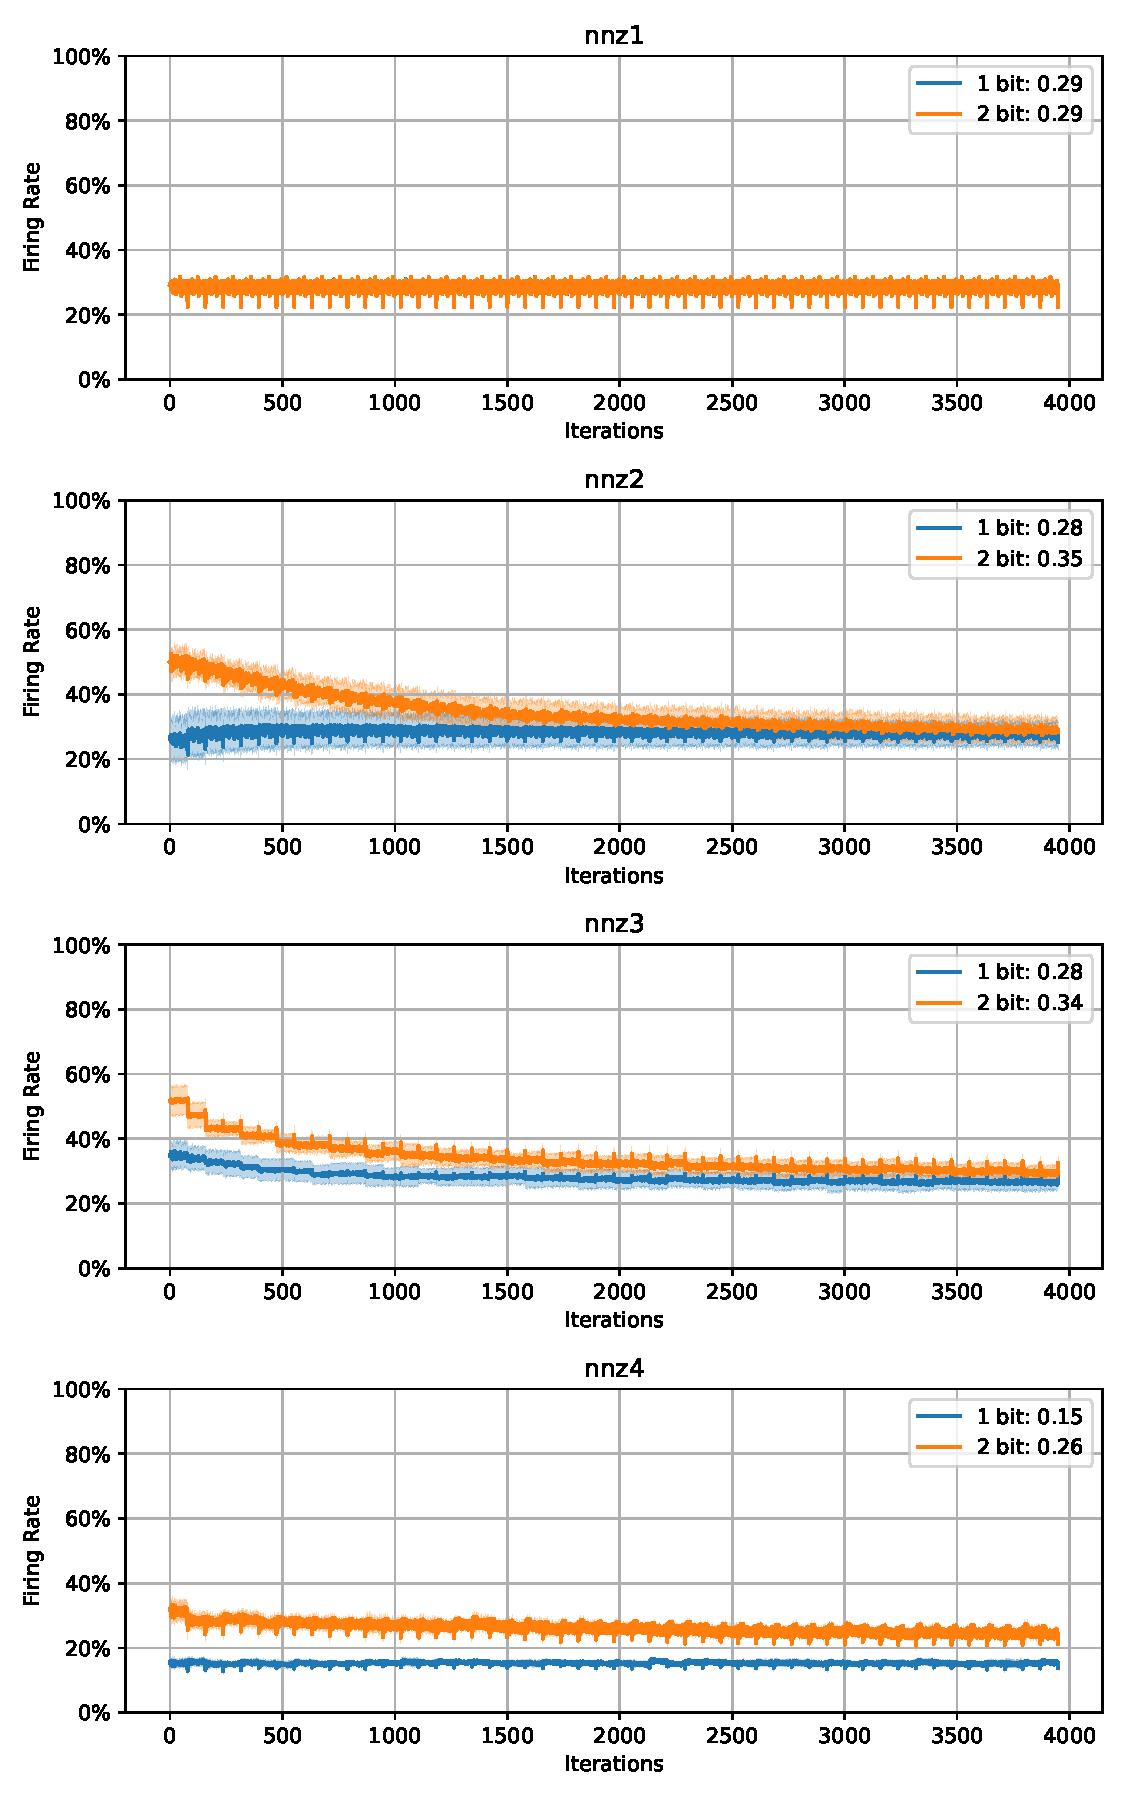
\includegraphics[width=\textwidth]{../firerate/FashionMNIST/plots/fashionmnist_test_firerate.pdf}
                \caption{Firing Rate in Different Positions (Test)}
            \end{subfigure}
            \hfill
            \begin{subfigure}[H]{\textwidth}
                \centering
                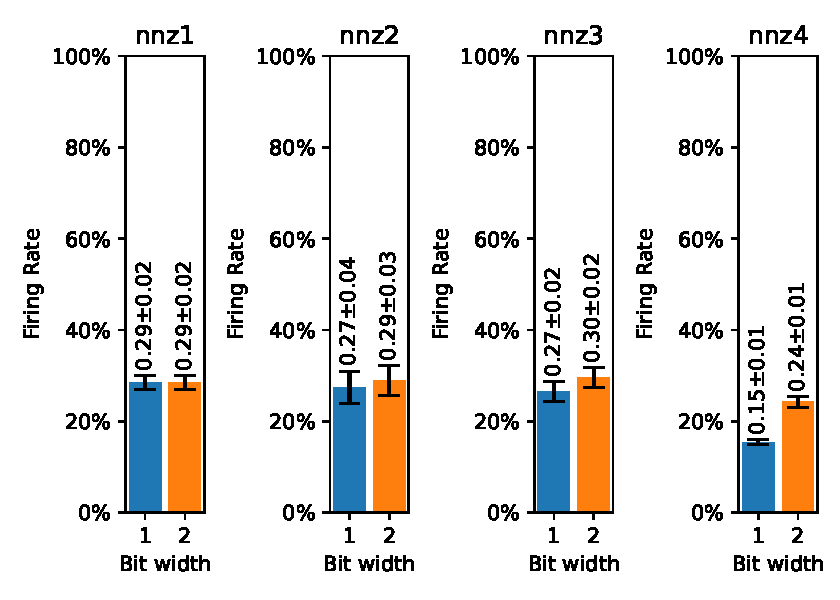
\includegraphics[width=\textwidth]{../firerate/FashionMNIST/plots/fashionmnist_final_firerate.pdf}
                \caption{Firing Rate in Different Positions (Final Test)}
            \end{subfigure}
            \caption{Firing Rate in Different Positions of the Fashion MNIST Model}
        \end{figure}

    \section{MNIST}
    \label{appendix:firerate_mnist}
        Launch command: 
        \begin{lstlisting}[language=Bash, basicstyle=\small, breaklines=true]
python -m test --N 2 --R 10 --T 10 10 --acc 0.80 --model MNISTNet --data-path /scratch/zyi/codeSpace/data --dataset MNIST --batch-size 128 --opt adam --lr 2e-3 --lr-scheduler none --epochs 50 --lr-warmup-epochs 0 --output-dir /scratch/zyi/codeSpace/MultibitSpikes/firerate --mixup-alpha 0.0 --cutmix-alpha 0.0 --label-smoothing 0.0 --disable-amp
        \end{lstlisting}

        \begin{figure}[H]
            \centering
            \begin{subfigure}[H]{0.48\textwidth}
                \centering
                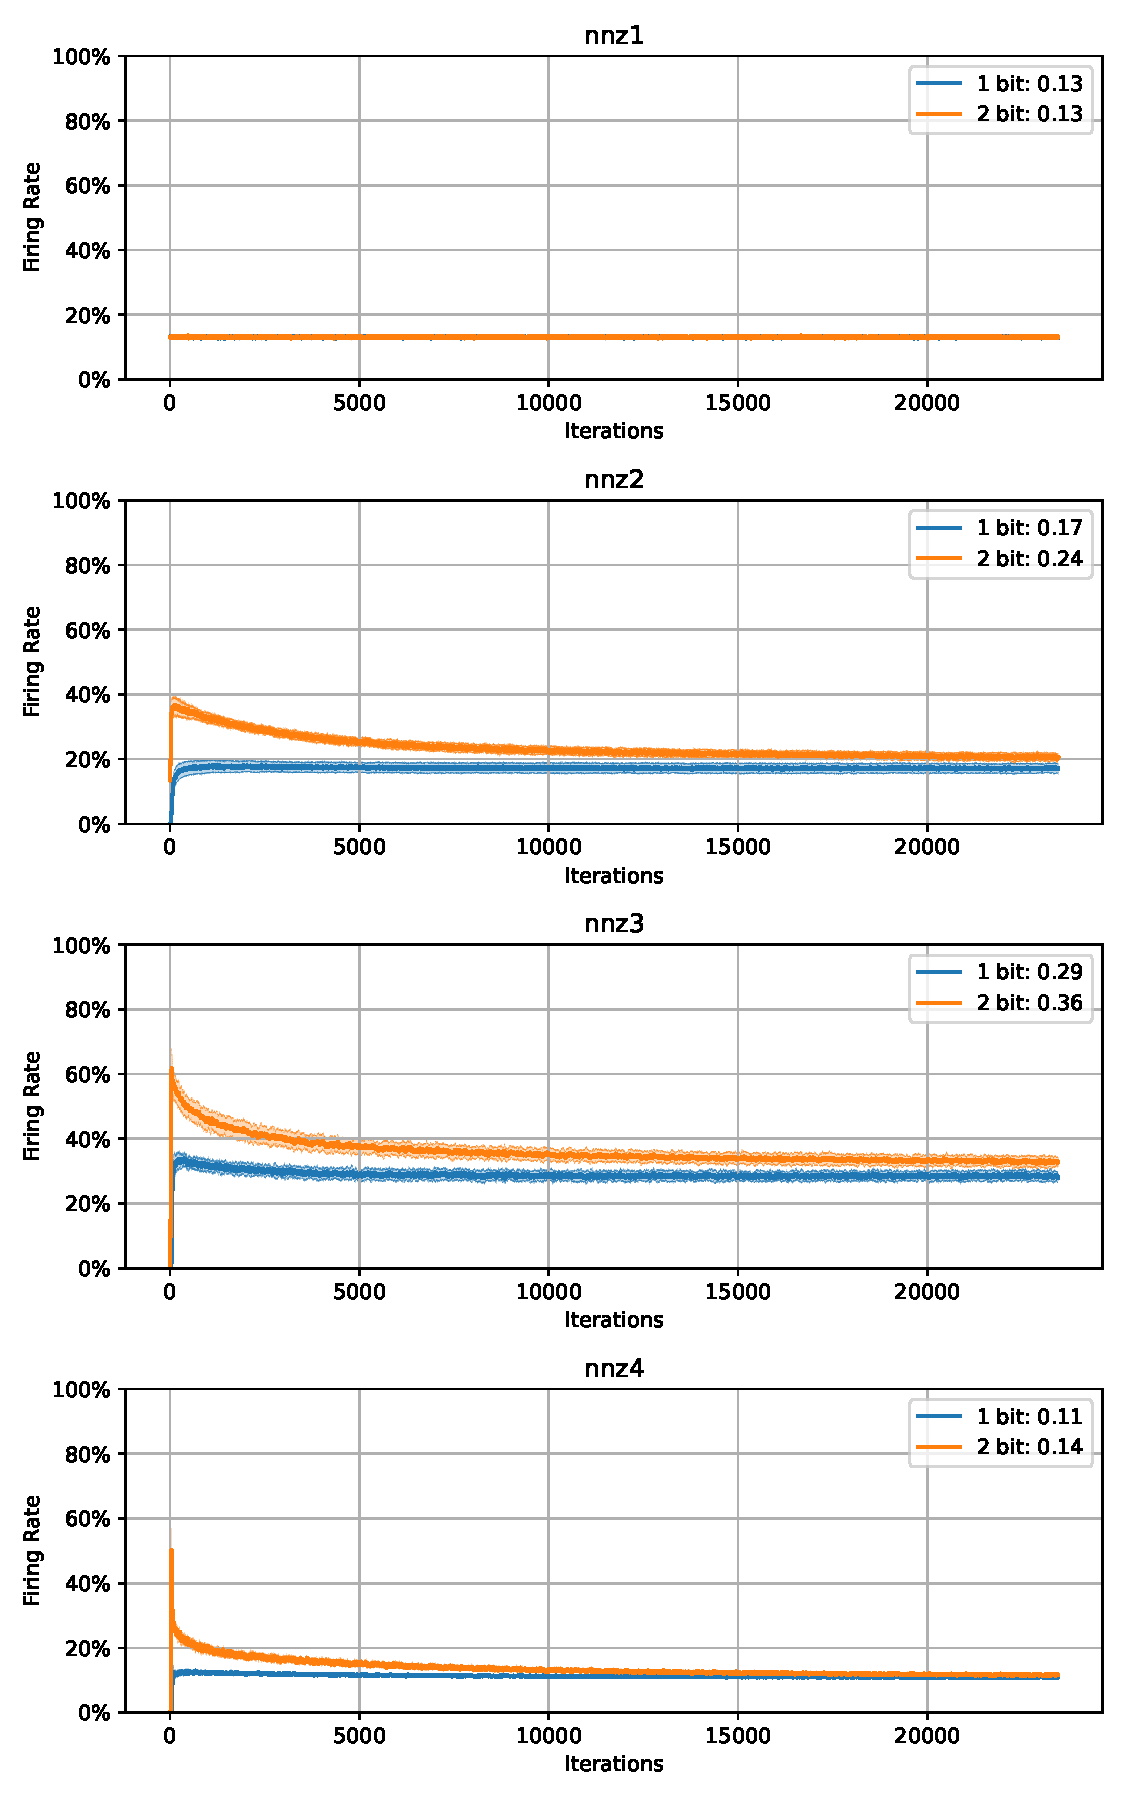
\includegraphics[width=\textwidth]{../firerate/MNIST/plots/mnist_train_firerate.pdf}
                \caption{Firing Rate in Different Positions (Training)}
            \end{subfigure}
            \hfill
            \begin{subfigure}[H]{0.48\textwidth}
                \centering
                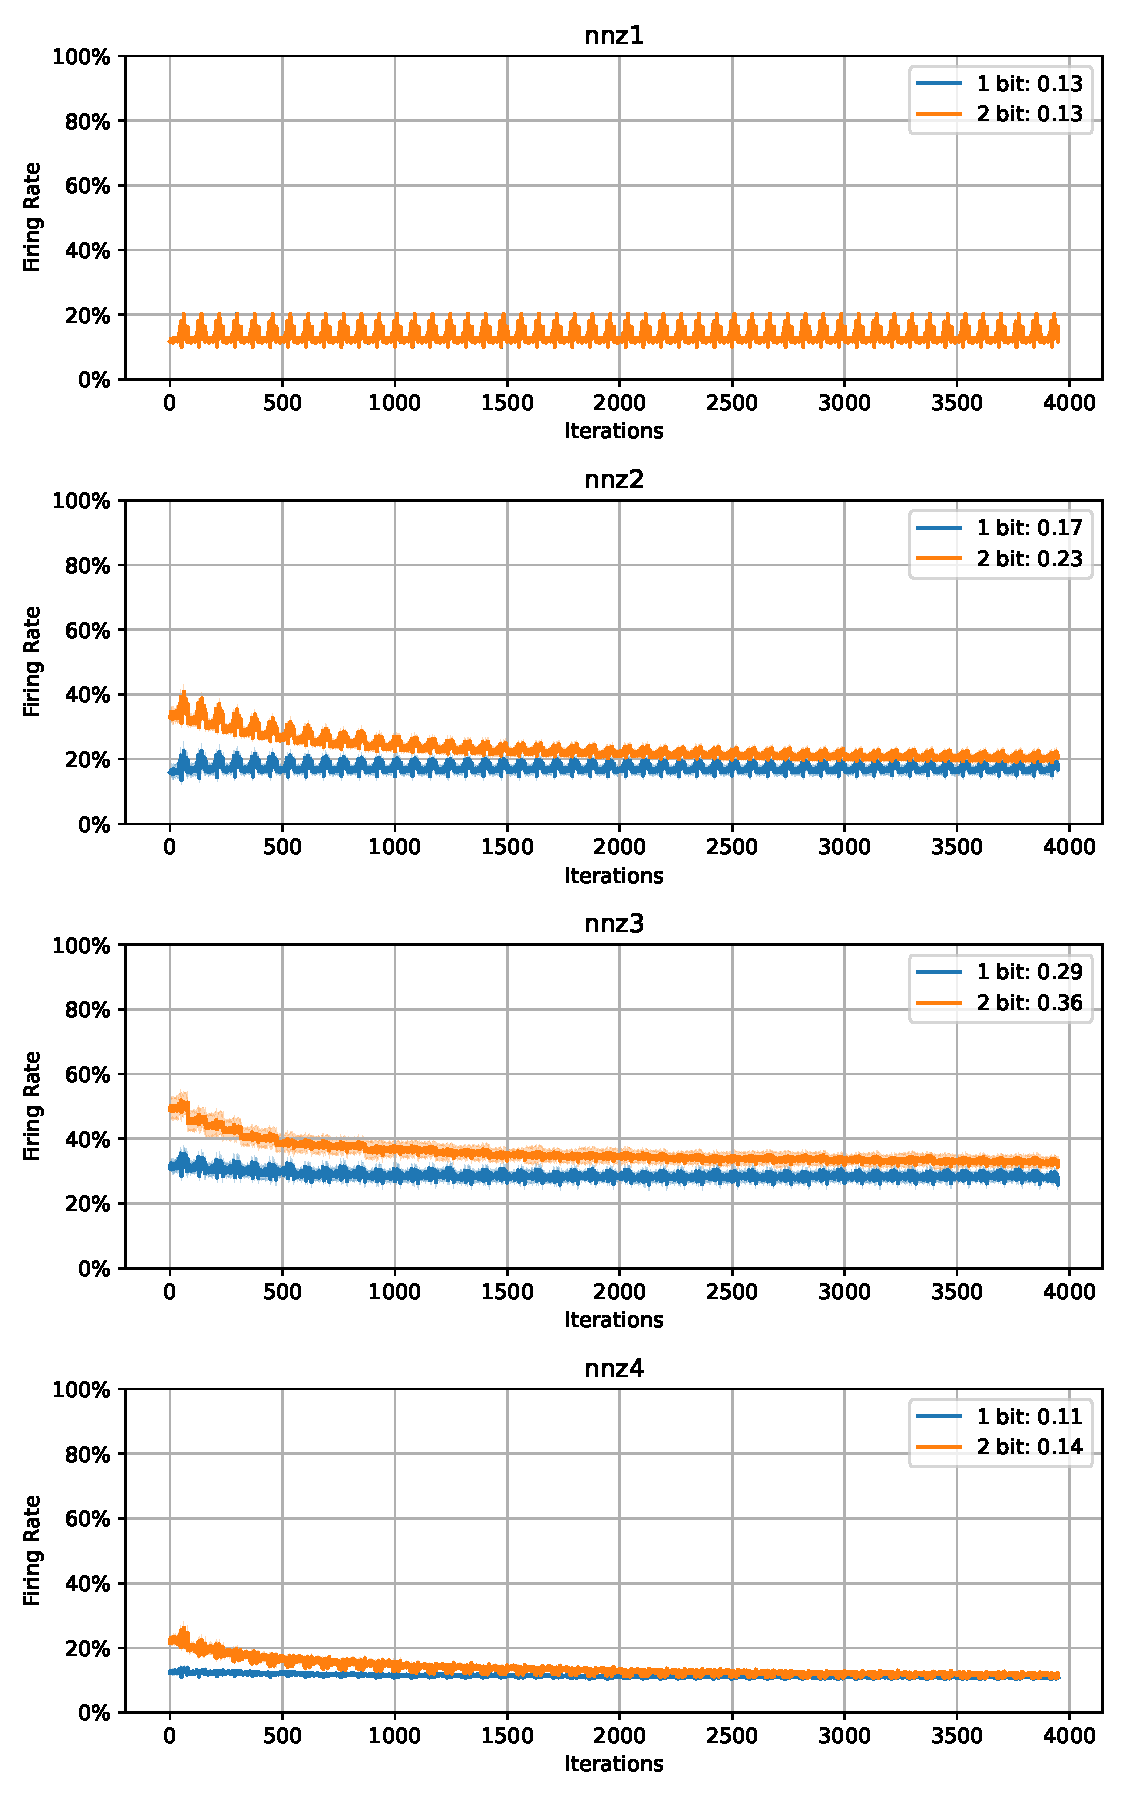
\includegraphics[width=\textwidth]{../firerate/MNIST/plots/mnist_test_firerate.pdf}
                \caption{Firing Rate in Different Positions (Test)}
            \end{subfigure}
            \hfill
            \begin{subfigure}[H]{\textwidth}
                \centering
                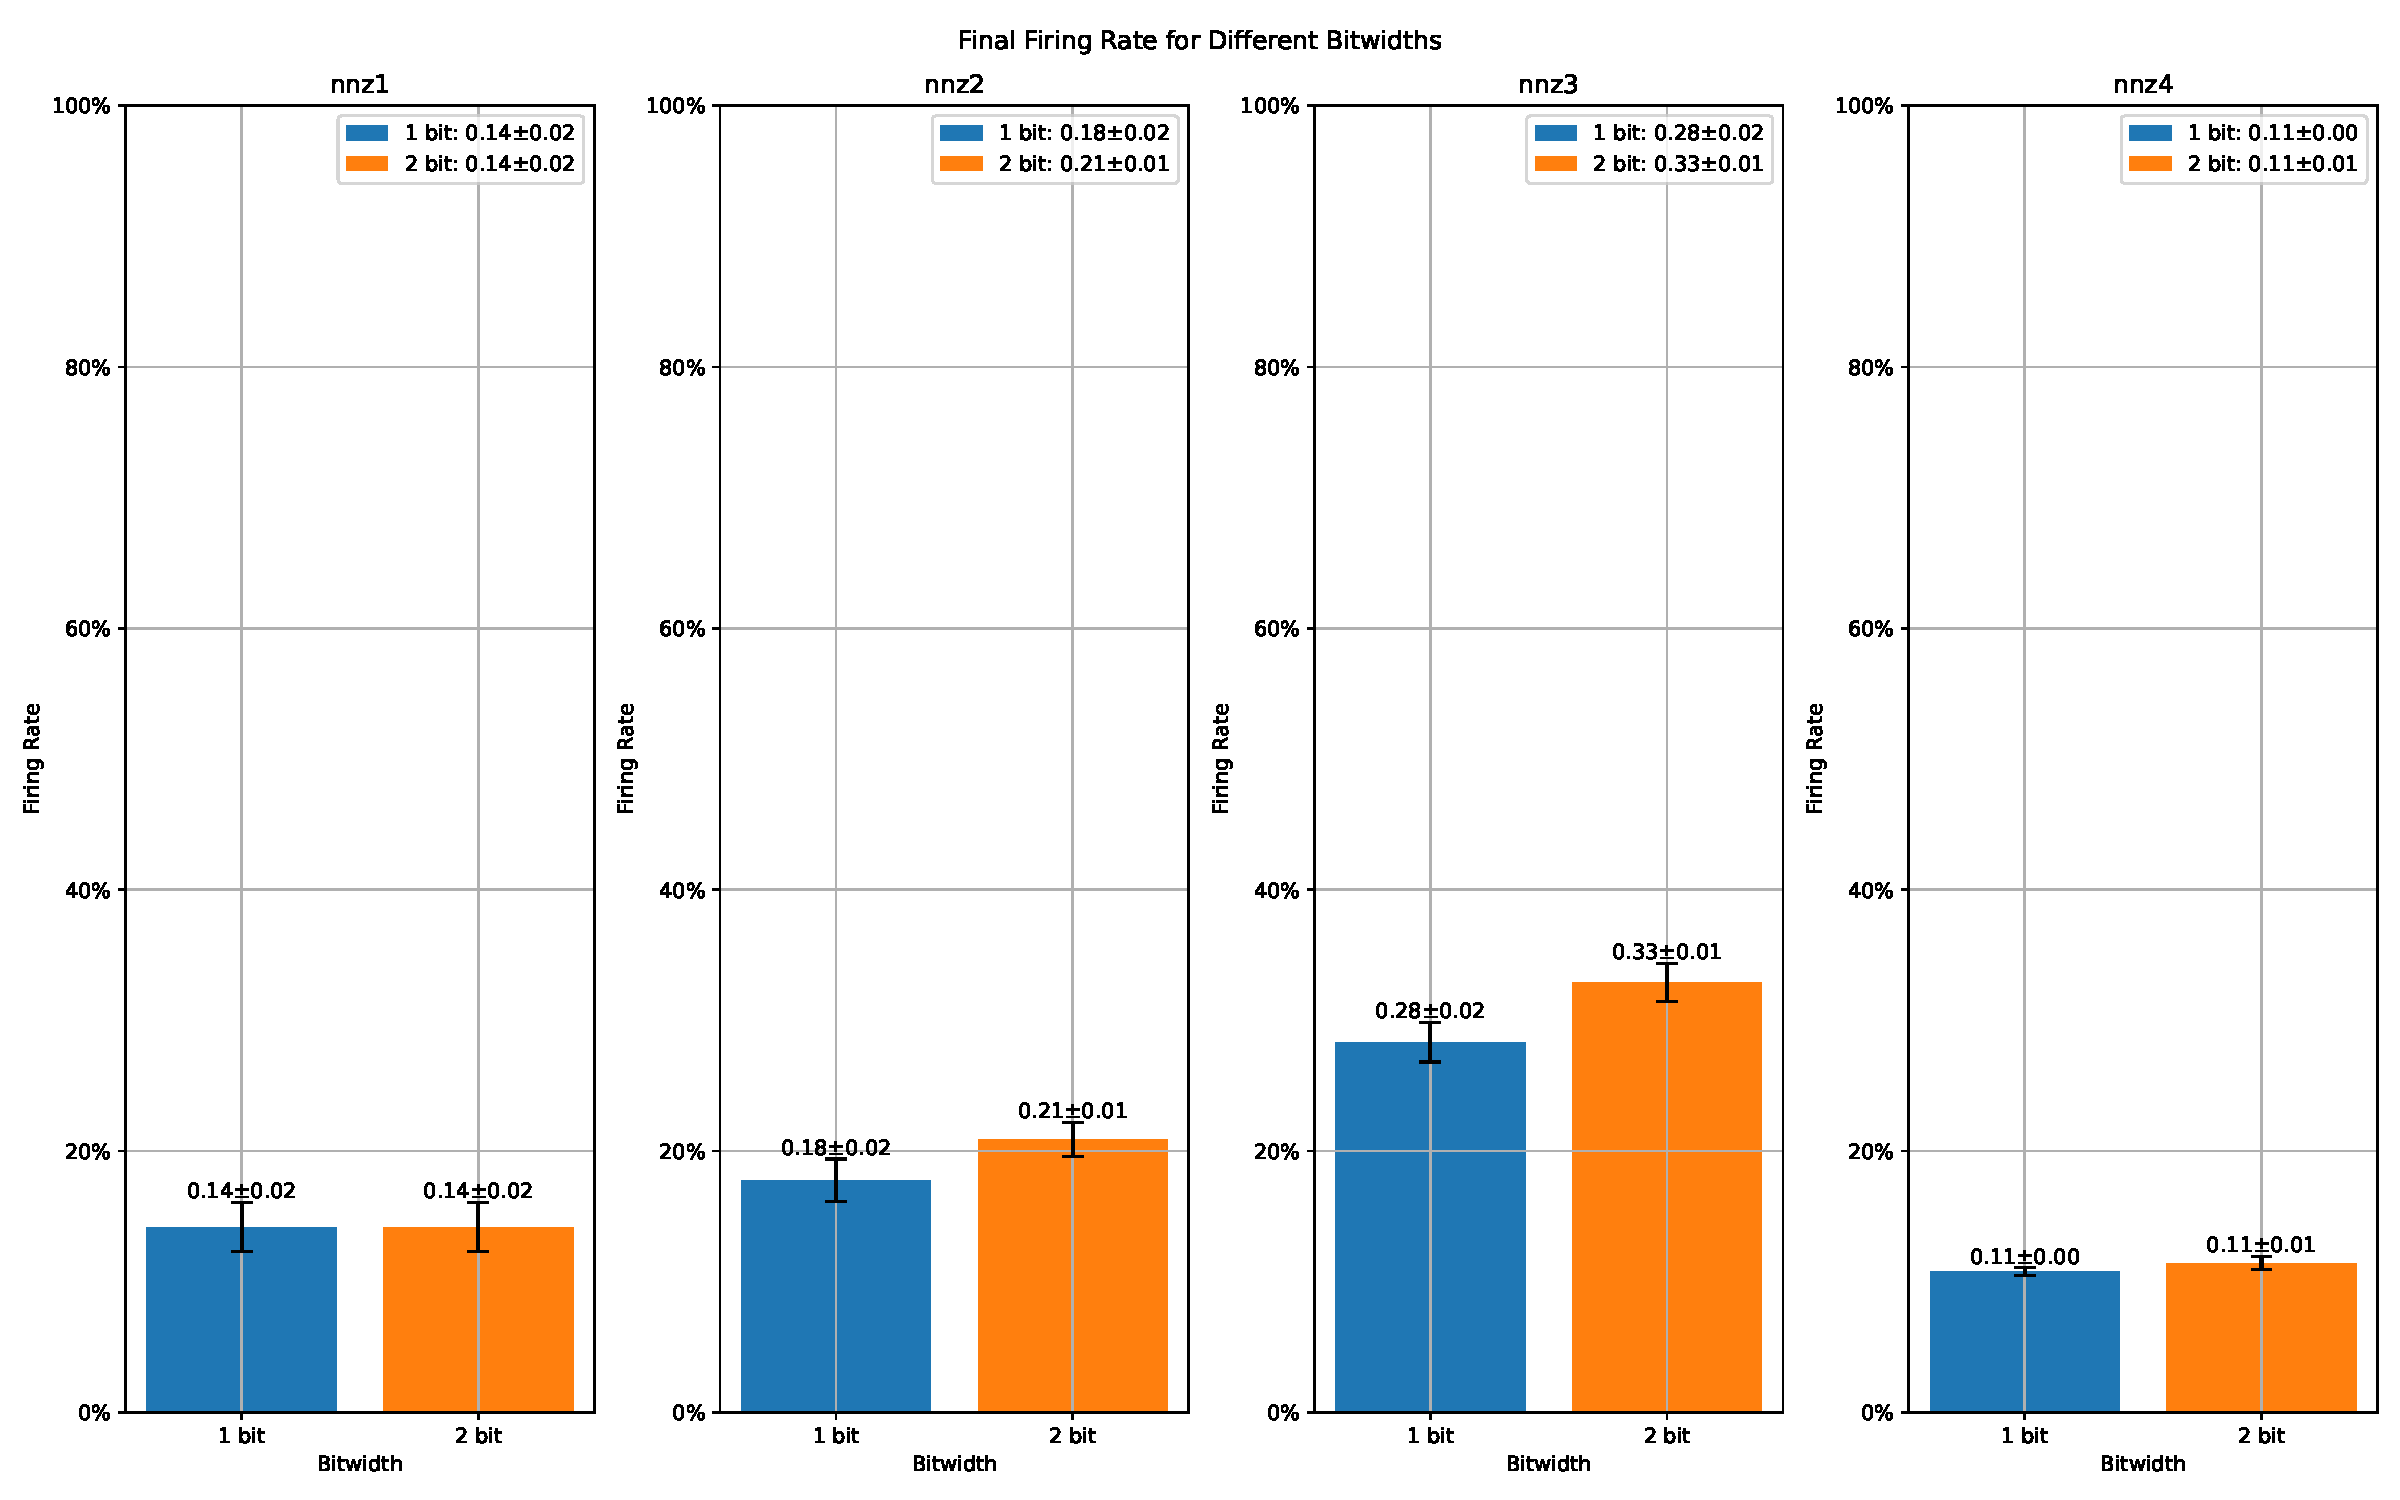
\includegraphics[width=\textwidth]{../firerate/MNIST/plots/mnist_final_firerate.pdf}
                \caption{Firing Rate in Different Positions (Final Test)}
            \end{subfigure}
            \caption{Firing Rate in Different Positions of the MNIST Model}
        \end{figure}

    \section{NMNIST}
    \label{appendix:firerate_nmnist}
        Launch command: 
        \begin{lstlisting}[language=Bash, basicstyle=\small, breaklines=true]
python -m test --N 2 --R 10 --T 10 10 --acc 0.80 --model NMNISTNet --data-path /scratch/zyi/codeSpace/data --dataset NMNIST --batch-size 128 --opt adam --lr 2e-3 --lr-scheduler none --epochs 50 --lr-warmup-epochs 0 --output-dir /scratch/zyi/codeSpace/MultibitSpikes/firerate --mixup-alpha 0.0 --cutmix-alpha 0.0 --label-smoothing 0.0 --disable-amp
        \end{lstlisting}

        \begin{figure}[H]
            \centering
            \begin{subfigure}[H]{0.48\textwidth}
                \centering
                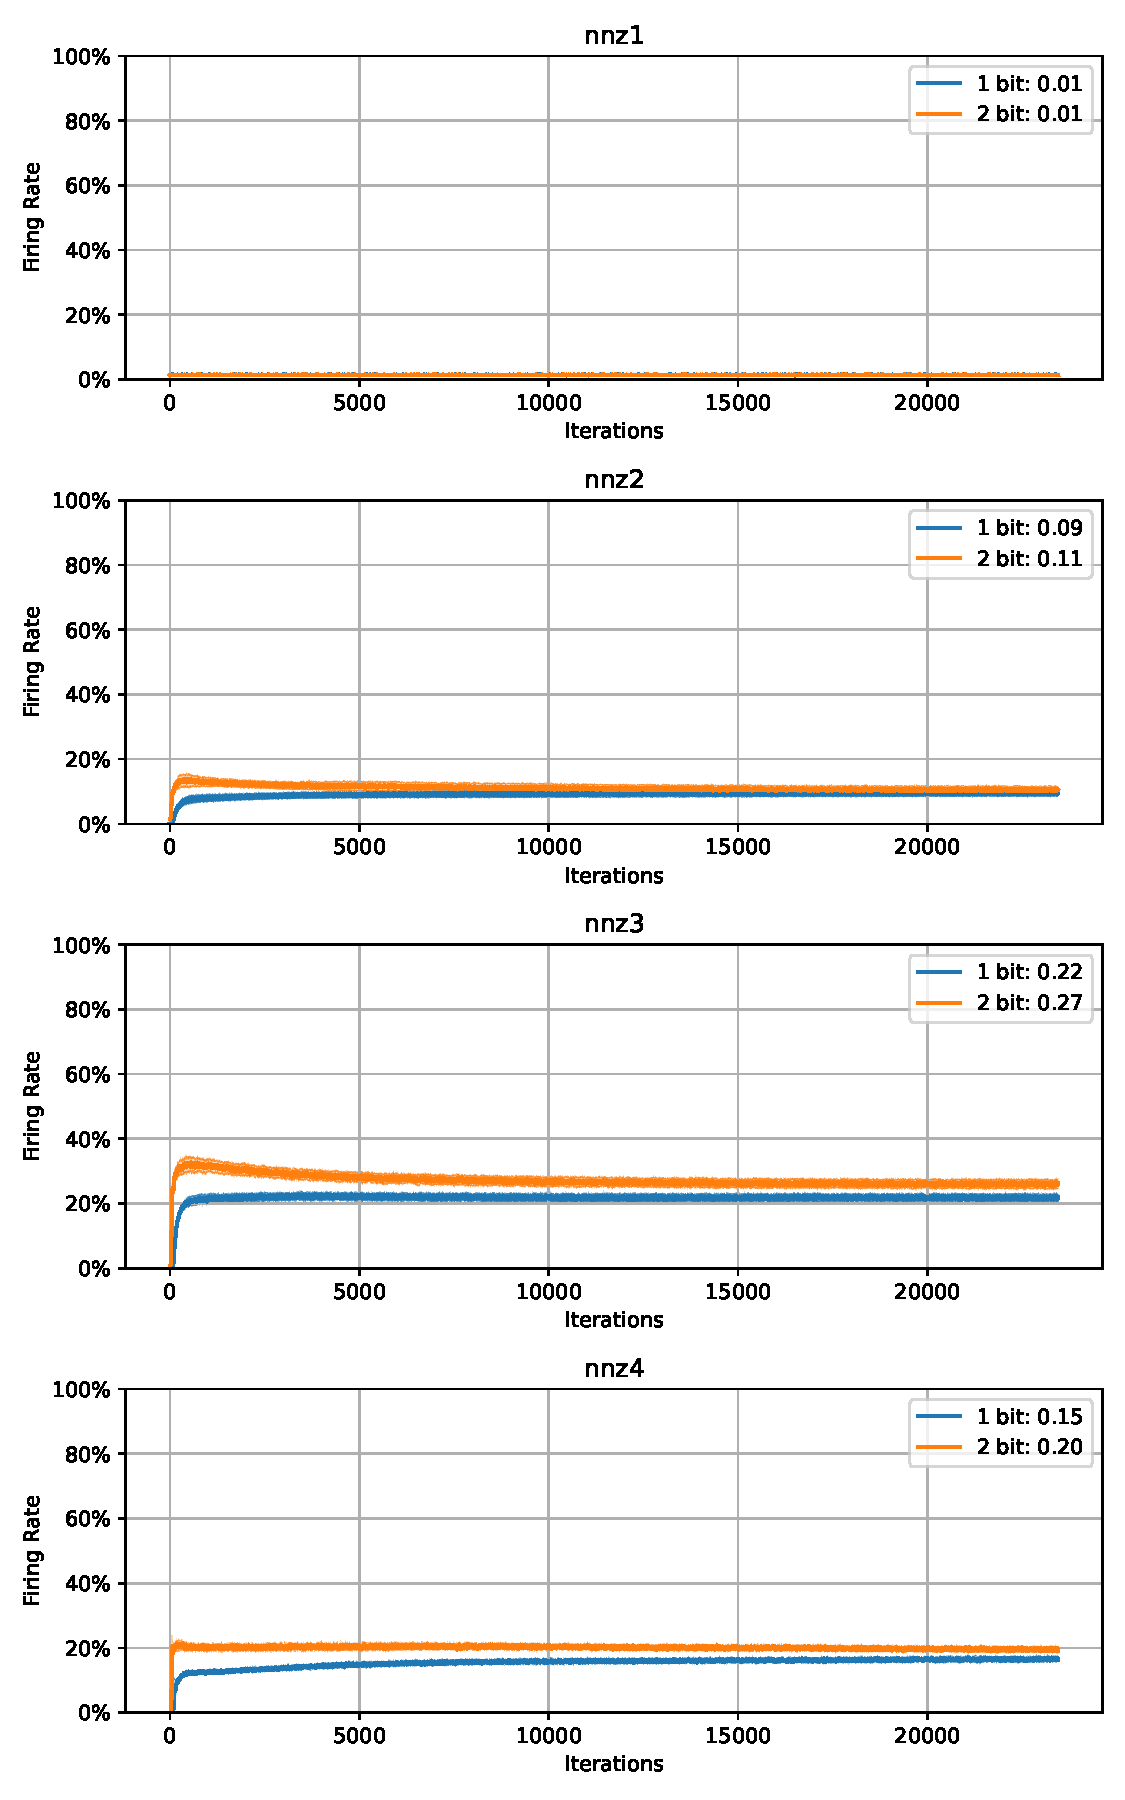
\includegraphics[width=\textwidth]{../firerate/NMNIST/plots/nmnist_train_firerate.pdf}
                \caption{Firing Rate in Different Positions (Training)}
            \end{subfigure}
            \hfill
            \begin{subfigure}[H]{0.48\textwidth}
                \centering
                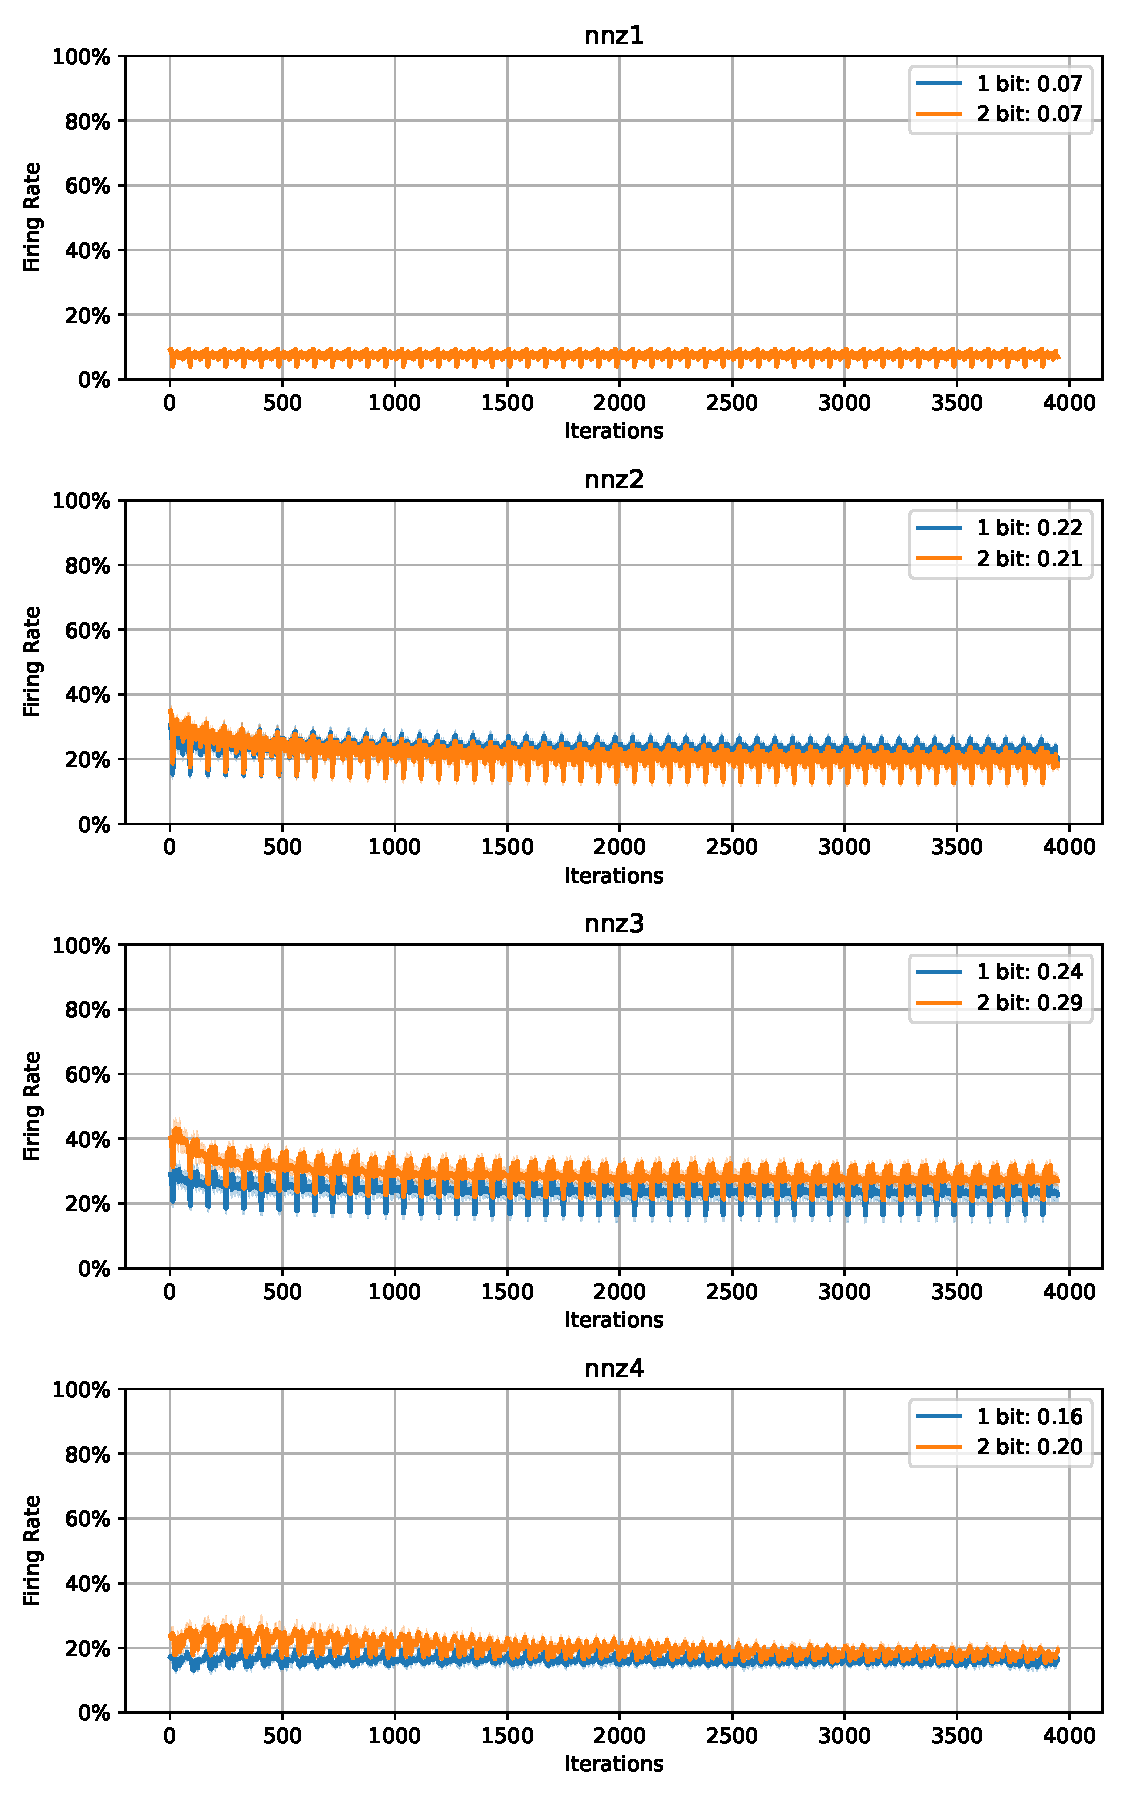
\includegraphics[width=\textwidth]{../firerate/NMNIST/plots/nmnist_test_firerate.pdf}
                \caption{Firing Rate in Different Positions (Test)}
            \end{subfigure}
            \hfill
            \begin{subfigure}[H]{\textwidth}
                \centering
                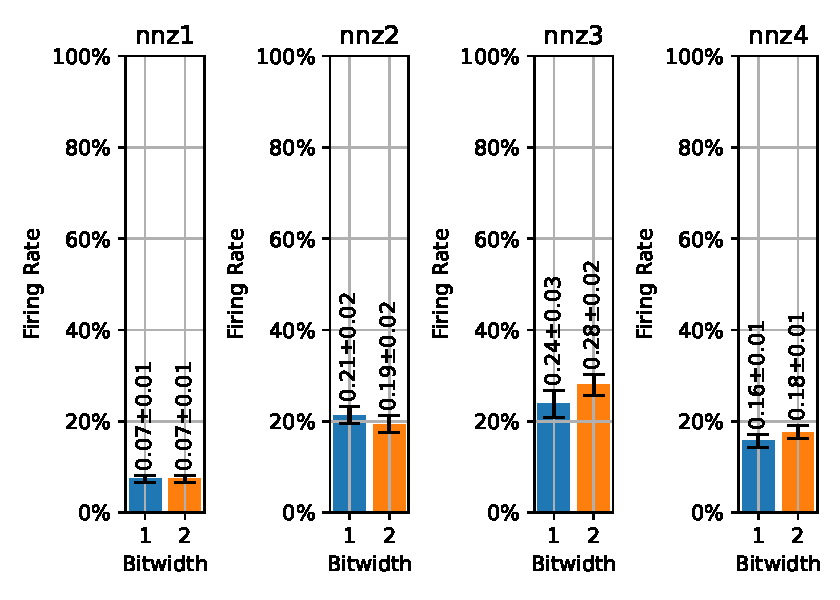
\includegraphics[width=\textwidth]{../firerate/NMNIST/plots/nmnist_final_firerate.pdf}
                \caption{Firing Rate in Different Positions (Final Test)}
            \end{subfigure}
            \caption{Firing Rate in Different Positions of the NMNIST Model}
        \end{figure}

    \section{DVS Gesture}
    \label{appendix:firerate_dvs_gesture}
        Launch command: 
        \begin{lstlisting}[language=Bash, basicstyle=\small, breaklines=true]
python -m test --N 2 --R 10 --T 10 10 --acc 0.80 --model DVSGestureNet --data-path /scratch/zyi/codeSpace/data --dataset DVSGesture --batch-size 128 --opt adam --lr 1e-3 --lr-scheduler cosa --epochs 200 --lr-warmup-epochs 0 --output-dir /scratch/zyi/codeSpace/MultibitSpikes/firerate
        \end{lstlisting}

        The results of experiments on DVS Gesture dataset are the only exception against our conclusion. We suspect that our model is overfitting the training data such that the multi-bit spike train model and the 1-bit spike train model are not generalizing the same way. 

        \begin{figure}[H]
            \centering
            \begin{subfigure}[H]{0.48\textwidth}
                \centering
                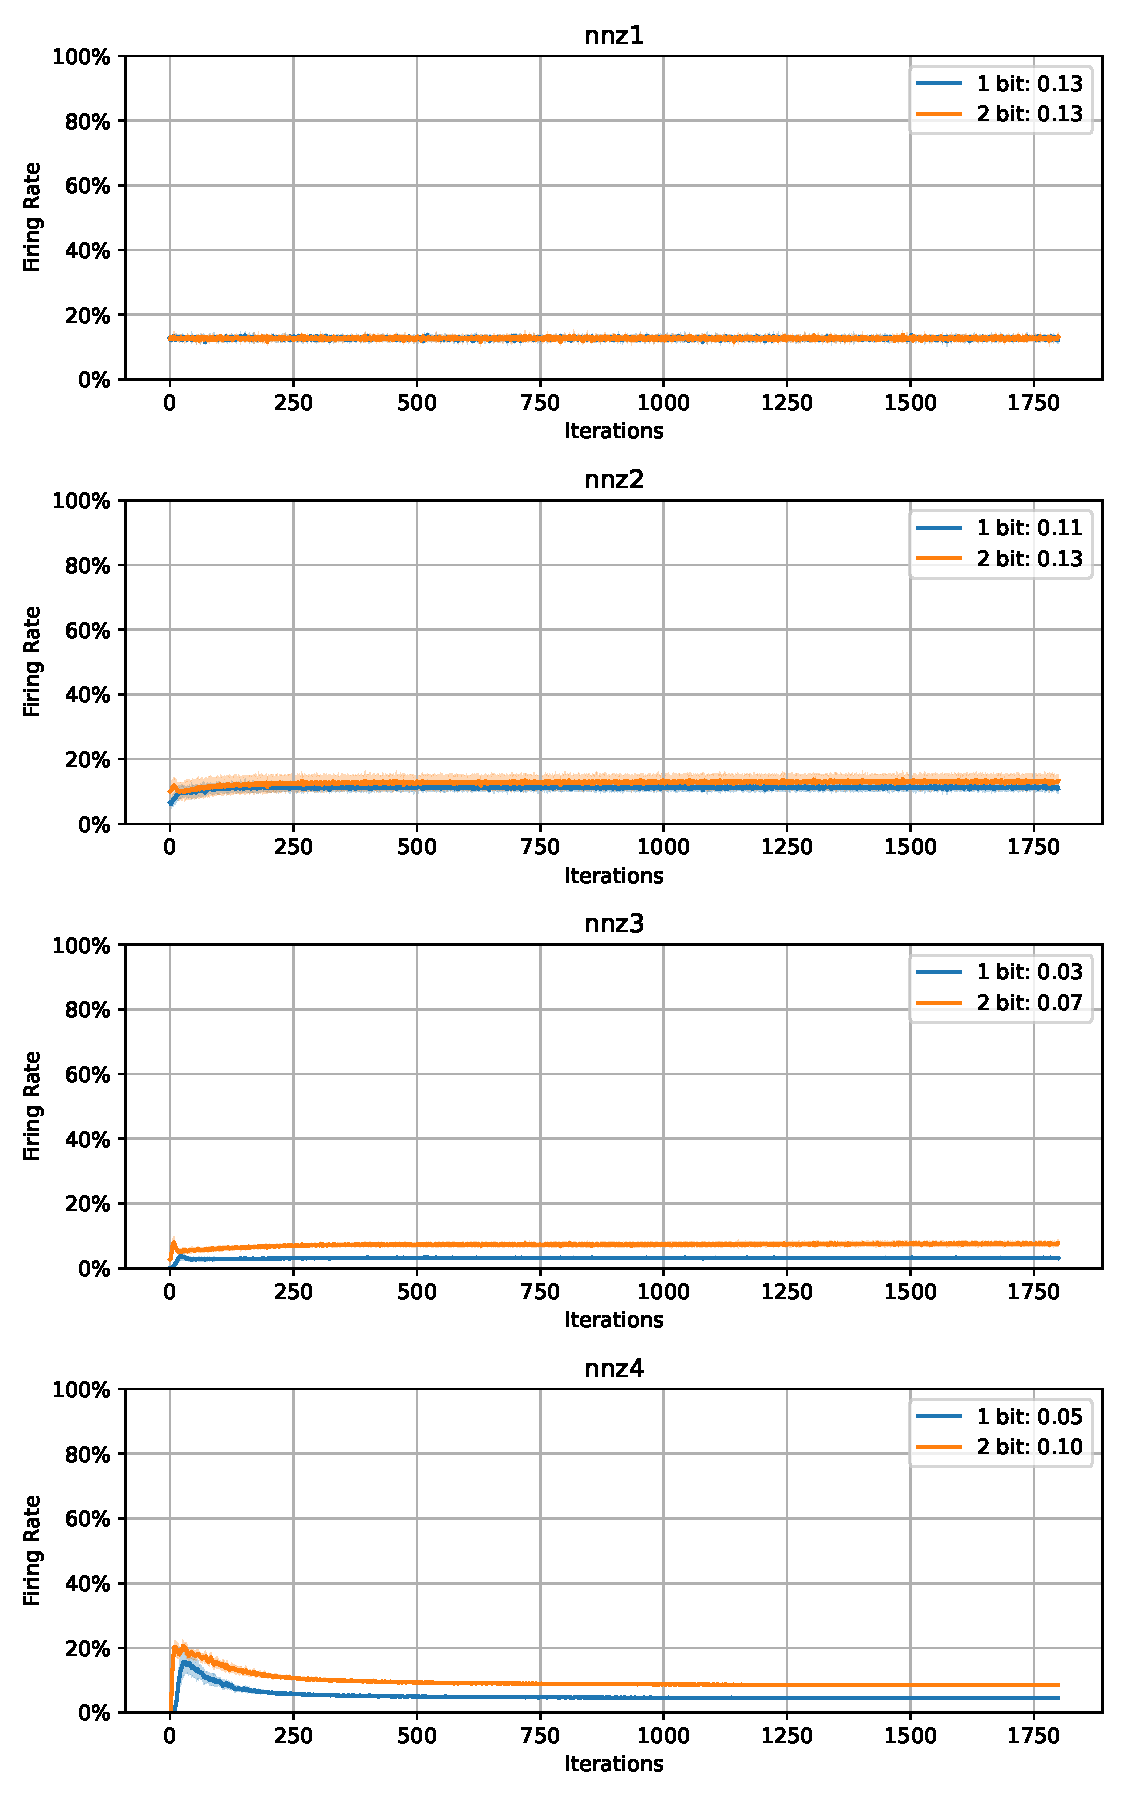
\includegraphics[width=\textwidth]{../firerate/DVSGesture/plots/dvsgesture_train_firerate.pdf}
                \caption{Firing Rate in Different Positions (Training)}
            \end{subfigure}
            \hfill
            \begin{subfigure}[H]{0.48\textwidth}
                \centering
                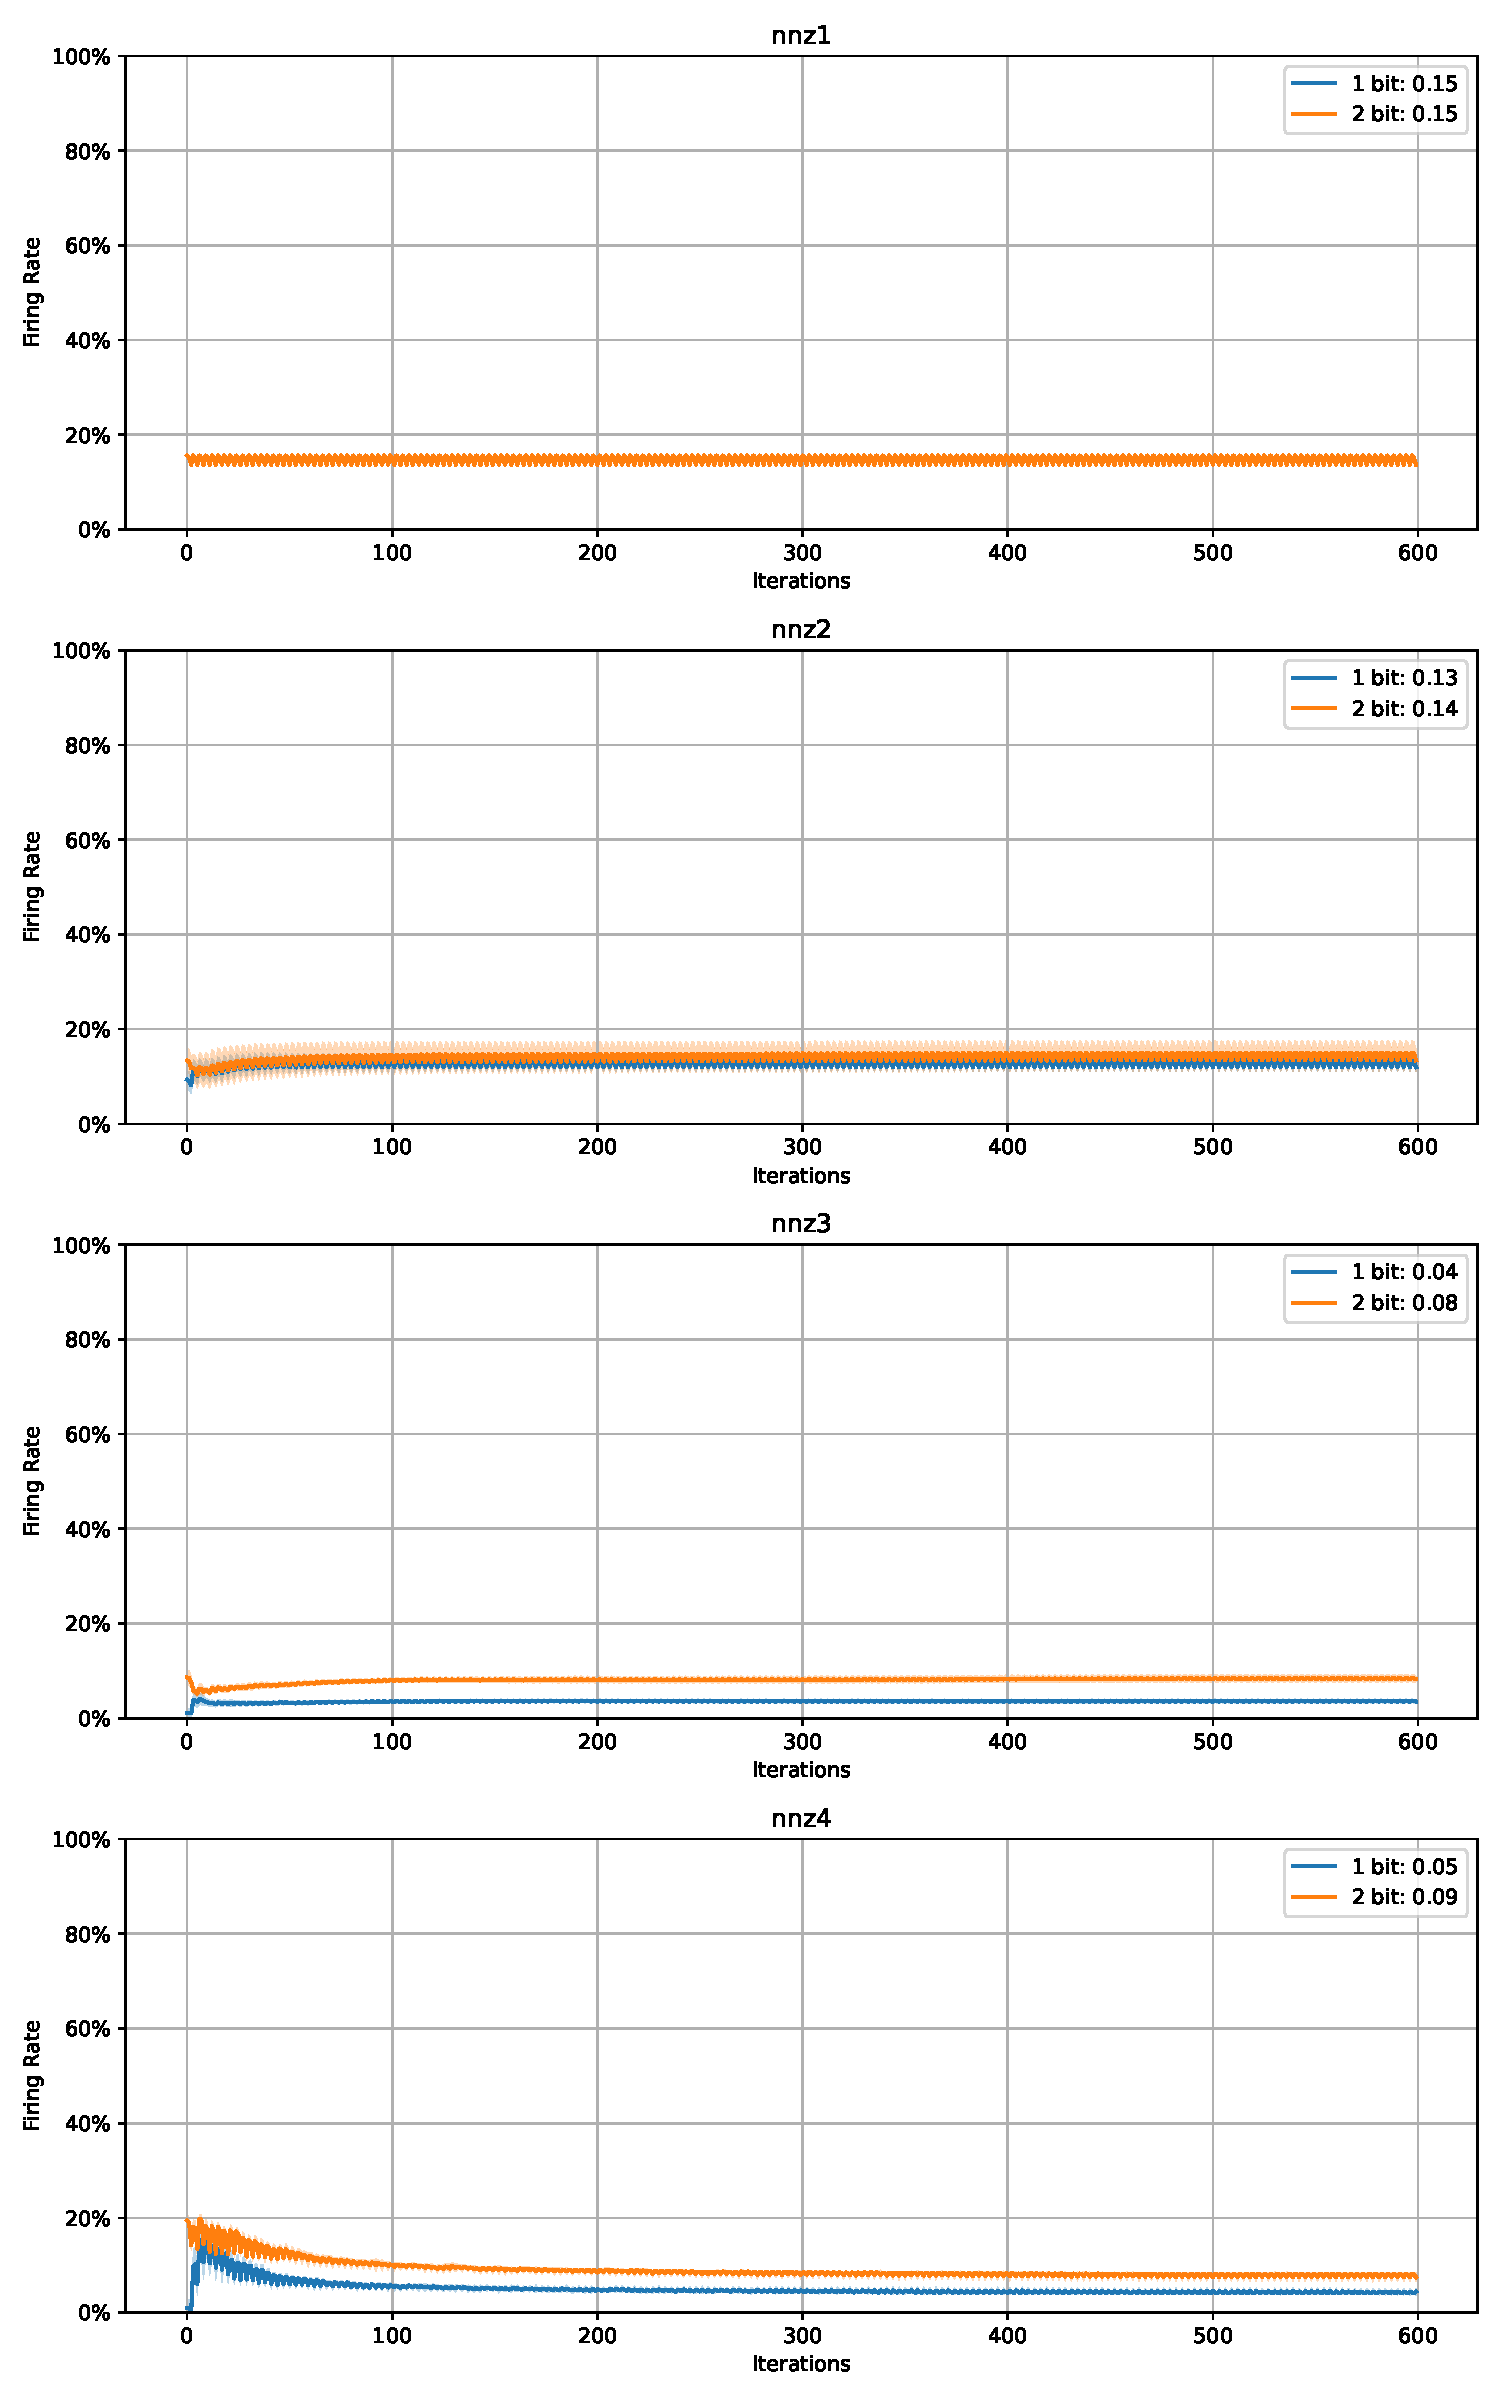
\includegraphics[width=\textwidth]{../firerate/DVSGesture/plots/dvsgesture_test_firerate.pdf}
                \caption{Firing Rate in Different Positions (Test)}
            \end{subfigure}
            \hfill
            \begin{subfigure}[H]{\textwidth}
                \centering
                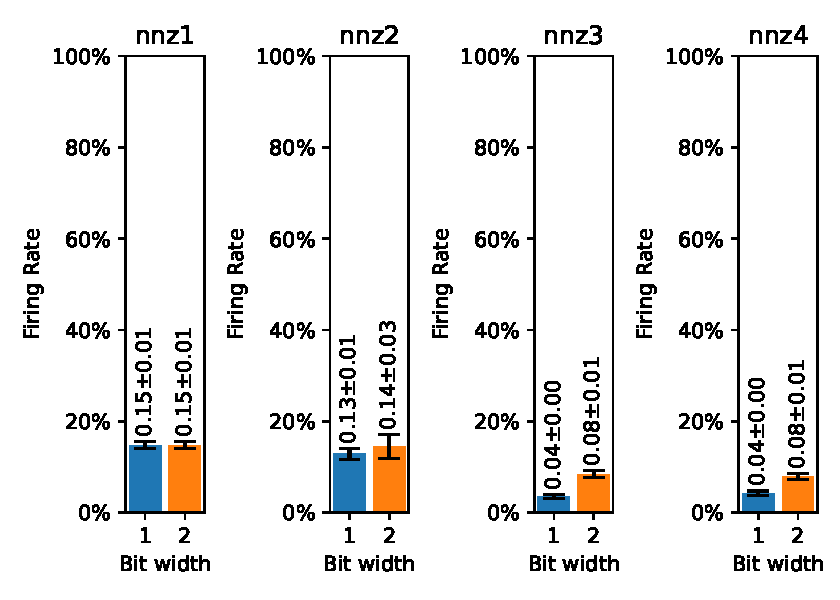
\includegraphics[width=\textwidth]{../firerate/DVSGesture/plots/dvsgesture_final_firerate.pdf}
                \caption{Firing Rate in Different Positions (Final Test)}
            \end{subfigure}
            \caption{Firing Rate in Different Positions of the DVS Gesture Model}
        \end{figure}

    \section{CIFAR-10}
    \label{appendix:firerate_cifar10}
        Launch command: 
        \begin{lstlisting}[language=Bash, basicstyle=\small, breaklines=true]
python -m test --N 2 --R 5 --T 10 10 --acc 0.80 --model CIFAR10Net --data-path /scratch/zyi/codeSpace/data --dataset CIFAR10 --batch-size 128 --opt adam --lr 1e-5 --lr-scheduler none --epochs 1000 --lr-warmup-epochs 0 --output-dir /scratch/zyi/codeSpace/MultibitSpikes/firerate
        \end{lstlisting}

        Here we use learning rate schedulers to accelerate the convergence of the models. Although the models can reach a high accuracy faster, the multi-bit spike train model suffers from the high learning rate from time to time. 

        \begin{figure}[H]
            \centering
            \begin{subfigure}[H]{0.48\textwidth}
                \centering
                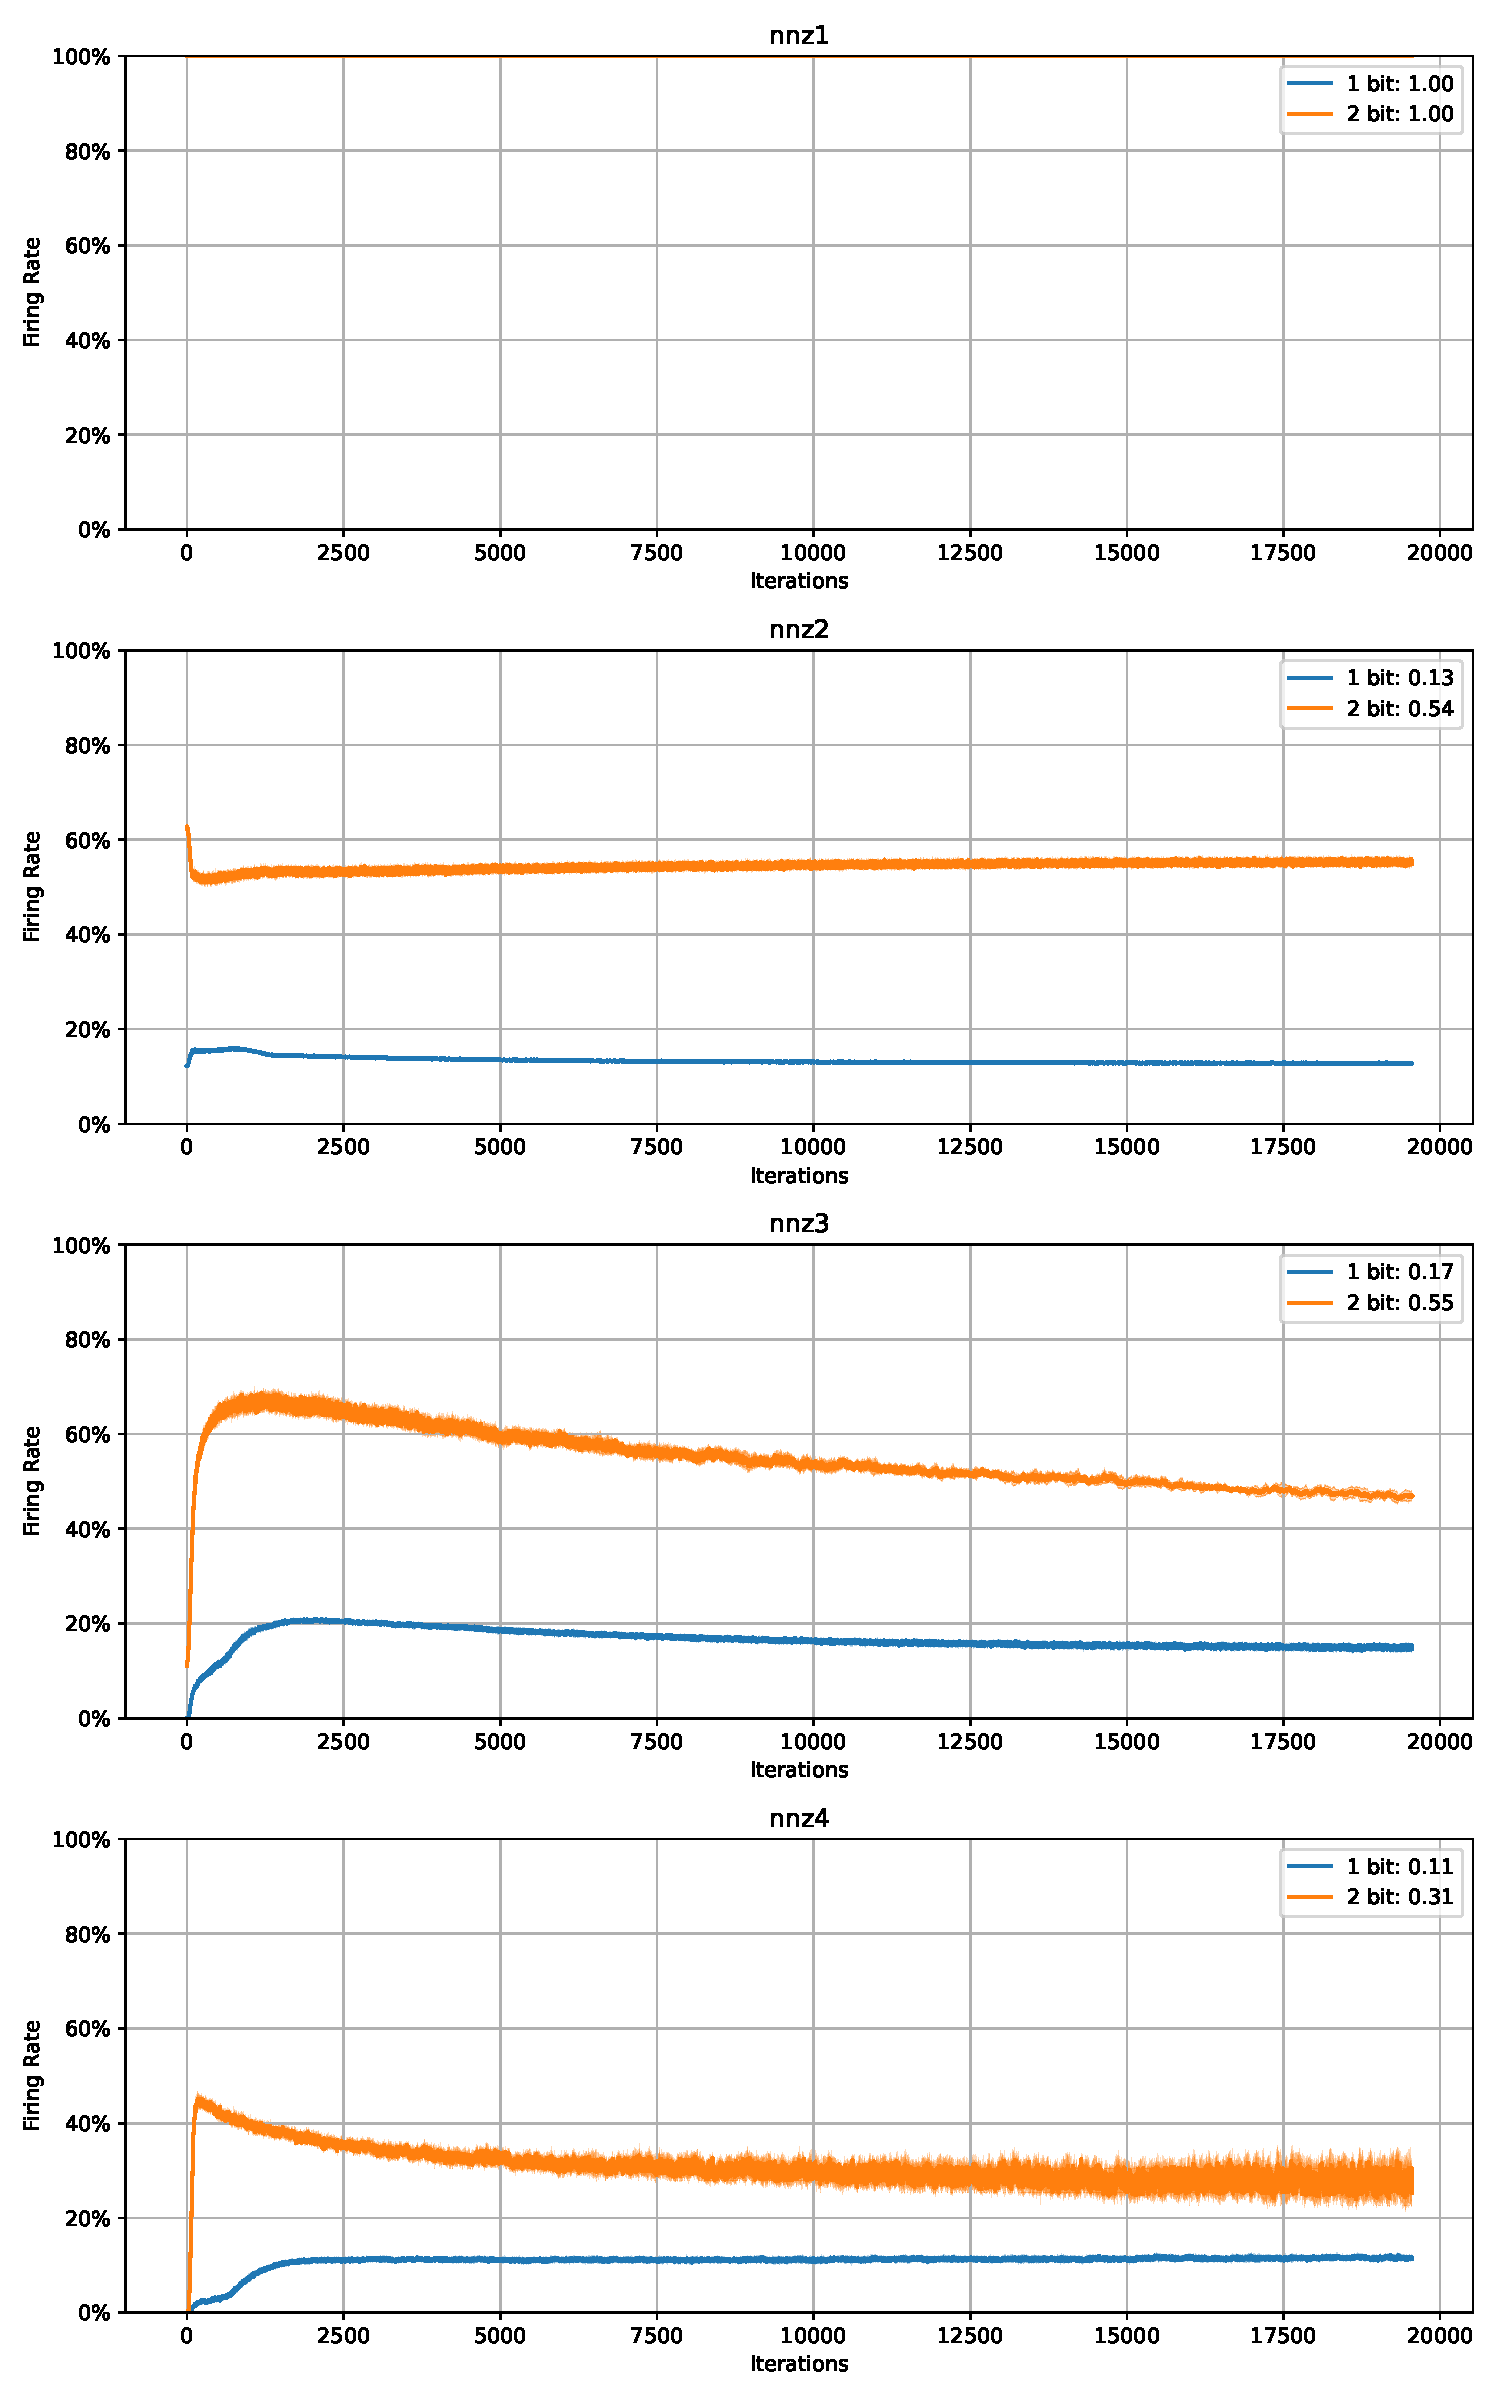
\includegraphics[width=\textwidth]{../firerate/CIFAR10/plots/cifar10_train_firerate.pdf}
                \caption{Firing Rate in Different Positions (Training)}
            \end{subfigure}
            \hfill
            \begin{subfigure}[H]{0.48\textwidth}
                \centering
                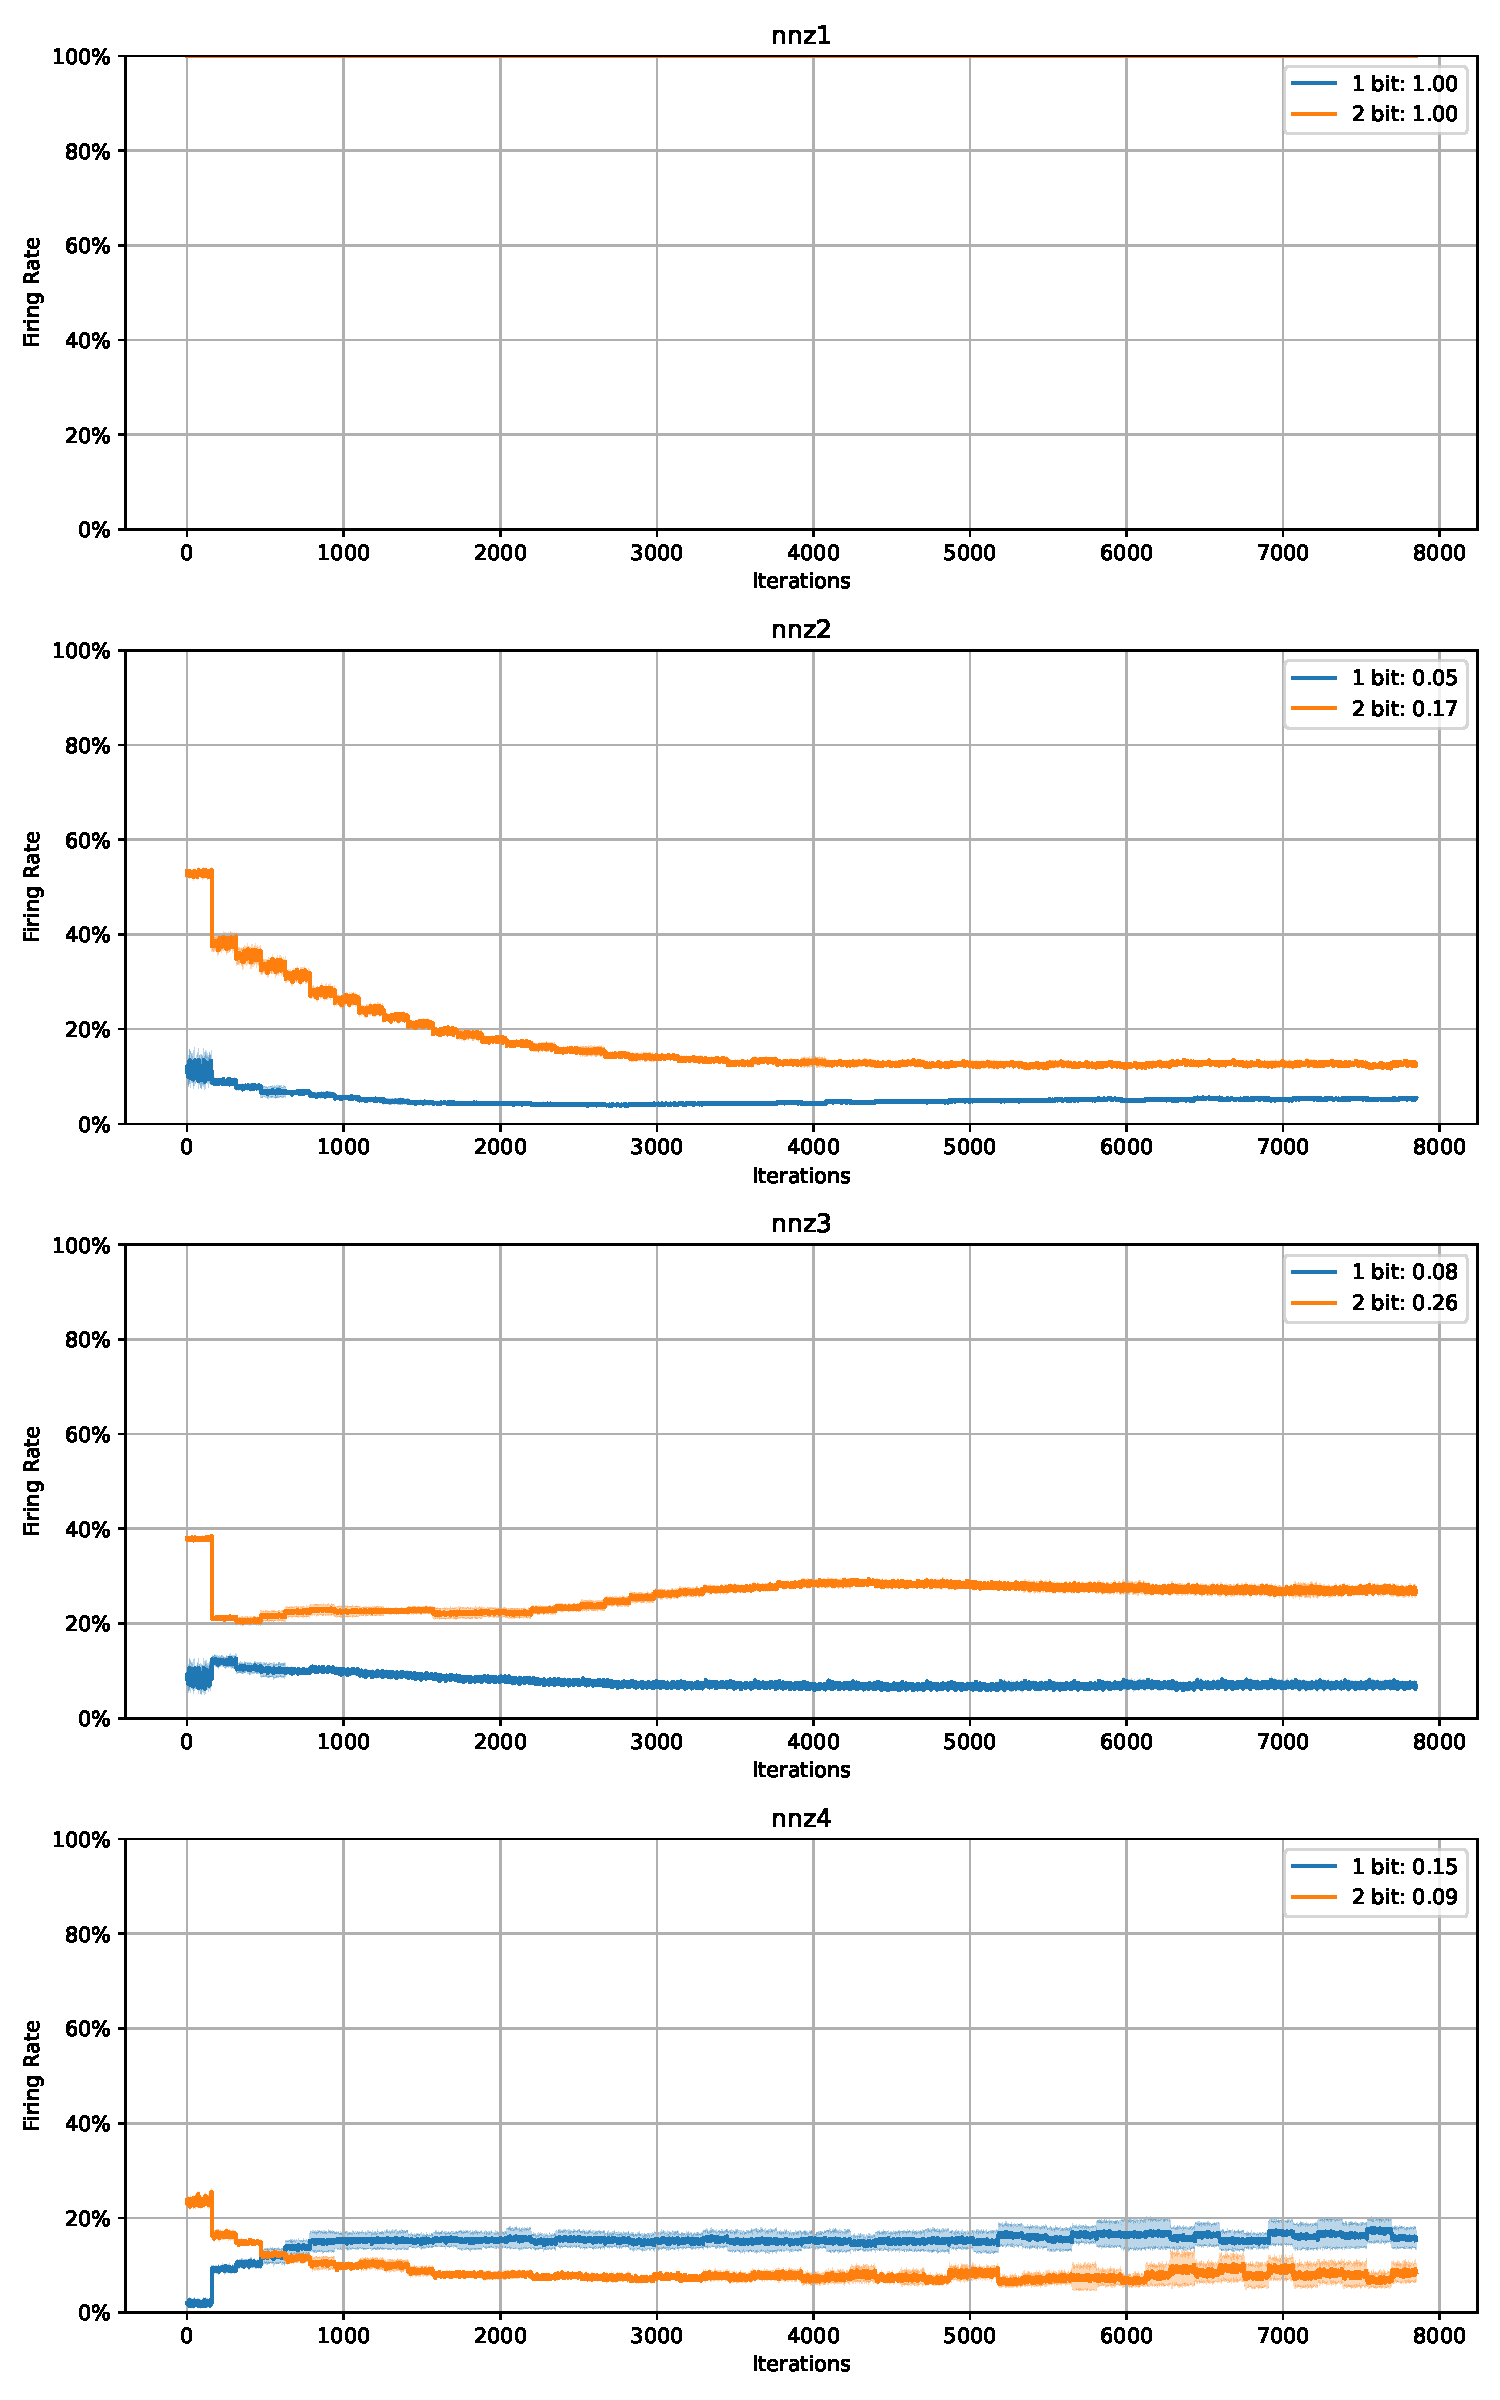
\includegraphics[width=\textwidth]{../firerate/CIFAR10/plots/cifar10_test_firerate.pdf}
                \caption{Firing Rate in Different Positions (Test)}
            \end{subfigure}
            \hfill
            \begin{subfigure}[H]{\textwidth}
                \centering
                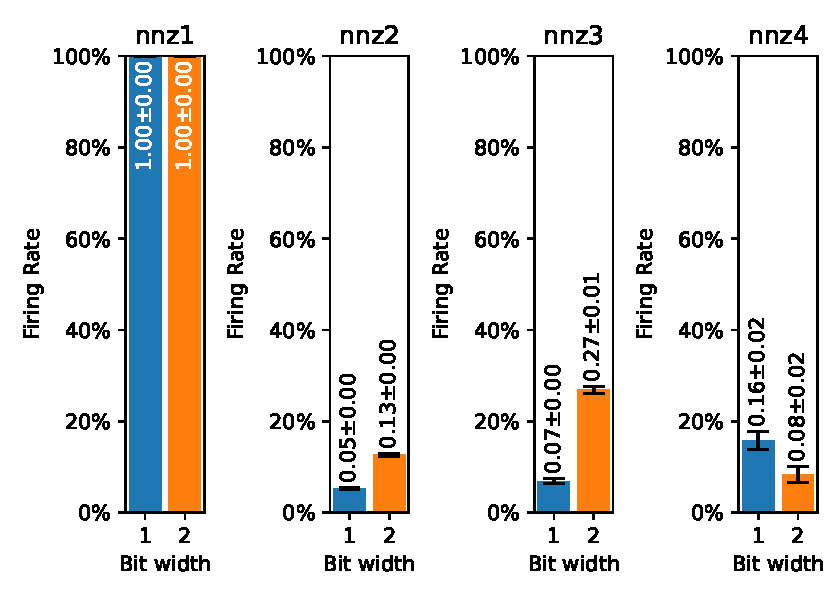
\includegraphics[width=\textwidth]{../firerate/CIFAR10/plots/cifar10_final_firerate.pdf}
                \caption{Firing Rate in Different Positions (Final Test)}
            \end{subfigure}
            \caption{Firing Rate in Different Positions of the CIFAR-10 Model}
        \end{figure}


\chapter{Energy Consumption Estimation}
\label{appendix:energy}

\section{Training Energy Consumption Estimation on GPUs}
\label{appendix:energy_gpu}

    \subsection{Fashion MNIST}
    \label{appendix:energy_gpu_fashion_mnist}
        Launch command: Same as in Appendix \ref{appendix:accuracy_curves_fashion_mnist}

        \begin{figure}[H]
            \centering
            \begin{subfigure}[H]{0.495\textwidth}
                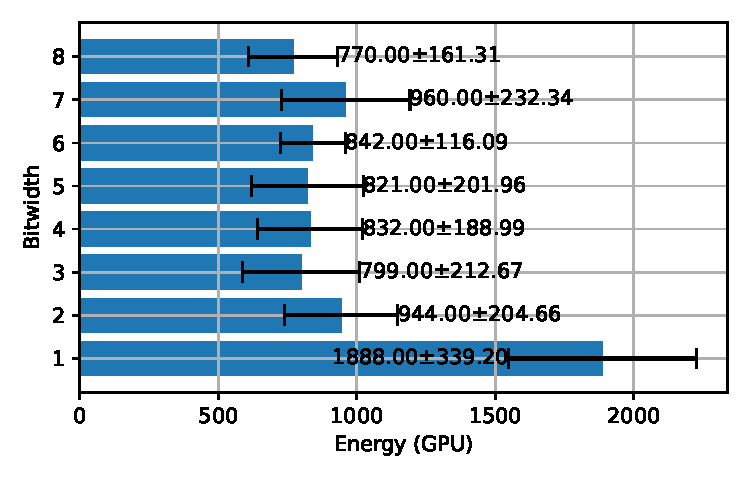
\includegraphics[width=\textwidth]{../standard/FashionMNIST/plots/fashionmnist_train_energy_gpu_horizontal.pdf}
                \caption{Energy Consumption Estimation, Unit in Constant $c$}
            \end{subfigure}
            \hfill
            \begin{subfigure}[H]{0.495\textwidth}
                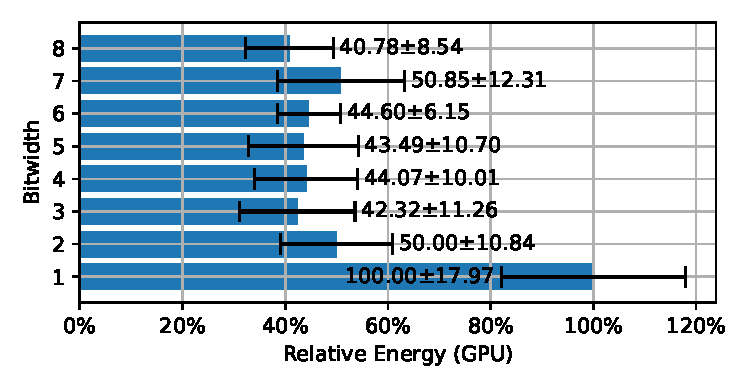
\includegraphics[width=\textwidth]{../standard/FashionMNIST/plots/fashionmnist_train_relative_energy_gpu_horizontal.pdf}
                \caption{Normalized Energy Consumption Estimation Relative to 1-bit Spike Train Model}
            \end{subfigure}
            \caption{Training Energy Consumption Estimation on GPUs for Fashion MNIST Dataset}
        \end{figure}

    \subsection{MNIST}
    \label{appendix:energy_gpu_mnist}
        Launch command: Same as in Appendix \ref{appendix:accuracy_curves_mnist}

        \begin{figure}[H]
            \centering
            \begin{subfigure}[H]{0.48\textwidth}
                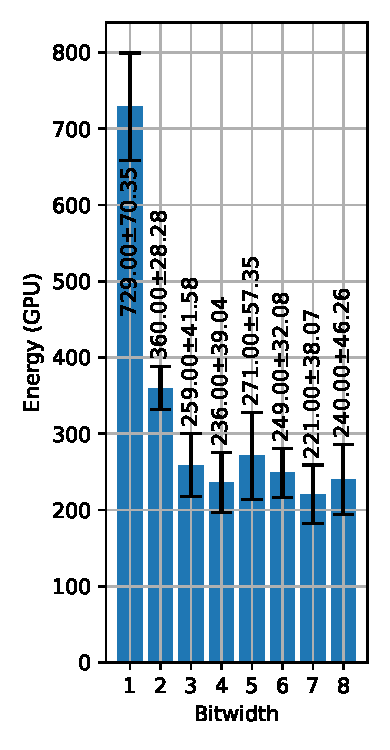
\includegraphics[width=\textwidth]{../standard/MNIST/plots/mnist_train_energy_gpu.pdf}
                \caption{Energy Consumption Estimation, Unit in Constant $c$}
            \end{subfigure}
            \hfill
            \begin{subfigure}[H]{0.48\textwidth}
                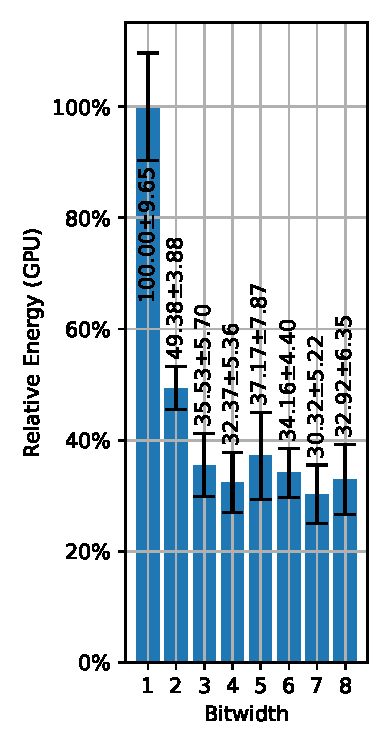
\includegraphics[width=\textwidth]{../standard/MNIST/plots/mnist_train_relative_energy_gpu.pdf}
                \caption{Normalized Energy Consumption Estimation Relative to 1-bit Spike Train Model}
            \end{subfigure}
            \caption{Training Energy Consumption Estimation on GPUs for MNIST Dataset}
        \end{figure}

    \subsection{NMNIST}
    \label{appendix:energy_gpu_nmnist}
        Launch command: Same as in Appendix \ref{appendix:accuracy_curves_nmnist}

        \begin{figure}[H]
            \centering
            \begin{subfigure}[H]{0.48\textwidth}
                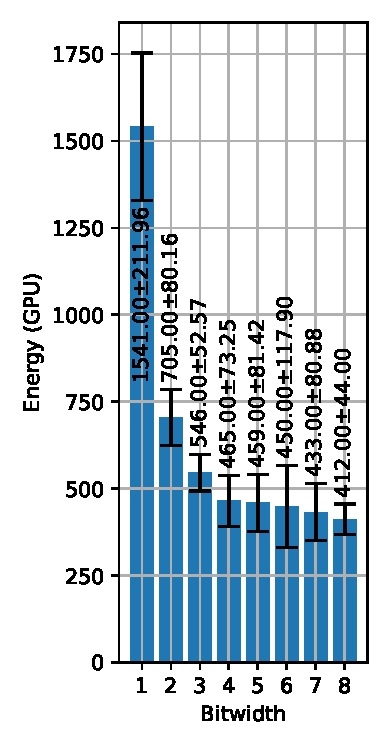
\includegraphics[width=\textwidth]{../standard/NMNIST/plots/nmnist_train_energy_gpu.pdf}
                \caption{Energy Consumption Estimation, Unit in Constant $c$}
            \end{subfigure}
            \hfill
            \begin{subfigure}[H]{0.48\textwidth}
                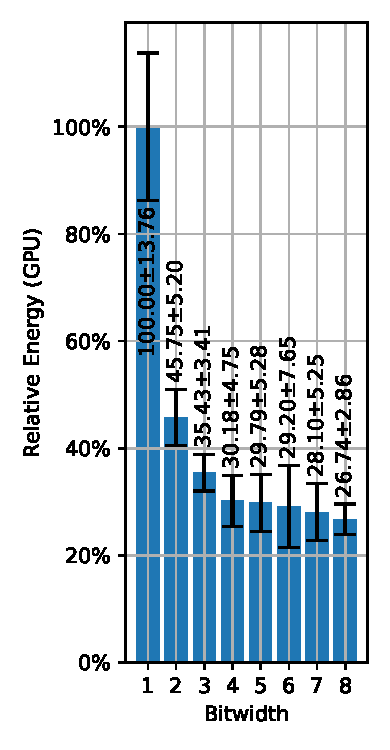
\includegraphics[width=\textwidth]{../standard/NMNIST/plots/nmnist_train_relative_energy_gpu.pdf}
                \caption{Normalized Energy Consumption Estimation Relative to 1-bit Spike Train Model}
            \end{subfigure}
            \caption{Training Energy Consumption Estimation on GPUs for NMNIST Dataset}
        \end{figure}

    \subsection{DVS Gesture}
    \label{appendix:energy_gpu_dvs_gesture}
        Launch command: Same as in Appendix \ref{appendix:accuracy_curves_dvs_gesture}

        \begin{figure}[H]
            \centering
            \begin{subfigure}[H]{0.48\textwidth}
                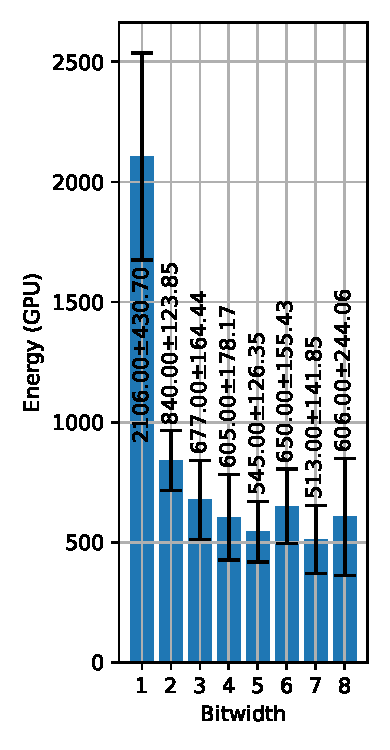
\includegraphics[width=\textwidth]{../standard/DVSGesture/plots/dvsgesture_train_energy_gpu.pdf}
                \caption{Energy Consumption Estimation, Unit in Constant $c$}
            \end{subfigure}
            \hfill
            \begin{subfigure}[H]{0.48\textwidth}
                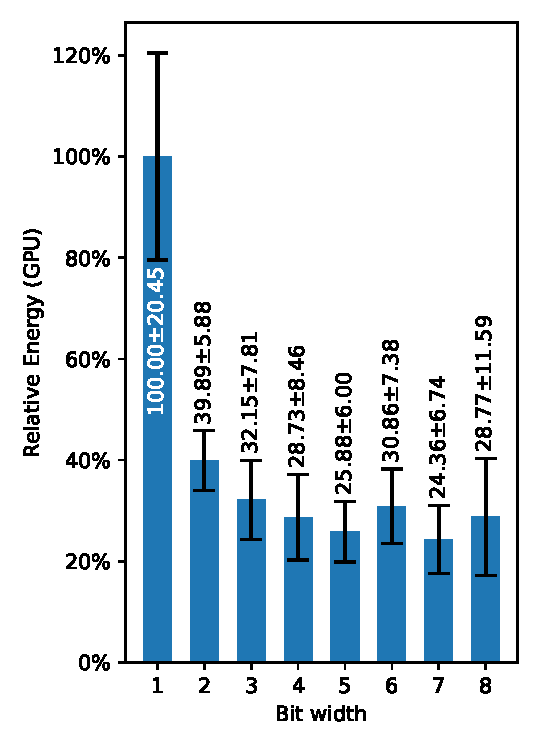
\includegraphics[width=\textwidth]{../standard/DVSGesture/plots/dvsgesture_train_relative_energy_gpu.pdf}
                \caption{Normalized Energy Consumption Estimation Relative to 1-bit Spike Train Model}
            \end{subfigure}
            \caption{Training Energy Consumption Estimation on GPUs for DVS Gesture Dataset}
        \end{figure}

    \subsection{CIFAR-10}
    \label{appendix:energy_gpu_cifar10}
        Launch command: Same as in Appendix \ref{appendix:accuracy_curves_cifar10}

        \begin{figure}[H]
            \centering
            \begin{subfigure}[H]{0.48\textwidth}
                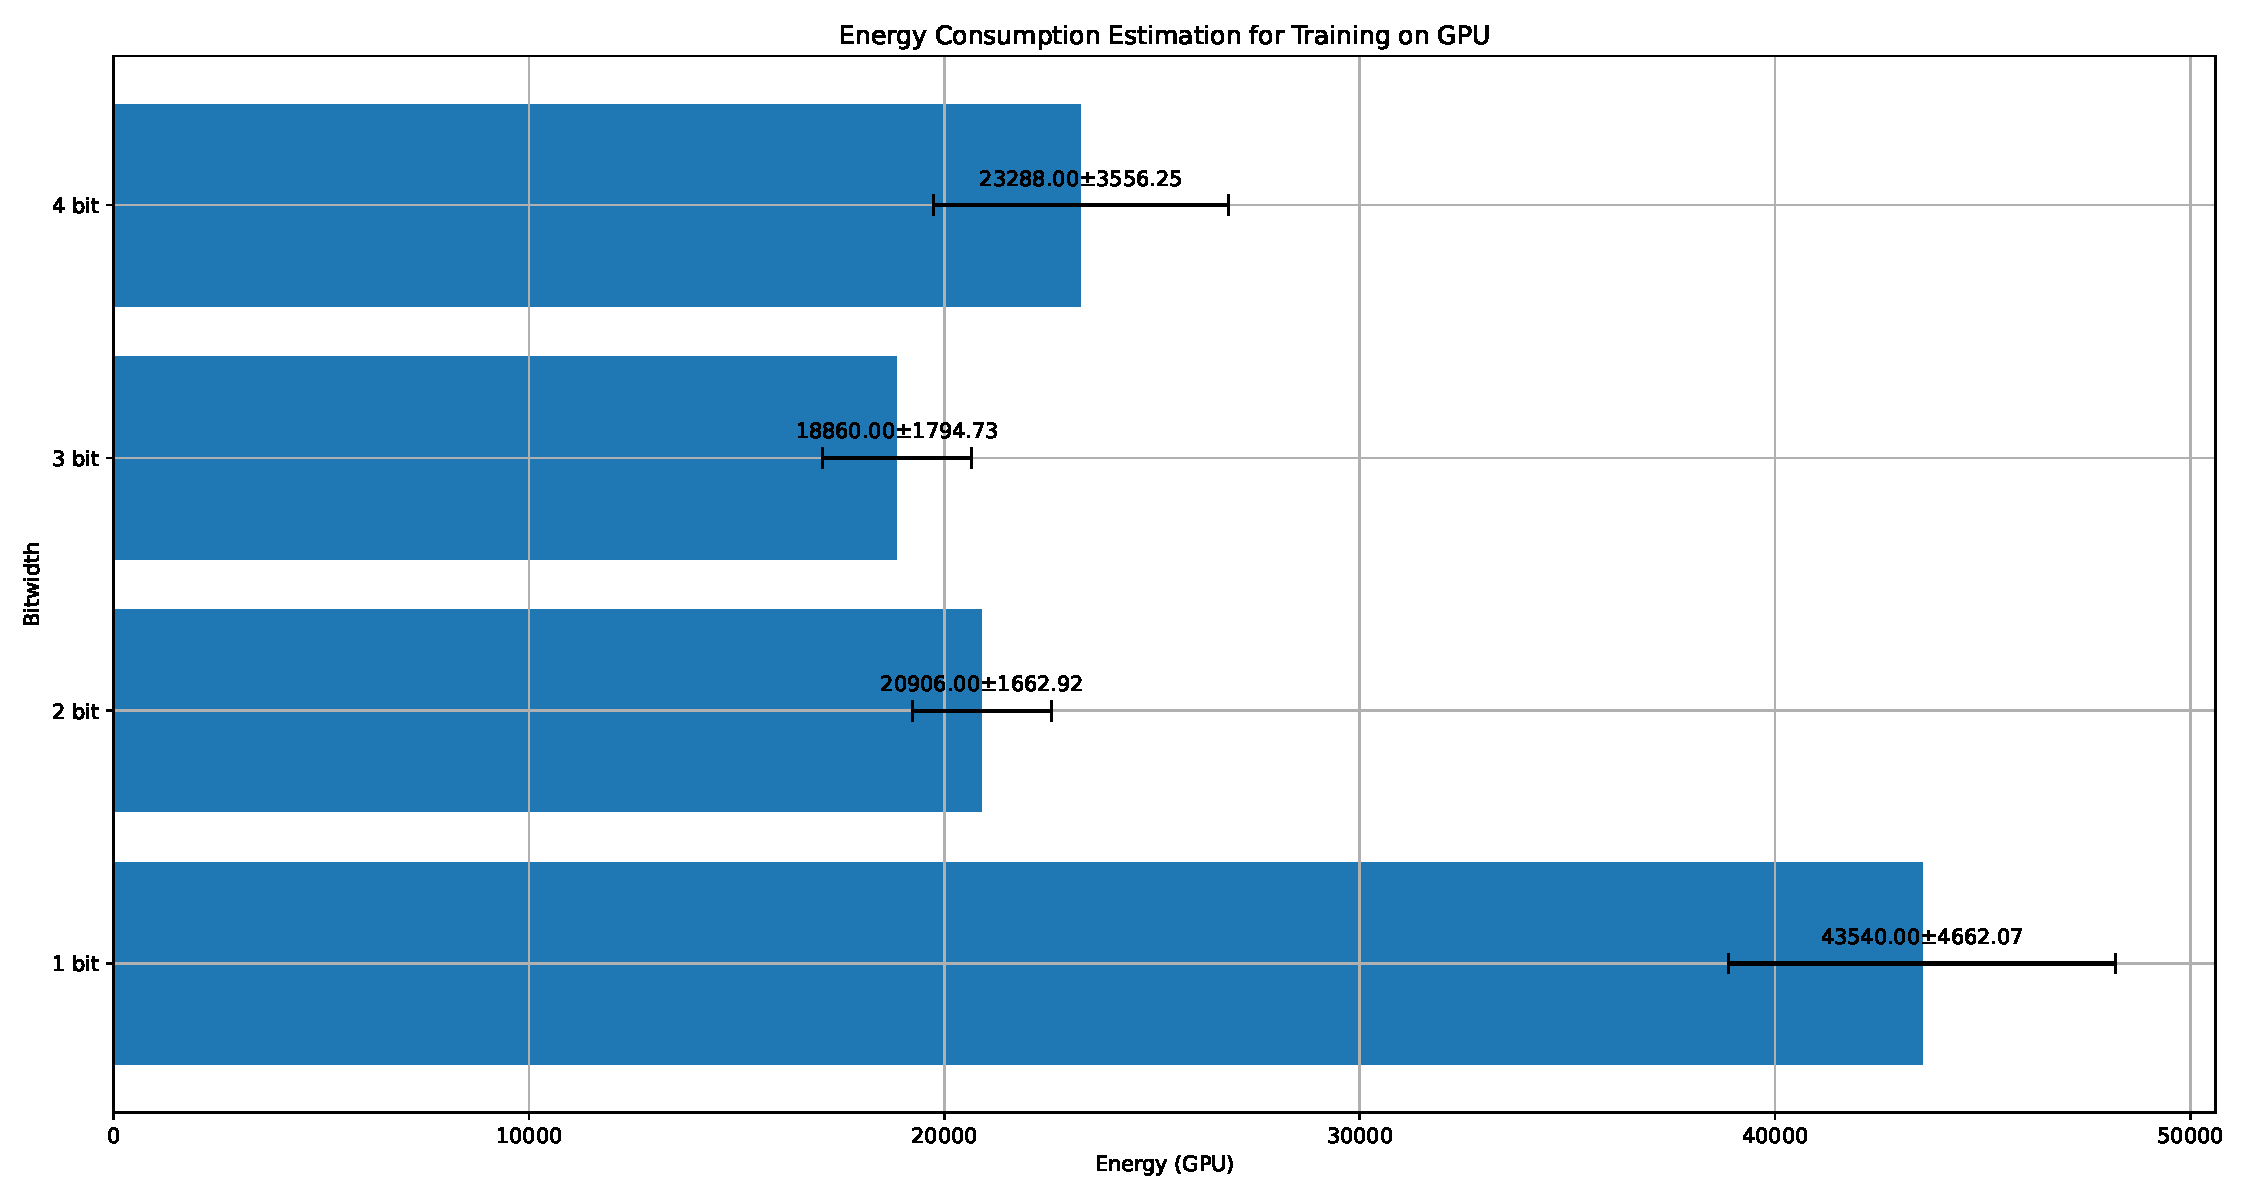
\includegraphics[width=\textwidth]{../standard/CIFAR10/plots/cifar10_train_energy_gpu.pdf}
                \caption{Energy Consumption Estimation, Unit in Constant $c$}
            \end{subfigure}
            \hfill
            \begin{subfigure}[H]{0.48\textwidth}
                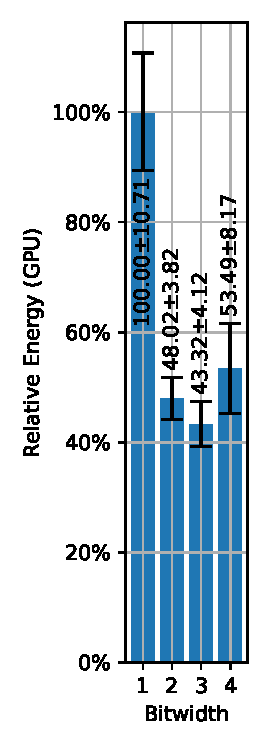
\includegraphics[width=\textwidth]{../standard/CIFAR10/plots/cifar10_train_relative_energy_gpu.pdf}
                \caption{Normalized Energy Consumption Estimation Relative to 1-bit Spike Train Model}
            \end{subfigure}
            \caption{Training Energy Consumption Estimation on GPUs for CIFAR-10 Dataset}
        \end{figure}

\section{Inference Energy Consumption Estimation on Neuromorphic Hardware}
\label{appendix:energy_neuromorphic}

    We assume the models are running on neuromorphic hardware like Intel Loihi 2 that support graded spikes. 

    \subsection{Fashion MNIST}
    \label{appendix:energy_neuromorphic_fashion_mnist}
        Launch command: Same as in Appendix \ref{appendix:accuracy_curves_fashion_mnist}

        \begin{figure}[H]
            \centering
            \begin{subfigure}[H]{0.495\textwidth}
                \includegraphics[width=\textwidth]{../standard/FashionMNIST/plots/fashionmnist_test_energy_nh.pdf}
                \caption{Energy Consumption Estimation, Unit in Parameters $F\cdot E_{\text{MAC}}$}
            \end{subfigure}
            \hfill
            \begin{subfigure}[H]{0.495\textwidth}
                \includegraphics[width=\textwidth]{../standard/FashionMNIST/plots/fashionmnist_test_relative_energy_nh.pdf}
                \caption{Normalized Energy Consumption Estimation Relative to 1-bit Spike Train Model}
            \end{subfigure}
            \caption{Inference Energy Consumption Estimation on Intel Loihi 2}
        \end{figure}
    
    \subsection{MNIST}
    \label{appendix:energy_neuromorphic_mnist}
        Launch command: Same as in Appendix \ref{appendix:accuracy_curves_mnist}

        \begin{figure}[H]
            \centering
            \begin{subfigure}[H]{\textwidth}
                \includegraphics[width=\textwidth]{../standard/MNIST/plots/mnist_test_energy_nh.pdf}
                \caption{Energy Consumption Estimation, Unit in Parameters $F\cdot E_{\text{MAC}}$}
            \end{subfigure}
            \hfill
            \begin{subfigure}[H]{\textwidth}
                \includegraphics[width=\textwidth]{../standard/MNIST/plots/mnist_test_relative_energy_nh.pdf}
                \caption{Normalized Energy Consumption Estimation Relative to 1-bit Spike Train Model}
            \end{subfigure}
            \caption{Inference Energy Consumption Estimation on Intel Loihi 2}
        \end{figure}

    \subsection{NMNIST}
    \label{appendix:energy_neuromorphic_nmnist}
        Launch command: Same as in Appendix \ref{appendix:accuracy_curves_nmnist}

        \begin{figure}[H]
            \centering
            \begin{subfigure}[H]{\textwidth}
                \includegraphics[width=\textwidth]{../standard/NMNIST/plots/nmnist_test_energy_nh.pdf}
                \caption{Energy Consumption Estimation, Unit in Parameters $F\cdot E_{\text{MAC}}$}
            \end{subfigure}
            \hfill
            \begin{subfigure}[H]{\textwidth}
                \includegraphics[width=\textwidth]{../standard/NMNIST/plots/nmnist_test_relative_energy_nh.pdf}
                \caption{Normalized Energy Consumption Estimation Relative to 1-bit Spike Train Model}
            \end{subfigure}
            \caption{Inference Energy Consumption Estimation on Intel Loihi 2}
        \end{figure}

    \subsection{DVS Gesture}
    \label{appendix:energy_neuromorphic_dvs_gesture}
        Launch command: Same as in Appendix \ref{appendix:accuracy_curves_dvs_gesture}

        \begin{figure}[H]
            \centering
            \begin{subfigure}[H]{\textwidth}
                \includegraphics[width=\textwidth]{../standard/DVSGesture/plots/dvsgesture_test_energy_nh.pdf}
                \caption{Energy Consumption Estimation, Unit in Parameters $F\cdot E_{\text{MAC}}$}
            \end{subfigure}
            \hfill
            \begin{subfigure}[H]{\textwidth}
                \includegraphics[width=\textwidth]{../standard/DVSGesture/plots/dvsgesture_test_relative_energy_nh.pdf}
                \caption{Normalized Energy Consumption Estimation Relative to 1-bit Spike Train Model}
            \end{subfigure}
            \caption{Inference Energy Consumption Estimation on Intel Loihi 2}
        \end{figure}

    \subsection{CIFAR-10}
    \label{appendix:energy_neuromorphic_cifar10}
        Launch command: Same as in Appendix \ref{appendix:accuracy_curves_cifar10}

        \begin{figure}[H]
            \centering
            \begin{subfigure}[H]{\textwidth}
                \includegraphics[width=\textwidth]{../standard/CIFAR10/plots/cifar10_test_energy_nh.pdf}
                \caption{Energy Consumption Estimation, Unit in Parameters $F\cdot E_{\text{MAC}}$}
            \end{subfigure}
            \hfill
            \begin{subfigure}[H]{\textwidth}
                \includegraphics[width=\textwidth]{../standard/CIFAR10/plots/cifar10_test_relative_energy_nh.pdf}
                \caption{Normalized Energy Consumption Estimation Relative to 1-bit Spike Train Model}
            \end{subfigure}
            \caption{Inference Energy Consumption Estimation on Intel Loihi 2}
        \end{figure}

\section{Trading Accuracy for Energy Consumption}
\label{appendix:energy_tradeoff}

    \subsection{Fashion MNIST}
    \label{appendix:energy_tradeoff_fashion_mnist}
        Launch command: 
        \begin{lstlisting}[language=Bash, basicstyle=\small, breaklines=true]
python -m test --N 2 --R 10 --T 10 4 --acc 0.80 --model FashionMNISTNet --data-path /scratch/zyi/codeSpace/data --dataset FashionMNIST --batch-size 128 --opt adam --lr 2e-3 --lr-scheduler none --epochs 5 --lr-warmup-epochs 0 --output-dir /scratch/zyi/codeSpace/MultibitSpikes/timesteps --mixup-alpha 0.0 --cutmix-alpha 0.0 --label-smoothing 0.0 --disable-amp
        \end{lstlisting}

        \begin{figure}[H]
            \centering
            \begin{subfigure}[H]{0.48\textwidth}
                \includegraphics[width=\textwidth]{../timesteps/FashionMNIST/plots/fashionmnist_train_acc.pdf}
                \caption{Training Accuracy (smoothed with a window size of 100)}
            \end{subfigure}
            \hfill
            \begin{subfigure}[H]{0.48\textwidth}
                \includegraphics[width=\textwidth]{../timesteps/FashionMNIST/plots/fashionmnist_test_acc.pdf}
                \caption{Test Accuracy}
            \end{subfigure}
            \hfill
            \begin{subfigure}[H]{\textwidth}
                \includegraphics[width=\textwidth]{../timesteps/FashionMNIST/plots/fashionmnist_final_acc.pdf}
                \caption{Final Test Accuracy}
            \end{subfigure}
            \caption{Accuracy of 1-bit Spike Train Model with 10 Timesteps and 2-bit Spike Train Model with 4 Timesteps}
        \end{figure}

        \begin{figure}[H]
            \centering
            \begin{subfigure}[H]{0.48\textwidth}
                \includegraphics[width=\textwidth]{../timesteps/FashionMNIST/plots/fashionmnist_train_energy_gpu.pdf}
                \caption{Energy Consumption Estimation, Unit in Constant $c$}
            \end{subfigure}
            \hfill
            \begin{subfigure}[H]{0.48\textwidth}
                \includegraphics[width=\textwidth]{../timesteps/FashionMNIST/plots/fashionmnist_train_relative_energy_gpu.pdf}
                \caption{Normalized Energy Consumption Estimation Relative to 1-bit Spike Train Model}
            \end{subfigure}
            \caption{Training Energy Consumption Estimation on GPUs for Fashion MNIST Dataset}
        \end{figure}

        \begin{figure}[H]
            \centering
            \begin{subfigure}[H]{0.48\textwidth}
                \includegraphics[width=\textwidth]{../timesteps/FashionMNIST/plots/fashionmnist_test_energy_nh.pdf}
                \caption{Energy Consumption Estimation, Unit in Parameters $F\cdot E_{\text{MAC}}$}
            \end{subfigure}
            \hfill
            \begin{subfigure}[H]{0.48\textwidth}
                \includegraphics[width=\textwidth]{../timesteps/FashionMNIST/plots/fashionmnist_test_relative_energy_nh.pdf}
                \caption{Normalized Energy Consumption Estimation Relative to 1-bit Spike Train Model}
            \end{subfigure}
            \caption{Inference Energy Consumption Estimation on Intel Loihi 2}
        \end{figure}

    \subsection{CIFAR-10}
    \label{appendix:energy_tradeoff_cifar10}
        Launch command: 
        \begin{lstlisting}[language=Bash, basicstyle=\small, breaklines=true]
python -m test --N 2 --R 5 --T 10 4 --acc 0.80 --model CIFAR10Net --data-path /scratch/zyi/codeSpace/data --dataset CIFAR10 --batch-size 128 --opt adam --lr 1e-5 --lr-scheduler none --epochs 50 --lr-warmup-epochs 0 --output-dir /scratch/zyi/codeSpace/MultibitSpikes/timesteps
        \end{lstlisting}

        \begin{figure}[H]
            \centering
            \begin{subfigure}[H]{0.48\textwidth}
                \includegraphics[width=\textwidth]{../timesteps/CIFAR10/plots/cifar10_train_acc.pdf}
                \caption{Training Accuracy (smoothed with a window size of 100)}
            \end{subfigure}
            \hfill
            \begin{subfigure}[H]{0.48\textwidth}
                \includegraphics[width=\textwidth]{../timesteps/CIFAR10/plots/cifar10_test_acc.pdf}
                \caption{Test Accuracy}
            \end{subfigure}
            \hfill
            \begin{subfigure}[H]{\textwidth}
                \includegraphics[width=\textwidth]{../timesteps/CIFAR10/plots/cifar10_final_acc.pdf}
                \caption{Final Test Accuracy}
            \end{subfigure}
            \caption{Accuracy of 1-bit Spike Train Model with 10 Timesteps and 2-bit Spike Train Model with 4 Timesteps}
        \end{figure}

        \begin{figure}[H]
            \centering
            \begin{subfigure}[H]{0.48\textwidth}
                \includegraphics[width=\textwidth]{../timesteps/CIFAR10/plots/cifar10_train_energy_gpu.pdf}
                \caption{Energy Consumption Estimation, Unit in Constant $c$}
            \end{subfigure}
            \hfill
            \begin{subfigure}[H]{0.48\textwidth}
                \includegraphics[width=\textwidth]{../timesteps/CIFAR10/plots/cifar10_train_relative_energy_gpu.pdf}
                \caption{Normalized Energy Consumption Estimation Relative to 1-bit Spike Train Model}
            \end{subfigure}
            \caption{Training Energy Consumption Estimation on GPUs for CIFAR-10 Dataset}
        \end{figure}

        \begin{figure}[H]
            \centering
            \begin{subfigure}[H]{0.48\textwidth}
                \includegraphics[width=\textwidth]{../timesteps/CIFAR10/plots/cifar10_test_energy_nh.pdf}
                \caption{Energy Consumption Estimation, Unit in Parameters $F\cdot E_{\text{MAC}}$}
            \end{subfigure}
            \hfill
            \begin{subfigure}[H]{0.48\textwidth}
                \includegraphics[width=\textwidth]{../timesteps/CIFAR10/plots/cifar10_test_relative_energy_nh.pdf}
                \caption{Normalized Energy Consumption Estimation Relative to 1-bit Spike Train Model}
            \end{subfigure}
            \caption{Inference Energy Consumption Estimation on Intel Loihi 2}
        \end{figure}
